\chapter{Introduction}\label{sec:introduction}

%SOME MORE GENERAL INTRO TEXT HERE?
The ability to understand spoken language, to recognize faces and to distinguish types of fruit comes naturally to humans, even though these processes of pattern recognition and classification are inherently complex. Machine learning (ML), a subtopic of artificial intelligence, is concerned with the development of algorithms that perform these types of tasks, thus enabling computers to find and recognise patterns in data and classify unknown inputs based on previous training with labelled inputs. Such algorithms make the core of e.g. human speech recognition and recommendation engines as used by Amazon.
% and algorithms that can predict heart disease from real-time electrocardiograms \citep{acharya2015integrated, pazzani2007content}.

According to \citeA{bigdata}, approximately 2.5 quintillion (${10}^{18}$) bytes of digital data are created every day. This growing number implies that every area dealing with data will eventually require advanced algorithms that can make sense of data content, retrieve patterns and reveal correlations. However, most ML algorithms involve the execution of computationally expensive operations and doing so on large data sets inevitably takes a lot of time \cite{bekkerman2011scaling}. Thus, it becomes increasingly important to find efficient ways of dealing with big data.
%and/or reduce the computational complexity of the algorithms.

A promising solution is the use of quantum computation which has been researched intensively in the last few decades. Quantum computers (QCs) use quantum mechanical systems and their special properties to manipulate and process information in ways that are impossible to implement on classical computers. The quantum equivalent to a classical bit is called a quantum bit (qubit) and additionally to being in either state \0 or \1 it can be in their linear superposition.

%\begin{equation}
%\label{equ: simplequbit}
%\ket{q} = \alpha \ket{0} + \beta \ket{1}
%\end{equation}
%where $\alpha$ and $\beta$ are complex numbers and often referred to as amplitudes. When measuring qubit $\ket{q}$ it will take the value \0 with a probability of ${|\alpha|}^{2}$ and \1 with a probability of ${|\beta|}^{2}$. Since the total probability has to sum to unity, the normalization condition ${|\alpha|}^{2} + {|\beta|}^{2} =  1$ must be satisfied at all times.

This peculiar property gives rise to so-called quantum parallelism, which enables the execution of certain operations on many quantum states at the same time. Despite this advantage, the difficulty in quantum computation lies in the retrieval of the computed solution since a measurement of a qubit collapses it into a single classical bit and thereby destroys information about its previous superposition. Several quantum algorithms have been proposed that provide exponential speed-ups when compared to their classical counterparts with Shor's prime factorization algorithm being the most famous \cite{shor1994}.
%As another example, Grover's quantum database search algorithm enables finding a single element in a list of $N$ elements within roughly $\sqrt{N}$ quantum mechanical steps instead of $N$ classical steps \citep{grover}.
Hence, quantum computation has the potential to vastly improve computational power, speed up the processing of big data and solve certain problems that are practically unsolvable on classical computers. 

%for the QML toolbox to be complete a quantum algorithm to solve systems of linear equations is needed since most ML algorithms rely on solving those.

Considering these advantages, the combination of quantum computation and classical ML into the new field of quantum machine learning (QML) seems almost natural. There are currently two main ideas on how to merge quantum computation with ML, namely a) running the classical algorithm on a classical computer and outsourcing only the computationally intensive task to a QC or b) executing the quantum version of the entire algorithm on a QC. Current QML research mostly focusses on the latter approach by developing quantum algorithms that tap into the full potential of quantum parallelism.

\section{Motivation}
\label{sec:motivation}

Classical ML is a very practical topic since it can be directly tested, verified and implemented on any commercial classical computer. So far, QML has been of almost entirely theoretical nature since the required computational resources are not in place yet. To yield reliable solutions QML algorithms often require a relatively large number of error-corrected qubits and some sort of quantum data storage such as the proposed quantum random access memory (qRAM) \cite{qRAM}. However, to date the maximum number of superconducting qubits reportedly used for calculation is nine, the D-Wave II quantum annealing device delivers 1152 qubits but can only solve a narrow class of problems and a qRAM has not been developed yet \cite{hydrogensimulation, dwave2}. Furthermore, qubit error-correction is still a very active research field and most of the described preliminary QCs deal with non error-corrected qubits with short lifetimes and are, thus, impractical for large QML implementations.

Until now there have been only few experimental verifications of QML algorithms that establish proof-of-concept. \citeA{Li2015} successfully distinguished a handwritten six from a nine using a quantum support vector machine on a four-qubit nuclear magnetic resonance test bench. In addition, \citeA{Cai2015} were first to experimentally demonstrate quantum machine learning on a photonic QC and showed that the distance between two vectors and their inner product can indeed be computed quantum mechanically. Lastly, \citeA{Riste2015} solved a learning parity problem with five superconducting qubits and found that a quantum advantage can already be observed in non error-corrected systems.

%Consequently,
Considering the gap between the number of proposed QML algorithms and the few experimental realisations, it remains important to find QML problems which can already be implemented on small-scale QCs. Hence, the purpose of this study is to provide proof-of-concept implementation of selected QML algorithms on small datasets. This is an important step in the attempt to shift QML from a purely theoretical research area to a more applied field such as classical ML. 

\section{Research question}
\label{sec:researchquestion}


%Don't know where this should go!

%Matthias Troyer citation for this part:

%There are many different ways of realising a QC such as using trapped ions, single photon sources or superconducting Josephson junctions, etc. Depending on the chosen substrate, different sets of quantum logic gates can be implemented and in order to run a quantum algorithm  it has to be mapped to the available hardware. Thus, quantum algorithms have to be translated (compiled) into a series of gates consisting only of quantum gates from the available gate set. This is referred to as \emph{quantum compilation}.

%Finding optimal ways of compiling a given quantum algorithm as well as designing a high-level programming language or environment similar to that of classical computer code editors is called \emph{quantum software engineering}.

In light of the theoretical nature of current QML research and the small number of experimental realizations, this research will address the following question:

%NARROW DOWN THE RESEARCH QUESTION!
\centering\textbf{How can a k-nearest neighbour quantum machine learning algorithm be implemented on small-scale quantum computers?}

%Alternatives:
%Is it possible to experimentally demonstrate that two QML algorithms proposed by \cite{Schuld2014, Schuld2016} can already solve a small ML problem using classical simulation or IBMs quantum processor?
%Is it possible to already implement and solve a small ML problem on IBMs publicly available quantum computer?

\justify
The following sections will outline the steps required and the tools used in order to answer this research question. 

\chapter{Theoretical Foundations}\label{sec:theory}
\section{Quantum bits}
\label{subsec:qubits}
\subsection{Single qubit systems}
\label{subsubsec:qubits}
%Classical computers manipulate bits and the quantum equivalent is called a quantum bit, often abbreviated as qubit.
Classical computers manipulate bits, whereas quantum computer's most fundamental unit is called a quantum bit, often abbreviated as qubit. Bits as well as qubits are binary entities, meaning they can only take the values 0 and 1.

A good example for a physical implementation of a qubit is the single electron of a hydrogen atom sketched in Fig.~\ref{img:qubitatom}. Usually, the electron is found in its ground state which one can define as the \0 state of the qubit. Using a laser pulse the electron can be excited into the next highest valence shell which one can define as the \1 state of the qubit. After some time $t$ the electron will decohere to its ground state (\0) which is called the longitudinal coherence or amplitude damping time and is an important parameter for measuring qubit lifetimes.

\begin{figure}[!ht]
       \centering
       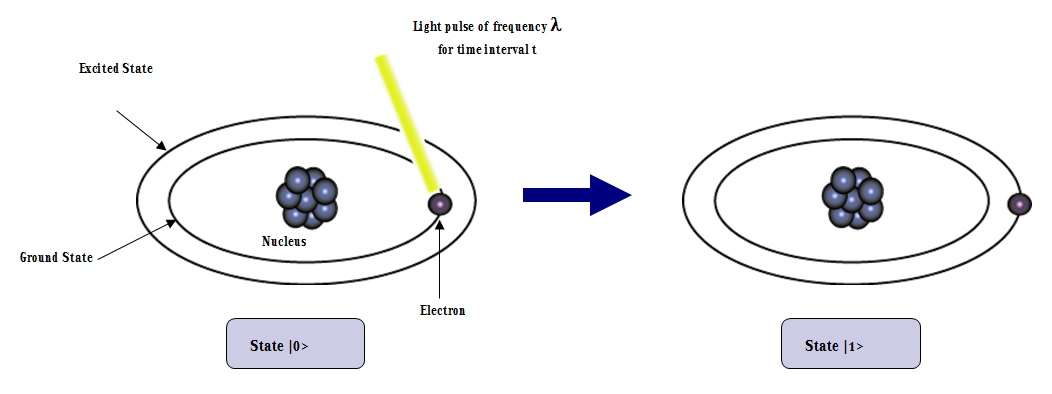
\includegraphics[scale=0.35]{img/qubitimplementation.jpeg}
       \caption[]{\label{img:qubitatom} A simple example of a physical qubit using the electron of a hydrogen atom\textsuperscript{1}}
\end{figure}

\footnotetext[1]{Reprinted from RF Wireless World, n.d., Retrieved December 23, 2016, from \url{http://www.rfwireless-world.com/Terminology/Difference-between-Bit-and-Qubit.html}. Copyright 2012 by RF Wireless World. Reprinted with permission.}
\pagebreak
A classical non-probabilistic bit can only be in one of the two possible states at once. In contrast, qubits obey the laws of quantum mechanics, which gives rise to the powerful property that - besides being a definite 0 or 1 - they can also be in a superposition of the two states. Mathematically this is expressed as a linear combination of the states 0 and 1:

\begin{equation}
\label{equ: simplequbit}
\ket{\psi} = \alpha \ket{0} + \beta \ket{1}
\end{equation}

where $\alpha$ and $\beta$ are complex coefficients ($\alpha, \beta \in \mathbb{C}$) and are often referred to as amplitudes. Any amplitude $\eta$ can be further subdivided into a complex phase factor $e^{i\phi}$ and a non-negative real number $e$ such that,


\begin{equation}
\label{equ: amplitude}
\eta = e^{i\phi}e
\end{equation}

In Equ.~\ref{equ: simplequbit}, \0 is the Dirac notation for the qubit being in state 0 and it represents a two-dimensional vector in a complex 2-D vector space (called Hilbert space $\mathcal{H}_{2}$). \0 and \1 are the computational basis states and they constitute an orthonormal basis of $\mathcal{H}_{2}$. For the sake of clarity, \0 and \1 can be thought of as the 2-D vectors shown below.

APPROXIMATELY EQUAL SIGN!
\begin{equation}
\label{equ: 0and1kets}
\ket{0} =  \colvec{1\\0} \quad \quad \ket{1} = \colvec{0\\1}
\end{equation}

Subbing these vectors into Equ.~\ref{equ: simplequbit} yields the vector representation of $\ket{\psi}$:
\begin{equation}
\label{equ: simplequbitvector}
\ket{\psi} = \alpha \colvec{1\\0} + \beta \colvec{0\\1} = \colvec{\alpha\\\beta}
\end{equation}

In the cases $\alpha = 1$ or $\beta = 1$ there is no quantum behaviour since the qubit is not in a superposition. However, if for example $\alpha = \beta = \frac{1}{\sqrt{2}}$ the qubit is in an equal quantum superposition which is impossible to achieve with a classical computer. This leads to another important qubit lifetime parameter - the transversal coherence or phase damping time. It is measured by preparing the equal superposition $\frac{\ket{0}+\ket{1}}{\sqrt{2}}$ and due to unavoidable interaction with the environment after some time $t$ the quantum behaviour will be lost and the state will either be a definite \0 or \1. The process of losing quantum behaviour is called \emph{decoherence}.

However, even though a qubit can be in a superposition of \0 and \1, when measured it will take the value \0 with a probability of
\begin{equation}
\label{equ:bornrule0}
Prob(\ket{0}) = {|\alpha|}^{2}
\end{equation}
and \1 with a probability of 
\begin{equation}
\label{equ:bornrule1}
Prob(\ket{1}) = {|\beta|}^{2}
\end{equation}

The fact that the probability of measuring a particular state is equal the absolute value squared of the respective amplitude is called Born rule (citation). Since the total probability of measuring any value has to be 1, the following normalization condition must be satisfied:
\begin{equation}
\label{equ: normalization}
{|\alpha|}^{2} + {|\beta|}^{2} =  1
\end{equation}

\newpage
Therefore, a qubit is inherently probabilistic but when measured it collapses into a single classical bit (0 or 1). It follows that a measurement destroys information about the superposition of the qubit (the values of $\alpha$ and $\beta$). This constitutes one of the main difficulties when designing quantum algorithms since only limited information can be obtained about the final states of the qubits in the quantum computer.

Using spherical polar coordinates, a single qubit can be visualized on the so-called Bloch sphere by parameterising $\alpha$ and $\beta$ in Equ.~\ref{equ: simplequbit} as follows:

\begin{equation}
\label{equ: blochqubit}
\ket{q} = \cos\frac{\theta}{2} \ket{0} + e^{i \phi} \sin\frac{\theta}{2} \ket{1}
\end{equation}

The Bloch sphere has a radius of 1 and is therefore a unit sphere. The \0 qubit state is defined to lie along the positive z-axis ($\hat{z}$) and the \1 state is defined to lie along the negative z-axis ($-\hat{z}$) as labelled in Fig.~\ref{fig:blochsphere}. At this point, it is important to note that these two states are mutually orthogonal in $\mathcal{H}_{2}$ even though they are not orthogonal on the Bloch sphere. 

Qubit states on the Bloch equator such as the $\hat{x}$ and $\hat{y}$ coordinate axes represent equal superpositions where \0 and \1 both have measurement probabilities equal to $0.5$. The $\hat{x}$-axis for example represents the equal superposition $\ket{q} = \frac{1}{\sqrt{2}} \ket{0} + \frac{1}{\sqrt{2}} \ket{1}$. As illustrated in Fig.~\ref{fig:blochsphere} any arbitrary 2-D qubit state $\ket{\psi}$ can be decomposed into the polar angles $\theta$ and $\phi$ and visualized as a vector on the Bloch sphere. Such an object is called the Bloch vector of the qubit state $\ket{\psi}$. The Bloch sphere will be the main visualization tool for qubit manipulations in this thesis.

\begin{figure}[!ht]
       \centering
       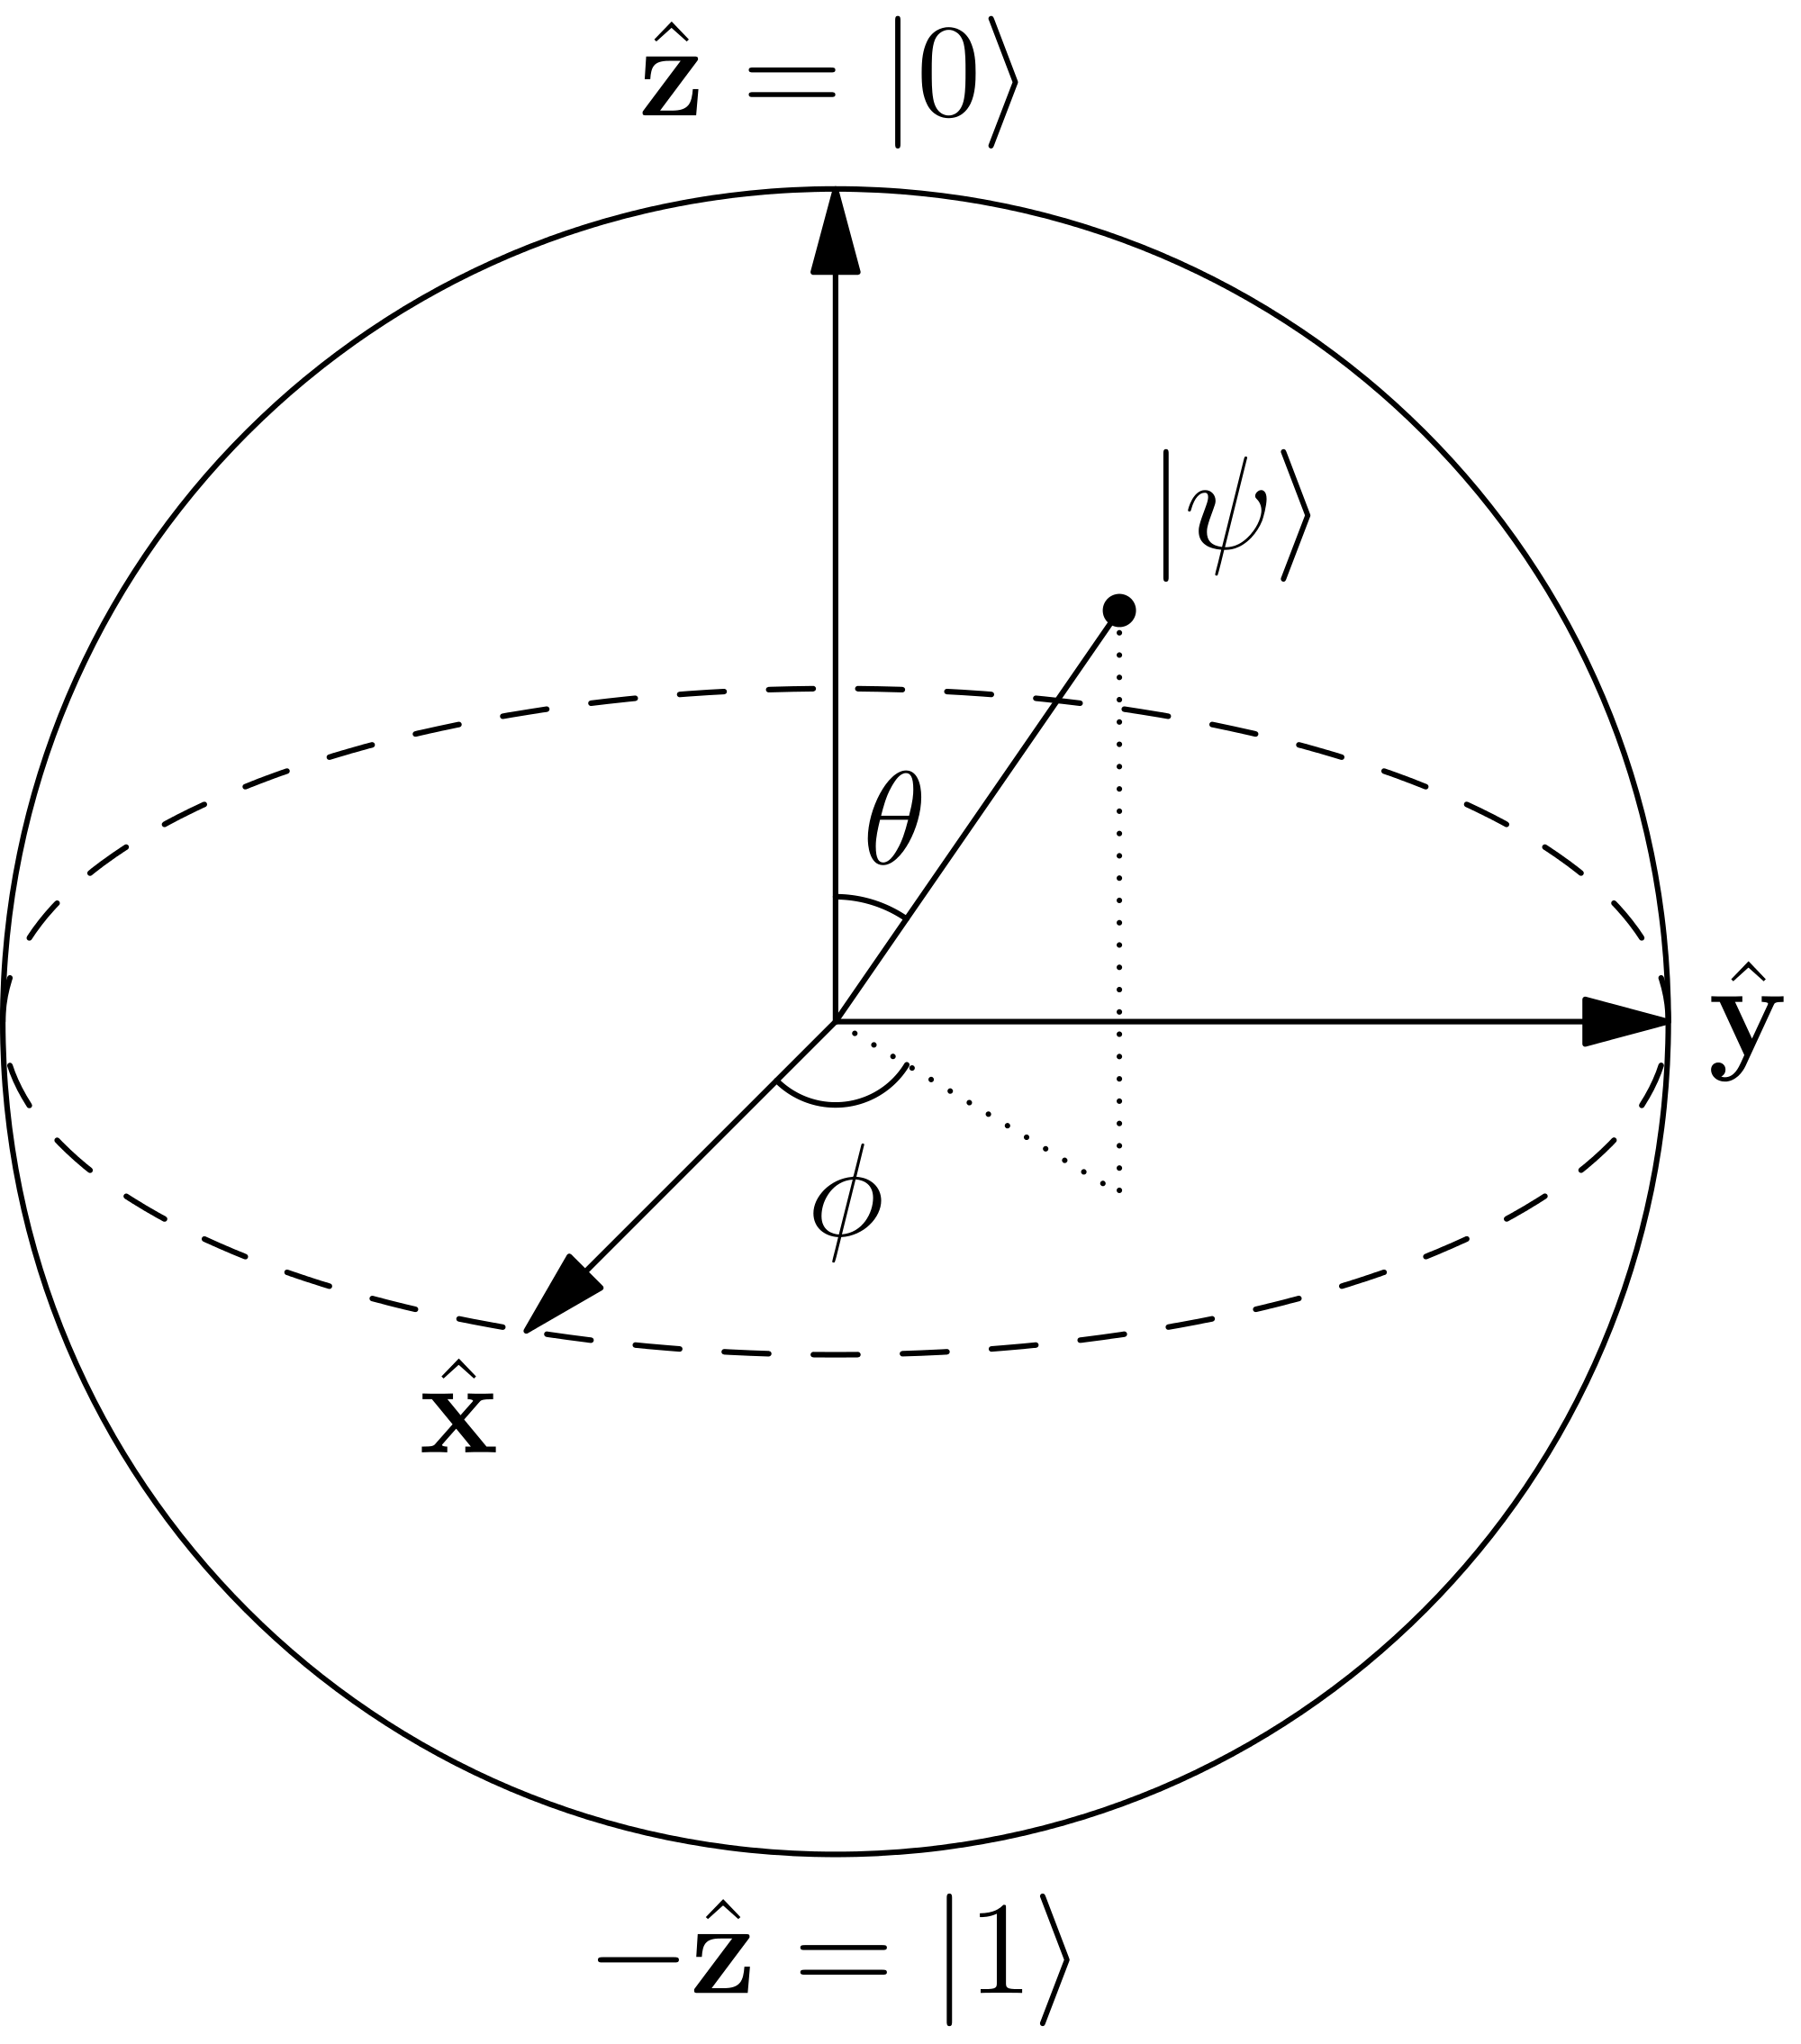
\includegraphics[scale=0.07]{img/blochsphere.png}
       \caption[]{\label{fig:blochsphere} An arbitrary two-dimensional qubit $\ket{\psi}$ visualized on the Bloch sphere.\footnotemark[2]}
\end{figure}

\footnotetext[2]{Reprinted from Wikipedia, n.d., Retrieved September 7, 2016, from \url{https://en.wikipedia.org/wiki/Bloch_Sphere}. Copyright 2012 by Glosser.ca. Reprinted with permission.}


Similar to logic gates in a classical computer, a QC manipulates qubit by means of quantum logic gates which will be introduced in detail in Section~\ref{subsec:quantumlogicgates}. Generally, an arbitrary quantum logic gate U acting on a single qubit state is a linear transformation given by a 2x2 matrix whose action on $\ket{\psi}$ is defined as:

\begin{equation}
\label{equ:unitarytransformation}
U \ket{\psi} = \begin{pmatrix}
 a & b \\ 
 c & d
 \end{pmatrix} \colvec{\alpha\\\beta} = \colvec{a*\alpha+b*\beta\\c*\alpha+d*\beta}
\end{equation}

Matrix $U$ must be unitary which means that a) its determinant is equal to unity and b) its Hermitian conjugate $U^\dagger$ must be equal to its inverse (see Equ.~\ref{equ:unitarydef1} and ~\ref{equ:unitarydef2}). All quantum logic gates must be unitary since this preserves the normalization of the qubit state it is acting on.

\begin{align}
\label{equ:unitarydef1}
a)& \mid det(U) \mid = 1 \\ 
\label{equ:unitarydef2}
b)& \quad UU^\dagger = U^\dagger U = \mathbb{1} = UU^{-1} = U^{-1}U
\end{align} 

The set of all 2-D complex unitary matrices with determinant one is called the special unitary group $SU(2)$ and all single-qubit quantum gates are therefore elements of $SU(2)$. Furthermore, a gate set $G$ consisting of $m$ quantum-gates $g_1,g_2,...,g_m$ is called a \emph{universal quantum gate set} when it is a dense subset of $SU(2)$ as defined in the red box below.

\begin{redbox}
\textbf{Definition: Dense Subset of $SU(2)$}\\
\newline
The gate set $G$ is a dense subset of $SU(2)$ when given any quantum gate $W \in SU(2)$ and any accuracy $\epsilon > 0$ there exists a product $J$ of gates from $G$ which is an $\epsilon$-approximation to $W$ \cite{dawson2005solovay}.
\end{redbox}

\subsection{Multi qubit systems}
\label{subsec:multiqubitsystems}

A classical computer with one bit of memory is not particularly useful and equally a QC with one qubit is rather useless. In order to be able to perform large and complicated computations many individual qubits need to be combined to create a large QC. When moving from single to multi qubit systems a new mathematical tool, the so-called tensor product (symbol $\otimes$), is needed. A tensor product of two qubits is written as:

\begin{equation}
\ket{\psi} \otimes \ket{\psi} = \ket{0} \otimes \ket{0} = \ket{00}
\end{equation}
 
whereby the last expression omits the $\otimes$ symbol which is the shorthand form of a tensor product between two qubits. A \emph{quantum register} of size $j$ is an alternative way of referring to a tensor product of $j$ qubits. In QML algorithms, large quantum states are usually subdivided into several quantum registers fulfilling different purposes e.g. storing data or class label.

In vector notation a tensor product of two vectors (\textcolor{red}{red} and \textcolor{green}{green}) is defined as shown below:

\begin{equation}
\label{equ:tensor2qubits}
\ket{\textcolor{red}{0}\textcolor{green}{0}} = \textcolor{red}{\ket{0}} \otimes \textcolor{green}{\ket{0}} = \textcolor{red}{\colvec{1\\0}} \otimes \textcolor{green}{\colvec{1\\0}} = \colvec{\textcolor{red}{1}*\textcolor{green}{\colvec{1\\0}}\\\textcolor{red}{0}*\textcolor{green}{\colvec{1\\0}}} = \colvec{1\\0\\0\\0}
\end{equation}

The last expression in Equ.~\ref{equ:tensor2qubits} shows that the two-qubit state $\ket{00}$ is no longer two but four-dimensional. Hence, it lives in a four-dimensional Hilbert space $\mathcal{H}_{4}$. A quantum gate acting on multiple qubits can therefore not have the same dimensions as a single-qubit gate (Equ.~\ref{equ:unitarytransformation}) which demands for a new gate formalism for multi qubit systems.

Consider wanting to apply an arbitrary single-qubit gate U (Equ.~\ref{equ:unitarytransformation}) to the first qubit and leaving the second qubit unchanged, essentially applying the identity matrix $\mathbb{1}$ to it. To do this, one defines the tensor product of two matrices as follows,

\begin{equation}
\label{equ:matrixtensorproduct}
\textcolor{red}{U} \otimes \textcolor{green}{\mathbb{1}} =\textcolor{red}{\begin{pmatrix}
 a & b \\ 
 c & d
 \end{pmatrix}} \otimes \textcolor{green}{\begin{pmatrix}
 1 & 0 \\ 
 0 & 1
 \end{pmatrix}} = \begin{pmatrix}
 \textcolor{red}{a}*\textcolor{green}{\begin{pmatrix}
 1 & 0 \\ 
 0 & 1
 \end{pmatrix}} & \textcolor{red}{b}*\textcolor{green}{\begin{pmatrix}
 1 & 0 \\ 
 0 & 1
 \end{pmatrix}} \\ 
 \textcolor{red}{c}*\textcolor{green}{\begin{pmatrix}
 1 & 0 \\ 
 0 & 1
 \end{pmatrix}} & \textcolor{red}{d}*\textcolor{green}{\begin{pmatrix}
 1 & 0 \\ 
 0 & 1
 \end{pmatrix}}
 \end{pmatrix} = \begin{pmatrix}
 a & 0 & b & 0 \\ 
 0 & a & 0 & b \\ 
 c & 0 & d & 0 \\ 
 0 & c & 0 & d 
 \end{pmatrix}
\end{equation}

Thus, the result of the tensor product $U \otimes \mathbb{1}$ is a unitary 4x4 matrix which can now be used to linearly transform the 4x1 vector representing the $\ket{00}$ state in Equ.~\ref{equ:tensor2qubits}:

\begin{equation}
\label{equ:2qubitlineartransform1}
U \otimes \mathbb{1} \ket{00} = \begin{pmatrix}
 a & 0 & b & 0 \\ 
 0 & a & 0 & b \\ 
 c & 0 & d & 0 \\ 
 0 & c & 0 & d 
 \end{pmatrix} \colvec{1\\0\\0\\0} = \colvec{a\\0\\c\\0}
\end{equation}

One can also first perform the single qubit operations on the respective qubits followed by the tensor product of the two resulting vectors:

\begin{equation}
\label{equ:2qubitlineartransform2}
(U \otimes \mathbb{1})(\ket{0} \otimes \ket{0})= U\ket{0} \otimes \mathbb{1}\ket{0} = \begin{pmatrix}
 a & b \\ 
 c & d
 \end{pmatrix} \colvec{1\\0} \otimes \begin{pmatrix}
 1 & 0 \\ 
 0 & 1
 \end{pmatrix} \colvec{1\\0} = \colvec{a\\c} \otimes \colvec{1\\0} = \colvec{a\\0\\c\\0}
\end{equation}

This formalism can be extended to any number of qubits and the use of tensor products leads to an exponential increase in the dimensionality of the Hilbert space. Hence, $n$ qubits live in a $2^n$-dimensional Hilbert space ($\mathcal{H}_{2}^{\otimes n}$) and can store the content of $2^n$ classical bits. As an example, only 33 qubits can store the equivalent of $2^{33} = 8,589,934,592$ bits (= 1 gigabyte) which clearly bears the potential for enourmous speed-ups in computations as will be demonstrated later.

When considering multi qubit systems one will encounter quantum states that can or cannot be factorized. Consider for example the last expression in Equ.~\ref{equ:2qubitlineartransform2} which can be reexpressed as follows,

\begin{equation}
\label{equ:2qubitreexpressed}
\colvec{a\\0\\c\\0} = a\colvec{1\\0\\0\\0} + 0\colvec{0\\1\\0\\0} + c \colvec{0\\0\\1\\0} + 0\colvec{0\\0\\0\\1} =  a\ket{00} + 0 \ket{01} + c \ket{10} + 0\ket{11}
\end{equation}

This can be factorized into the following tensor product:

\begin{equation}
\label{equ:2qubitfactorized}
a\ket{00} + c \ket{10} = (a\ket{0} + c \ket{1})\otimes \ket{0}
\end{equation}

In contrast, consider the following state:

\begin{equation}
\label{equ:2qubitnonfactorized}
\ket{\phi} = \frac{\ket{00} + \ket{11}}{\sqrt{2}}
\end{equation}

It is straightforward to see that there is no way to factorize the state $\ket{\phi}$ into a tensor product of two states.
Now imagine, two people Andy and Beatrice are given two electrons prepared in the quantum state $\ket{\phi}$. Andy keeps the first electron in the lab and Beatrice takes the second electron to her house. Andy gets interested in measuring if his electron is in the $\ket{0}$ or $\ket{1}$ state and performs a measurement. He finds the electron to be in the $\ket{1}$ state. From Equ.~\ref{equ:2qubitnonfactorized} and knowing that measurement collapses a superposition the post-measurement (PM) state $\ket{\phi}_{PM}$ is given by Equ.~\ref{equ:2qubitcollapsed}.

\begin{equation}
\label{equ:2qubitcollapsed}
\ket{\phi}_{PM} = \ket{11}
\end{equation}

Looking at this expression tells Andy that Beatrice's electron must be in state $\ket{1}$ as well without having measured her electron! Even more suprising is the fact that the second electron was nowhere close to Andy and he was still able to determine its state. 

Non-local correlations between qubit measurement outcomes is a peculiar quantum property of non-factorising quantum states and is called \emph{entanglement}. It is an integral part of quantum computation and Section~\ref{subsubsubsec:cnotgate} will give a concrete example of how to create such a state in a QC.

%%%%% SECTION: Q LOGIC GATES


\section{Quantum Logic Gates}
\label{subsec:quantumlogicgates}
In order to perform quantum computations, tools, analogous to the classical logic gates, are needed for qubit manipulation. Quantum logic gates are square matrices that can be visualized as rotations on the Bloch sphere. The following subsections will introduce the major single and multi qubit logic gates.

\subsection{Single qubit gates}
\label{subsubsec:singlequbitgates} 

\subsubsection{Qubit flip (X) gate}
\label{subsubsubsec:xgate}

The quantum equivalent of the classical NOT logic gate is called X gate and is given by the 1\textsuperscript{st} Pauli matrix:

\begin{equation}
\sigma_{1} = X = \begin{pmatrix}
 0 & 1 \\ 
 1 & 0
 \end{pmatrix}
\end{equation}


The action of a quantum gate on the arbitrary qubit state $\ket{\psi}$ (Equ.~\ref{equ: simplequbitvector}) can be analysed using the gate's matrix and the qubit's vector representation. Applying some straightforward linear algebra yields:

\begin{equation}
\label{equ:xverification1}
X \otimes \ket{\psi} = X \otimes (\alpha \ket{0} + \beta \ket{1}) = \begin{pmatrix}
 0 & 1 \\ 
 1 & 0
 \end{pmatrix} \begin{pmatrix}
 \alpha  \\ 
 \beta
 \end{pmatrix} = \begin{pmatrix}
 \beta  \\ 
 \alpha
 \end{pmatrix} = \beta \ket{0} + \alpha \ket{1}
\end{equation}

Thus, applying the X gate to qubit state $\ket{\psi}$ swaps the amplitudes of \0 and \1. More specifically, applying X to the \0 state results in the \1 state,

\begin{equation}
\label{equ:xverification2}
X \otimes \ket{0} = \begin{pmatrix}
 0 & 1 \\ 
 1 & 0
 \end{pmatrix} \begin{pmatrix}
 1  \\ 
 0
 \end{pmatrix} = \begin{pmatrix}
 0  \\ 
 1 \end{pmatrix} =  \ket{1}
\end{equation}

In terms of the example with the electron of a hydrogen atom shown in Fig.~\ref{img:qubitatom} an X gate can be implemented by exciting the electron from the ground state ($\ket{0}$) into the next highest electron valence shell ($\ket{1}$) using a controlled laser pulse.

%consider the qubit initially being in state \0. Applying an X gate will flip the qubit into the \1 state which can be implemented in the lab by exciting the electron into the next highest electron valence shell using a controlled laser pulse.
\pagebreak
The \0 state is recovered when applying X again to the \1 state,

\begin{equation}
\label{equ:xverification3}
X \otimes \ket{1} = \begin{pmatrix}
 0 & 1 \\ 
 1 & 0
 \end{pmatrix} \begin{pmatrix}
 0  \\ 
 1
 \end{pmatrix} = \begin{pmatrix}
 1  \\ 
 0 \end{pmatrix} =  \ket{0}
\end{equation}

On the Bloch sphere, the X gate corresponds to an anti-clockwise $\pi$ rotation around the x-axis as shown in Fig.~\ref{img:blochxgate}.

\begin{figure}[ht]
   \centering
   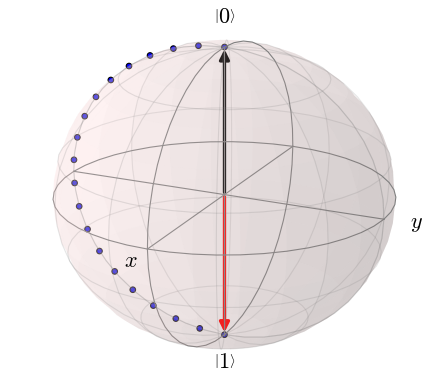
\includegraphics[width=0.6\textwidth]{img/blochxgate.png}
   \caption{Visualization of the X gate on the Bloch sphere. Initial state (black) transformed to final state (red).}
   \label{img:blochxgate}
\end{figure}

From Equ.~\ref{equ:xverification1},~\ref{equ:xverification2} and~\ref{equ:xverification3} it follows that X is its own inverse as well as its own Hermitian conjugate:
\begin{align}
XX &= XX^\dagger = \mathbb{1} \\
X &= X^{-1} = X^\dagger
\end{align}

The action, circuit \& matrix representation and Bloch sphere visualization for the most important single-qubit quantum logic gates are summarised in Table~\ref{tab:singlequbitgates}  below.

\begin{table}[H]
\caption{Table of major single-qubit quantum logic gates.}\vspace{1em}
\label{tab:singlequbitgates}
\begin{tabular}{ C{0.3cm}  C{2cm}  C{1.5cm}  C{1.5cm} C{2.5cm} C{2cm} C{3.5cm}}\hline
Gate & Name & Circuit representation & Matrix & Description & Rotation & Bloch sphere \\ \midrule
$\mathbb{1}$ & Identity & 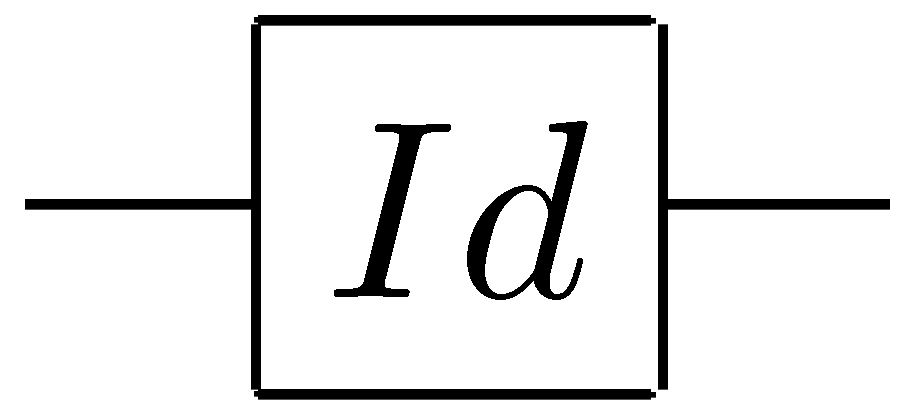
\includegraphics[width=0.1\textwidth]{img/identitycircuit.png} & $\begin{pmatrix}
 1 & 0 \\ 
 0 & 1
 \end{pmatrix}$ & Idle or waiting gate & - & - \\\midrule
X & Qubit flip & 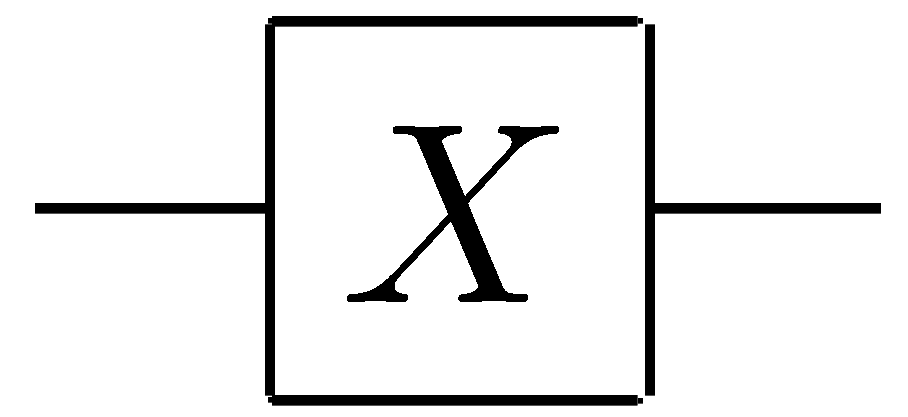
\includegraphics[width=0.1\textwidth]{img/xcircuit.png}  & $\begin{pmatrix}
 0 & 1 \\ 
 1 & 0
 \end{pmatrix}$ & Swaps amplitudes of \0 and \1 & $\pi$ rotation around $\hat{x}$ & 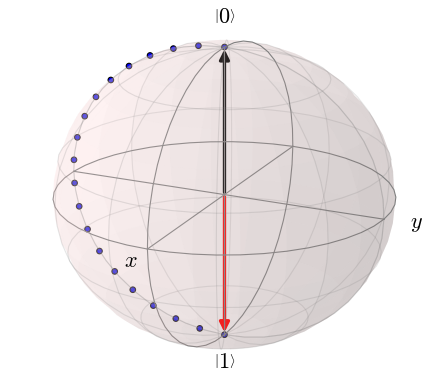
\includegraphics[width=0.2\textwidth]{img/blochxgate.png}\\\midrule
Y & Qubit \& phase flip & 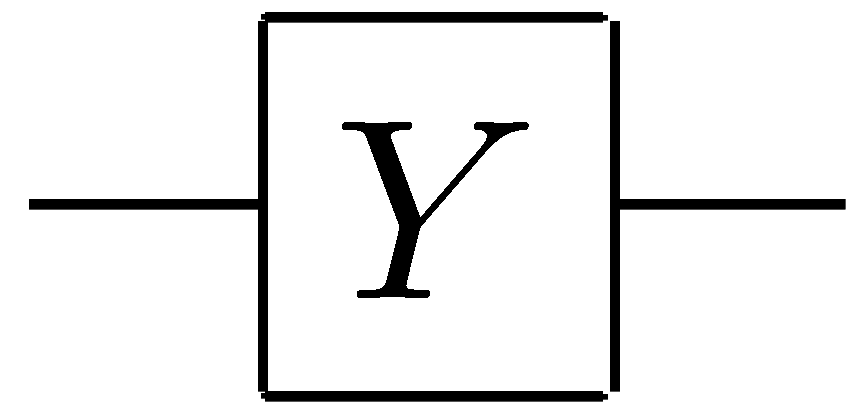
\includegraphics[width=0.1\textwidth]{img/ycircuit.png}  & $\begin{pmatrix}
 0 & -i \\ 
 i & 0
 \end{pmatrix}$ & Swaps amplitudes and introduces phase & $\pi$ rotation around $\hat{y}$ &  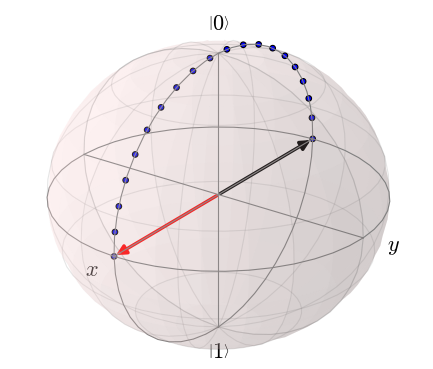
\includegraphics[width=0.2\textwidth]{img/blochygate.png}\\\midrule
Z & Phase flip & 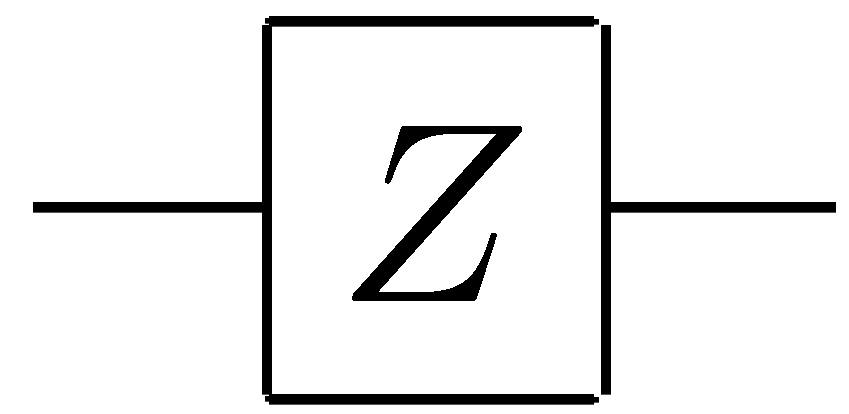
\includegraphics[width=0.1\textwidth]{img/zcircuit.png} & $\begin{pmatrix}
 1 & 0 \\ 
 0 & -1
 \end{pmatrix}$ & Adds a negative sign to the \1 state & $\pi$ rotation around $\hat{z}$ & 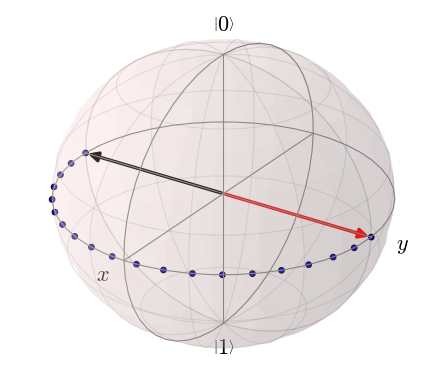
\includegraphics[width=0.2\textwidth]{img/blochzgate.png} \\\midrule 
H & Hadamard & 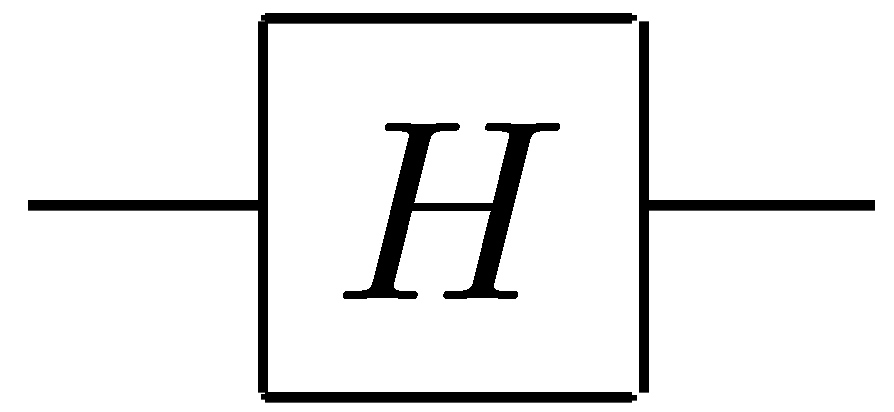
\includegraphics[width=0.1\textwidth]{img/hcircuit.png}  & $\begin{pmatrix}
 \frac{1}{\sqrt{2}} & \frac{1}{\sqrt{2}} \\ 
 \frac{1}{\sqrt{2}} & -\frac{1}{\sqrt{2}}
 \end{pmatrix}$ & Creates equal superpositions & $\frac{\pi}{2}$ rotation around $\hat{y}$ and $\pi$ rotation around $\hat{x}$ & 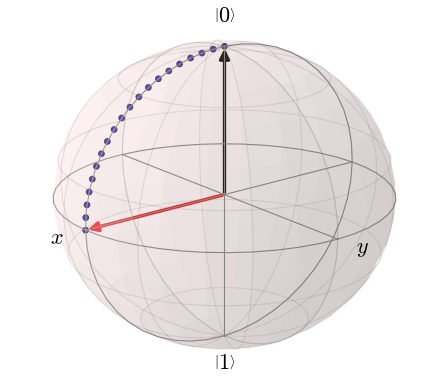
\includegraphics[width=0.2\textwidth]{img/blochhadamard.png}\\\midrule
S & $\frac{\pi}{2}$ rotation gate & 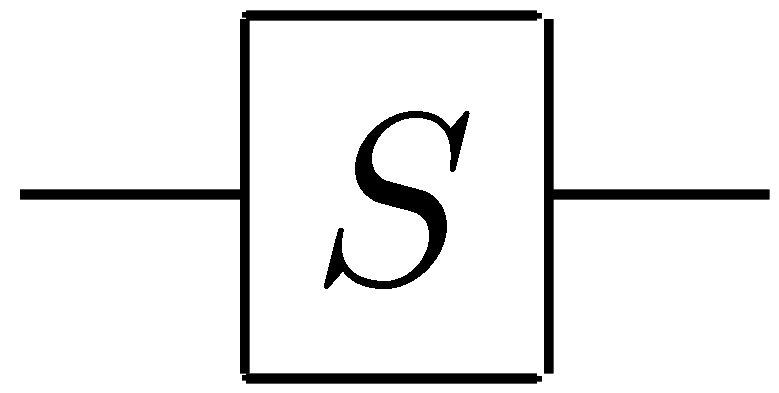
\includegraphics[width=0.1\textwidth]{img/scircuit.png} & $\begin{pmatrix}
 1 & 0 \\ 
 0 & i
 \end{pmatrix}$ & $\sqrt{Z}$ & $\frac{\pi}{2}$ rotation around $\hat{z}$ &  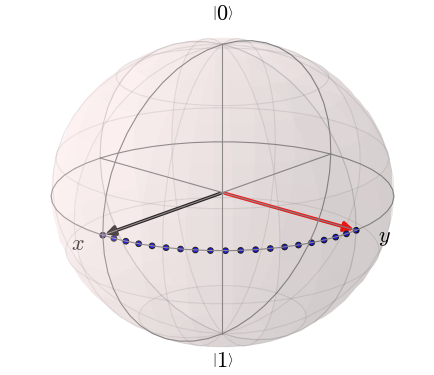
\includegraphics[width=0.2\textwidth]{img/blochsgate.png}\\\midrule
S$^\dagger$ & $-\frac{\pi}{2}$ rotation gate & 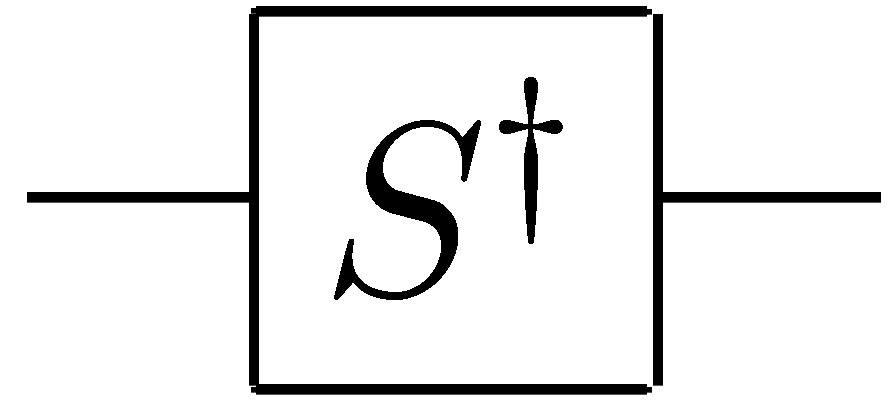
\includegraphics[width=0.1\textwidth]{img/sdcircuit.png} &  $\begin{pmatrix}
 1 & 0 \\ 
 0 & -i
 \end{pmatrix}$ & Adjoint of S & $-\frac{\pi}{2}$ rotation around $\hat{z}$ & \\\midrule
T & $\frac{\pi}{4}$ rotation gate & 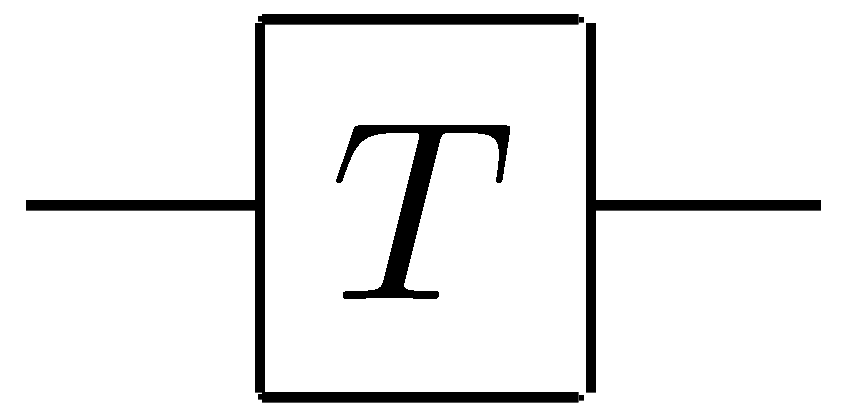
\includegraphics[width=0.1\textwidth]{img/tcircuit.png} & $\begin{pmatrix}
 1 & 0 \\ 
 0 & e^{\frac{i\pi}{4}}
 \end{pmatrix}$ & $\sqrt{S}$ & $\frac{\pi}{4}$ rotation around $\hat{z}$ & 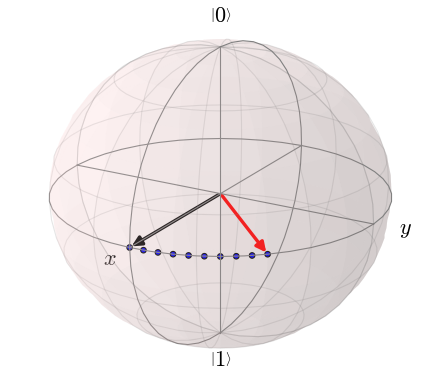
\includegraphics[width=0.2\textwidth]{img/blochtgate.png}\\\midrule
T$^\dagger$ & $-\frac{\pi}{4}$ rotation gate & 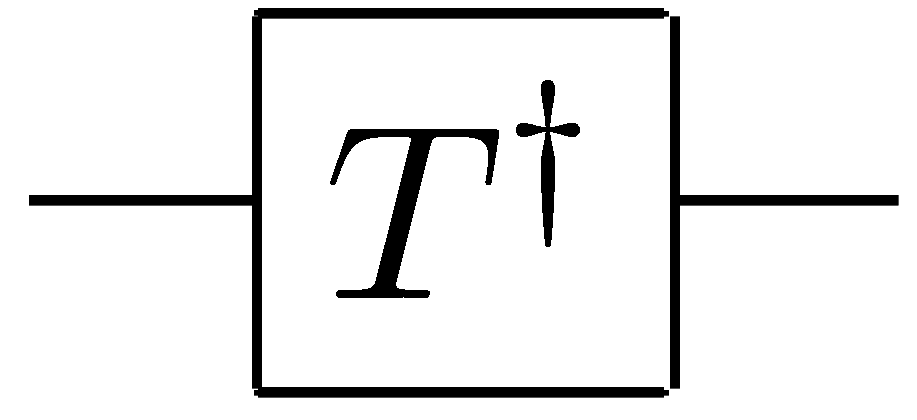
\includegraphics[width=0.1\textwidth]{img/tdcircuit.png} & $\begin{pmatrix}
 1 & 0 \\ 
 0 & e^{-\frac{i\pi}{4}}
 \end{pmatrix}$ & Adjoint of T & $-\frac{\pi}{4}$ rotation around $\hat{z}$ & \\\midrule
ZM & Z-basis measurement & 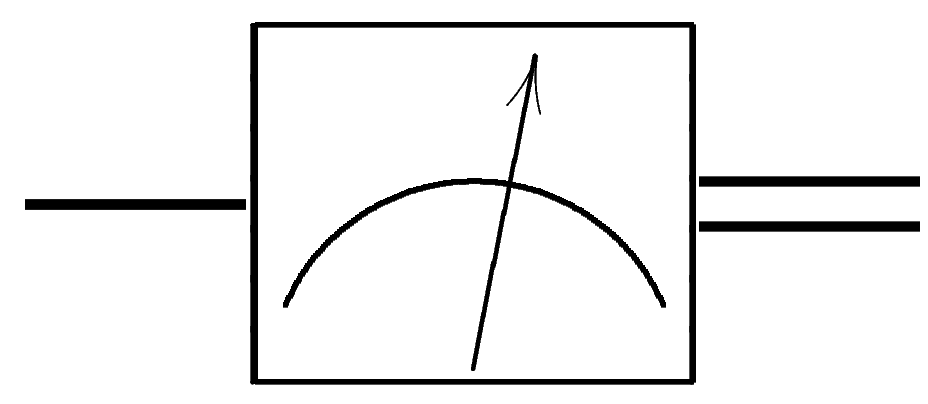
\includegraphics[width=0.1\textwidth]{img/measurecircuit.png} & - & Measurement in standard basis & Collapses the state & - \\
%\midrule
%BM & Bloch measurement & 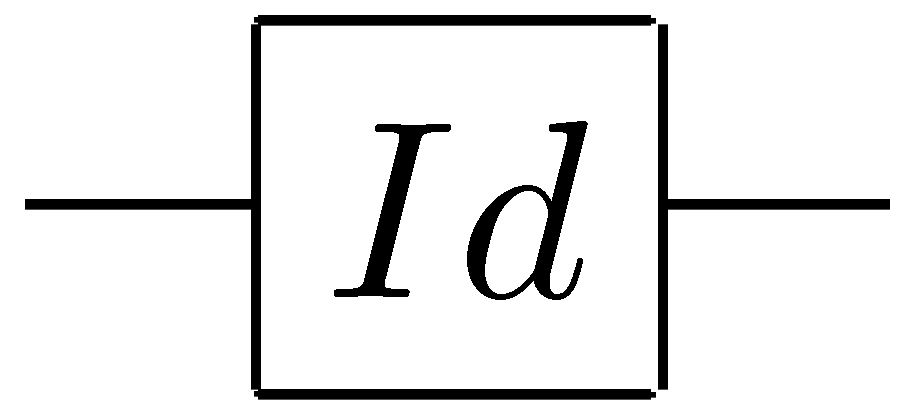
\includegraphics[width=0.1\textwidth]{img/identitycircuit.png} & - & Quantum state tomography & Collapses the state  & -\\
\end{tabular}
\end{table}


%%%%% SUBSECTION: MULTIPLE Q LOGIC GATES


\subsection{Multi qubit gates}
\label{subsubsec:multiqubitgates}

\subsubsection{Controlled-NOT gate}
\label{subsubsubsec:cnotgate}

The most important two-qubit quantum gate is the controlled NOT or CNOT gate given by the following 4x4 matrix:
\begin{equation}
CNOT = \begin{pmatrix}
 \mathbb{1} & 0 \\ 
 0 & X
 \end{pmatrix} = \begin{pmatrix}
 1 & 0 & 0 & 0 \\ 
 0 & 1 & 0 & 0 \\
 0 & 0 & 0 & 1 \\
 0 & 0 & 1 & 0 \\
 \end{pmatrix}
\end{equation}

The CNOT gate takes two qubits, a control and a target qubit, as input. If and only if the control qubit is in the \1 state, the NOT (X) gate is applied to the target qubit. In equations, the CNOT will always be followed by parantheses containing the control (c) qubit followed by the target (t) qubit: CNOT(c,t). The input-output relation (truth table) for the CNOT gate is given in Table~\ref{tab:cnottruthtable} below.

\begin{table}[H]
\begin{center}
\caption{CNOT truth table with first qubit as control, second qubit as target.}\vspace{1ex}
\label{tab:cnottruthtable}
\begin{tabular}{llccc}\hline
Input & Output \\ \hline
00 & 00 \\
01 & 01 \\
10 & 11 \\
11 & 10 \\ \hline
\end{tabular}
\end{center}
\end{table}

To demonstrate the usefulness of the CNOT gate consider starting with two unentangled qubits both in the \0 state,

\begin{equation}
\ket{\phi} = \ket{0} \otimes \ket{0} = \ket{00}
\end{equation}

Applying the H gate onto the first qubit yields the following (still unentangled) state:

\begin{equation}
(H \otimes \mathbb{1}) \ket{\phi} = (H \otimes \mathbb{1}) \ket{00} = \frac{1}{\sqrt{2}} \ket{00} + \frac{1}{\sqrt{2}} \ket{10} 
\end{equation}

Now consider applying the CNOT to this state whereby the control qubit is coloured \textcolor{red}{red} and the target qubit \textcolor{green}{green}.

\begin{equation}
\label{equ:cnotexamples}
CNOT(\textcolor{red}{0},\textcolor{green}{1}) \otimes (\frac{1}{\sqrt{2}} \ket{\textcolor{red}{0}\textcolor{green}{0}} + \frac{1}{\sqrt{2}} \ket{\textcolor{red}{1}\textcolor{green}{0}}) = \frac{1}{\sqrt{2}} \ket{\textcolor{red}{0}\textcolor{green}{0}} + \frac{1}{\sqrt{2}} (\mathbb{1} \otimes X) \ket{\textcolor{red}{1}\textcolor{green}{0}} = \frac{1}{\sqrt{2}} \ket{\textcolor{red}{0}\textcolor{green}{0}} + \frac{1}{\sqrt{2}} \ket{\textcolor{red}{1}\textcolor{green}{1}}
\end{equation}

The last expression in Equ.~\ref{equ:cnotexamples} was used as an example (Equ.~\ref{equ:2qubitnonfactorized}) for entanglement in Section~\ref{subsec:multiqubitsystems} and it is one of the famous Bell states which are a set of four maximally entangled states (CITATION). Thus, this example demonstrates how the CNOT gate is crucial for the generation of entangled states since it applies the X gate to a qubit depending on the state of a second qubit.

The three most important multi qubit quantum gates CNOT, Toffoli and nCNOT are characterised in Table~\ref{tab:multiqubitgates}.

\begin{table}[H]
\caption{Table of major multi-qubit quantum logic gates where $c_j$ stands for the j\textsuperscript{th} control qubit and $\mathbb{1}_k$ for the kxk identity matrix.}\vspace{1em}
\label{tab:multiqubitgates}
\begin{tabular}{ c  C{1.8cm}  C{2cm}  c C{3cm}}\hline
Gate & Name & Circuit representation & Matrix & Description \\ \midrule
CNOT & Controlled NOT & 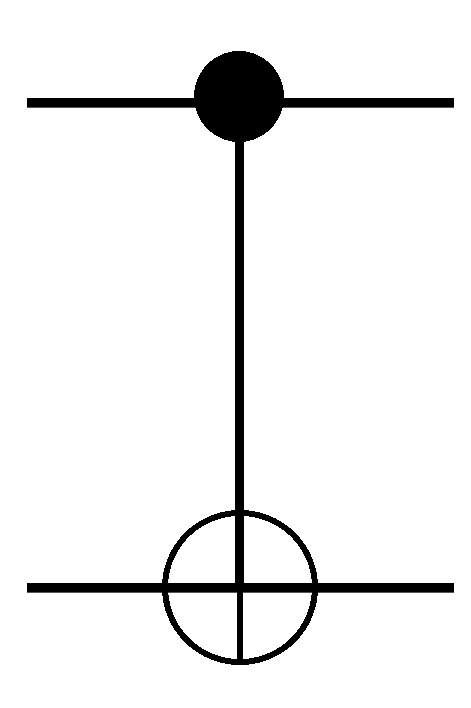
\includegraphics[width=0.1\textwidth]{img/cnotcircuit.png} & $\begin{pmatrix}
 \mathbb{1} & 0 \\ 
 0 & X
 \end{pmatrix} = \begin{pmatrix}
 1 & 0 & 0 & 0 \\ 
 0 & 1 & 0 & 0 \\
 0 & 0 & 0 & 1 \\
 0 & 0 & 1 & 0 \\
 \end{pmatrix}$ & CNOT($c_1$, target) \\\midrule
Toffoli & Controlled controlled NOT & 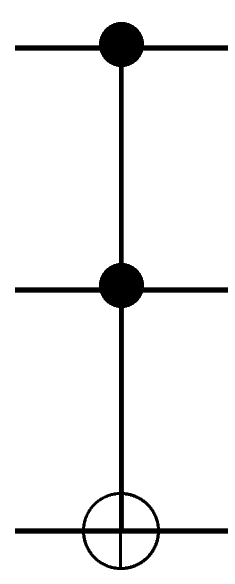
\includegraphics[width=0.1\textwidth]{img/ccnotcircuit.png}  & $\begin{pmatrix}
 \mathbb{1}_6 & 0 \\ 
 0 & X
 \end{pmatrix} = \begin{pmatrix}
 1 & 0 & 0 & 0 & 0 & 0 & 0 & 0 \\ 
 0 & 1 & 0 & 0 & 0 & 0 & 0 & 0 \\ 
 0 & 0 & 1 & 0 & 0 & 0 & 0 & 0 \\ 
 0 & 0 & 0 & 1 & 0 & 0 & 0 & 0 \\ 
 0 & 0 & 0 & 0 & 1 & 0 & 0 & 0 \\ 
 0 & 0 & 0 & 0 & 0 & 1 & 0 & 0 \\
 0 & 0 & 0 & 0 & 0 & 0 & 0 & 1 \\ 
 0 & 0 & 0 & 0 & 0 & 0 & 1 & 0 \\ 
 \end{pmatrix}$ & CCNOT($c_1$, $c_2$, target)\\\midrule
nCNOT & n-controlled NOT & -  & $\begin{pmatrix}
 \mathbb{1}_{2^n-2} & 0 \\ 
 0 & X
 \end{pmatrix}$ & nCNOT($c_1$,..,$c_n$, target) \\\midrule

\end{tabular}
\end{table}

%%%%% SECTION: MACHINE LEARNING

\section{Classical machine learning}
\label{subsec:classicalmachinelearning}

Machine learning (ML), a subfield of artificial intelligence, is aiming to enable computers to learn from data without a human explicitly programming its actions. It can be subdivided into the three major fields supervised \& unsupervised machine learning and reinforcement learning. The three fields can be most easily understood by considering the following three colloquial sentences:

\begin{redbox}
Supervised ML\\
- Based on \emph{input} and \emph{output} data\\
"I know how to classify this data but I need an algorithm to do the computations for me."
\end{redbox}
\begin{greenbox}
Unsupervised ML\\
- Based on \emph{input} data only\\
"I have no clue how to classify this data, can the algorithm create a classifier for me?"
\end{greenbox}
\begin{bluebox}
Reinforcement learning\\
- Based on \emph{input} data only\\
"I have no clue how to classify this data, can the algorithm classify this data and I'll give it a reward if it's correct or I'll punish it if it's not."
\end{bluebox}

This thesis, specifically, is focusing on quantum-enhancements in the field of supervised machine learning only. The following section will introduce a well-known algorithm from the subfield of supervised ML: the $k$-nearest neighbour algorithm.

\subsection{Classical $k$-nearest neighbour algorithm}
\label{subsubsec:knearestneighbour}

Understanding the quantum version of the distance weighted $k$-nearest neighbour (kNN) algorithm as proposed by \citeA{Schuld2014} requires prior knowledge of the classical version of the algorithm that will be introduced in this subsection.

Imagine working for a search engine company and you are given the task of classifying unknown pictures of fruits as either apples or bananas. To train your classification algorithm you are given 5 different pictures of apples and 5 different pictures of bananas. This will be called the \emph{training data set} ${D}_{T}$. The pictures in ${D}_{T}$ may be taken from different angles, in varying light settings and include different coloured apples and bananas. Two examples of such pictures are shown in Fig.~\ref{img:appleandbanana}. 

\begin{figure}[H]
  \begin{minipage}[t]{0.48\textwidth}
    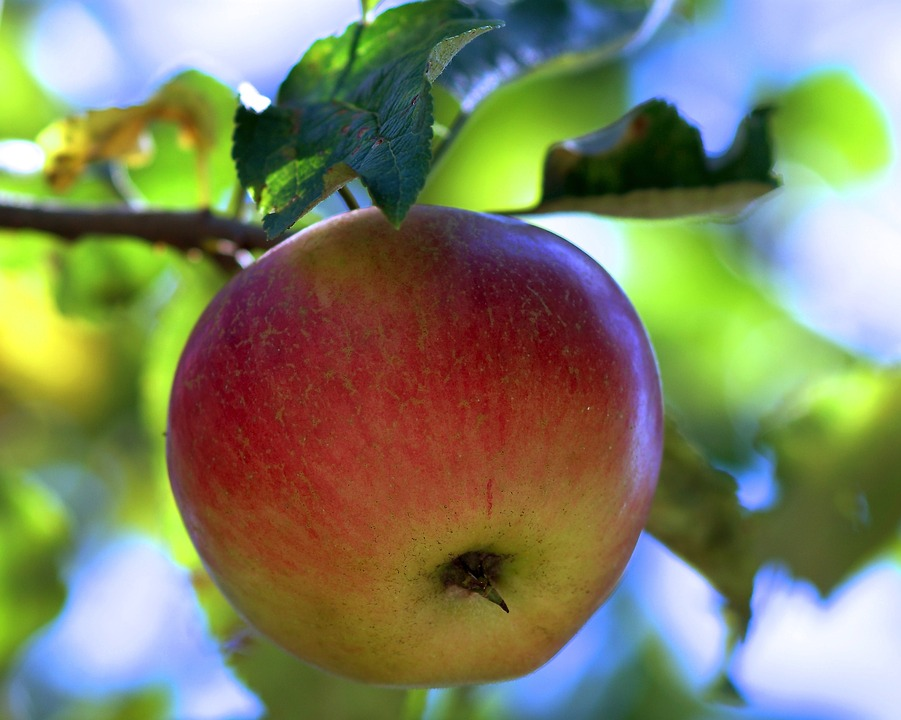
\includegraphics[width = \textwidth]{img/apple.jpg}
  \end{minipage}
  \hfill
  \begin{minipage}[t]{0.48\textwidth}
    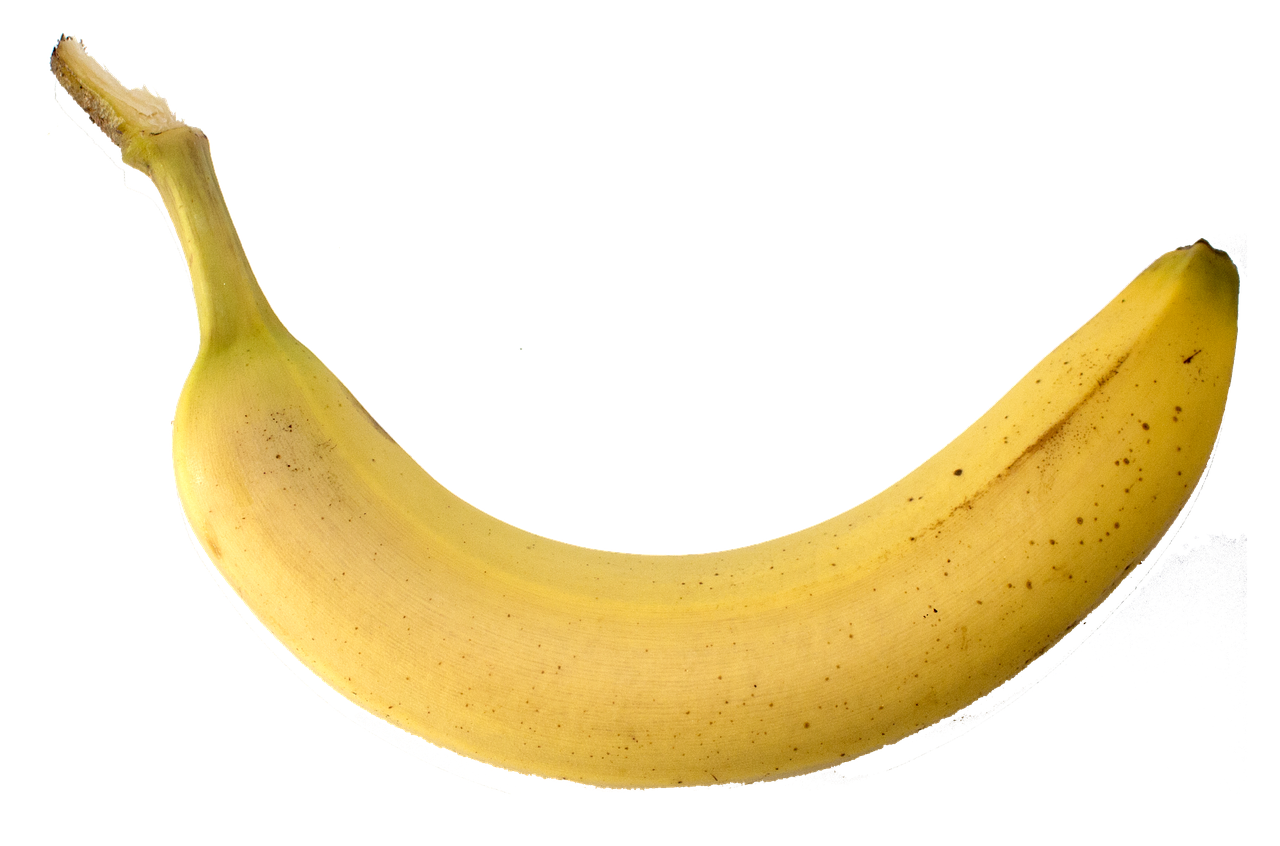
\includegraphics[width = \textwidth]{img/banana.png}
  \end{minipage}
  \caption[]{Pictures of apple and banana from training data set ${D}_{T}$.\footnotemark[3]}
  \label{img:appleandbanana}
\end{figure}

\footnotetext[3]{Reprinted from Pixabay, Retrieved December 24, 2016, from \url{https://pixabay.com/en/apple-red-fruit-frisch-vitamins-1632016/} and \url{https://pixabay.com/en/banana-fruit-yellow-1504956/}. Creative Commons Licence 2016 by Pixabay. Reprinted with permission.}

Most of the time, using the full pixel representation of each picture for classification does not lead to optimal results. Therefore, the next step is to select a certain number of characteristic \emph{features} extracted from the pictures in the training set that can be used to differentiate apples from bananas. Such a feature might be the RGB value of the most frequent pixel colour since bananas and apples have different colour spectra. Using a measure of the curvature of the main object in the picture is another possibility since an apple is almost spherical whereas a banana looks more like a bend line.

By selecting and extracting features, the dimensionality of the training data set is drastically reduced from a few thousand pixels to a handful of features. The $m$ extracted features for the j\textsuperscript{th} picture are stored in the $m$-dimensional \emph{feature vector} $\vec{v}_{j}$. Mathematically, the training data set ${D}_{T}$ consists of ten feature vectors $\vec{v}_{0}, \vec{v}_{1},..,\vec{v}_{10}$ that are each assigned to either class $A$ (apple) or $B$ (banana). The training vectors are visualized as yellow and purple circles in Fig.~\ref{fig:knnconcept}.

Given a new picture of either a banana or an apple, you first extract the same $m$ features from it and store it in the input vector $\vec{x}$. From many algorithms you decide to use the kNN algorithm since it is a non-parametric classifier meaning it makes no prior assumption about the class of the new picture. Given a new unclassified input vector $\vec{x}$ (red star in Fig.~\ref{fig:knnconcept}), the algorithm considers the $k$ nearest neighbours within the training set (using a predefined measure of distance) and classifies $\vec{x}$, based on a majority vote, as either $A$ or $B$. Thereby, $k$ is a positive integer, usually chosen to be small and its value determines the classification outcome. Namely, in the case $k = 3$ in Fig.~\ref{fig:knnconcept}, vector $\vec{x}$ will be classified as class B (purple) but in the case $k = 6$ it will be labelled class A (yellow).

\begin{figure}[H]
      \centering
       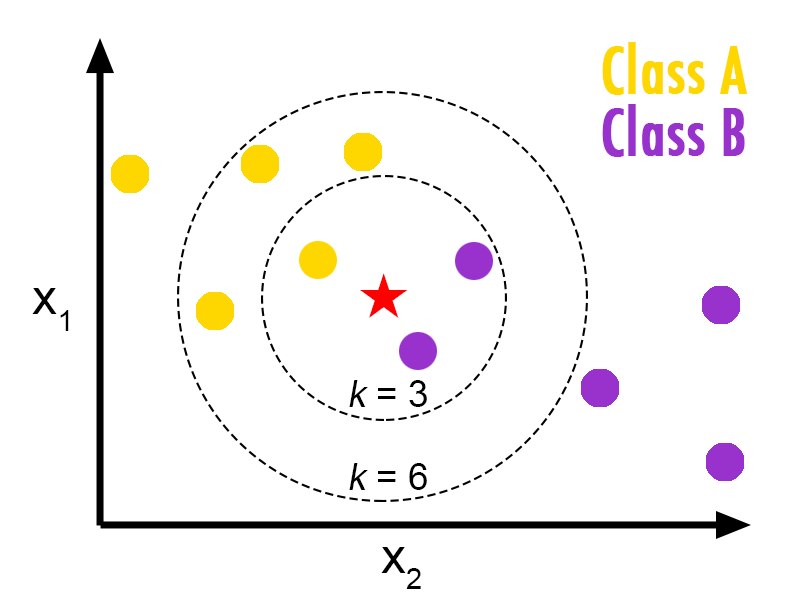
\includegraphics[scale=0.8]{img/knn-concept.png}
       \caption[]{\label{fig:knnconcept} Visualization of a kNN classifier\footnotemark[4]}
\end{figure}

\footnotetext[4]{Reprinted from GitHub, Burton de Wilde, Retrieved September 13, 2016, from \url{http://bdewilde.github.io/blog/blogger/2012/10/26/classification-of-hand-written-digits-3/}. Copyright 2012 by Burton de Wilde. Reprinted with permission.}

In the case of $k = 10$, $\vec{x}$ would simply be assigned to the class with the most members. In this case, the training vectors should be given distance-dependent weights (such as $\frac{1}{distance}$) to increase the influence of closer vectors over more distant ones.

\subsection{Algorithmic time complexity}
\label{subsubsec:algcomplexity}

\subsubsection{Big-O notation}
\label{subsubsubsec:bigO}

In the fields of computer science and quantum information, the so-called Big-O notation, first described by \citeA{bachmann1894analytische}, is often used to describe how the runtime of an algorithm depends on variables such as the desired accuracy, the number of input vectors or their size.

\begin{redbox}
\textbf{Definition: Big-O $\mathcal{O}$}\\
\newline
For any monotonic functions $t(n)$ and $g(n)$ defined on a subset of the real numbers (${\rm I\!R}$), one says that $t(n) = \mathcal{O}(g(n))$ if and only if when there exists constants $c \geq 0$ and $n_0 \geq 0$ such that

\begin{equation}
\mid f(n) \mid \quad \leq \quad c\text{ }*\mid g(n) \mid \quad \text{for all } n \geq n_0
\end{equation}
\end{redbox}
\begin{redbox}
\begin{figure}[H]
      \centering
       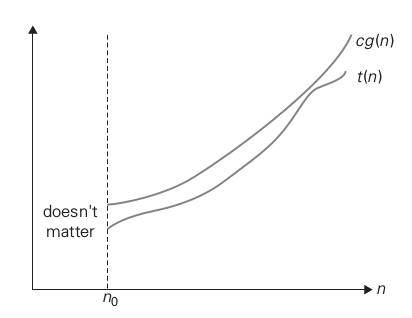
\includegraphics[scale=0.3]{img/asymptoticupperbound.png}
       \caption[]{\label{fig:upperasym} Visualization of $c\text{ }*g(n)$ being an upper asymptotic bound of $t(n)$\footnotemark[5]}
\end{figure}

\footnotetext[5]{Reprinted from Anany Levitin and Soumen Mukherjee. Introduction to the Design \& Analysis of Algorithms. Reading, MA: Addison-Wesley, 2003. Copyright 2012 by Levitin \& Mukherjee.}

This implies that the function $f(n)$ does not grow at a faster rate than $g(n)$, or in other words that some constant multiple of the function $g(n)$ is an upper asymptotic bound for the function $f(n)$, for all $n\rightarrow \infty$.
\end{redbox}

Fig.~\ref{fig:algcomplexities} provides a good visual comparison between common algorithmic complexity classes regarding their relation to the input size $n$. It can be seen that the best possible algorithmic time complexity is constant time, $\mathcal{O}(1)$, that is being independent of the size of the input data e.g. determining if a binary number is even or odd. An algorithm is still considered excellent if it runs in logarithmic time $\mathcal{O}(log(n))$. Linear search algorithms for example are linear in time expressed as $\mathcal{O}(n)$. More complex sort algorithms like "bubble sort" have a higher time complexity and often run in quadratic time ($\mathcal{O}(n^2)$). Furthermore, algorithms with complexity $\mathcal{O}(n^c)$ are said to run in polynomial time for some $c > 2$. If an algorithm has time complexity $\mathcal{O}((log(n))^c)$ for some $c \geq 1$ it is called polylogarithmic. The highest complexity classes are exponential $\mathcal{O}(c^n)$ with $c \geq 1$ and factorial time $\mathcal{O}(n!)$. For example, solving the travelling salesman problem using brute-force search runs in factorial time.

\begin{figure}[H]
      \centering
       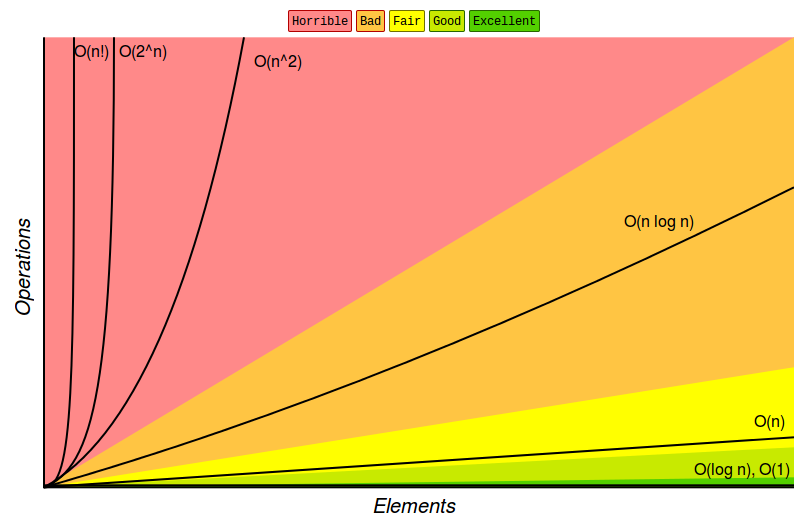
\includegraphics[scale=0.35]{img/bigocomplexity.png}
       \caption[]{\label{fig:algcomplexities} Overview of algorithmic complexity classes\footnotemark[6]}
\end{figure}
\footnotetext[6]{Reprinted from Big-O Cheatsheet, Retrieved December 28, 2016, from \url{http://bigocheatsheet.com/}. Copyright 2016 by Big-O Cheatsheet. Reprinted with permission.}

\chapter{Methods}\label{sec:methods}

The entirety of the research for this thesis is performed with pen and paper and a computer running the Linux operating system Ubuntu. The programming language Python, with its very intuitive syntax and large libraries for scientific computing and plotting, was used for the calculations and most of the plots for this thesis. More specifically, the open-source QuTiP library\footnotemark[7] for Python was used to create the Bloch sphere plots. All function plots were embedded directly into \LaTeX  by using the pgfplots package\footnotemark[8].

\footnotetext[7]{The open-source QuTiP library for Python may be downloaded from \url{http://qutip.org/}.}
\footnotetext[8]{The \LaTeX  pgfplots package may be downloaded from \url{https://www.ctan.org/pkg/pgfplots}.}

For the implementation of the quantum kNN algorithm there are two fundamentally different ways: Running it a) by simulating a QC or b) by actually executing it on a real QC. The required tools for both possibilities will be explained in the following subsections.

\section{Liqui$\ket{}$}
\label{subsec:simulation}

Classical computers can be used to simulate the behaviour of small quantum computers. Such simulations are associated with exponential computational costs thereby limiting the number of simulated qubits. Since current state-of-the-art quantum technology uses around ten qubits, a classical computer can still be used for simulation.

For the quantum computing simulations in this thesis the quantum simulation toolsuite Liqui$\ket{}$ developed by \citeA{liquid} will be used. Liqui$\ket{}$ is based on the functional programming language F\# and allows for simulation of up to 30 qubits \cite{microsoftresearch}. It comes with a large palette of predefined single and multi qubit quantum logic gates and allows for custom-defined quantum gates such as nCNOT and rotation gates controlled by $n$ qubits which is crucial for some of the work done in this thesis. A short piece of example code from Liqui$\ket{}$ written in F\# is shown in Fig.~\ref{fig:liquidsnippet}. For all quantum simulations in this thesis, a Lenovo ThinkPad T450 with an Intel i5 processor (2 cores) and 8GB random-access memory (RAM) is used.

\begin{figure}[H]
      \centering
       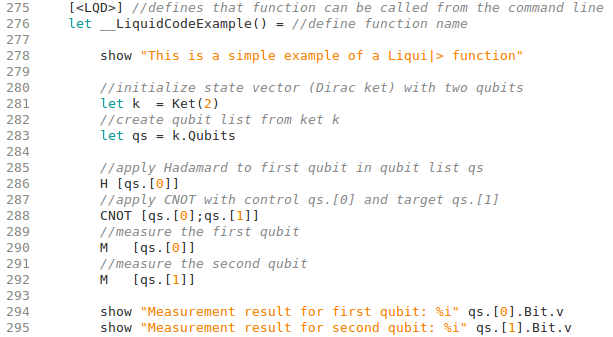
\includegraphics[scale=0.65]{img/liquidcodesnippet.png}
       \caption{\label{fig:liquidsnippet} F\# code snippet from Microsoft's quantum simulation toolsuite Liqui$\ket{}$}
\end{figure}

\section{IBM Quantum Experience}
\label{subsec:ibmqc}

Earlier this year IBM has enabled public cloud access to their experimental quantum processor containing five non error-corrected superconducting qubits located at the IBM Quantum Lab at the Thomas J Watson Research Center in Yorktown Heights, New York \cite{ibmquantumcomputer}. Instead of only simulating on classical hardware, this opens up the possibility of executing the QML algorithm on actual quantum hardware.

The so-called IBM Quantum Experience\footnotemark[9] provides the user with access to their \emph{quantum composer} which is the main tool for algorithm design. The quantum composer shown in Fig.~\ref{fig:composer} consists of 5 horizontal lines, one for each qubit, and enables the user to choose from a universal gate set (bottom of Fig.~\ref{fig:composer}) consisting of the following 10 quantum logic gates: $\mathbb{1}$, X, Y, Z, H, S, S$^\dagger$, T, T$^\dagger$ and CNOT. Additionally, there are two different types of measurement: a) A measurement in the standard z-basis ($\ket{0}$ / $\ket{1}$) resulting in a probability distribution over all possible states and b) a Bloch measurement that visually projects the state onto the Bloch sphere. The user can compose an algorithm by applying up to 40 quantum logic and measurement gates to the five qubits by means of drag-and-drop.
\footnotetext[9]{The IBM Quantum Experience can be accessed via \url{https://quantumexperience.ng.bluemix.net/qstage/}.}

\begin{figure}[H]
      \centering
       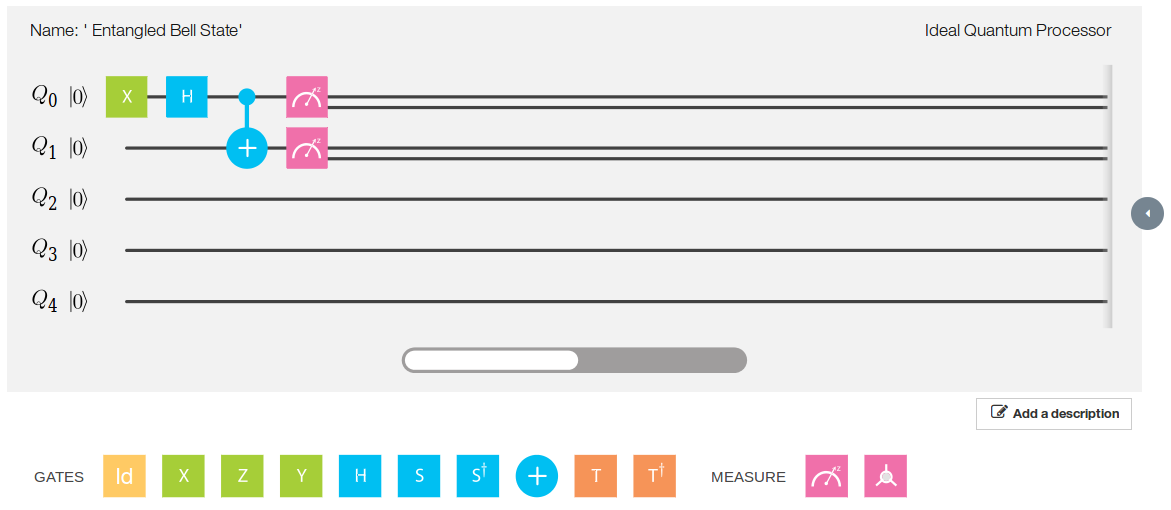
\includegraphics[scale=0.36]{img/ibmcomposer.png}
       \caption[]{\label{fig:composer} Screenshot showing IBM Quantum Composer\footnotemark[10]}
\end{figure}
\footnotetext[10]{Screenshot was taken from \url{https://quantumexperience.ng.bluemix.net/qstage/#/editor}.}

By spending limited user coins the gate sequence of a composed algorithm is then send to IBM's QC in New York and depending on the waiting queue and the availability of the QC the results will be sent back via mail within a few minutes or days. IBM Quantum Experience also allows for free quantum simulations under ideal or real conditions which provides a great tool for experimentation without spending user coins.

The main limitation of the IBM Quantum Experience are the qubit decoherence times since they restrict the maximum number of possible operations before the qubits lose their quantum behaviour and their quantum information. Thus, the number of quantum gates is currently limited to only 40 which essentially means 39 logic gates and 1 measurement gate. According to the qubit calibration results shown in Fig.~\ref{fig:calibration}, the amplitude damping times of the five qubits range from \SI{52.3}{\micro\second} to \SI{81.5}{\micro\second}. Furthermore, the phase damping times range from \SI{60.9}{\micro\second} to \SI{112.4}{\micro\second}. Currently, the implementation of a single qubit quantum logic gate takes 130ns and applying a CNOT gate takes 500ns \cite{ibmgatetimes}.

\begin{figure}[H]
      \centering
       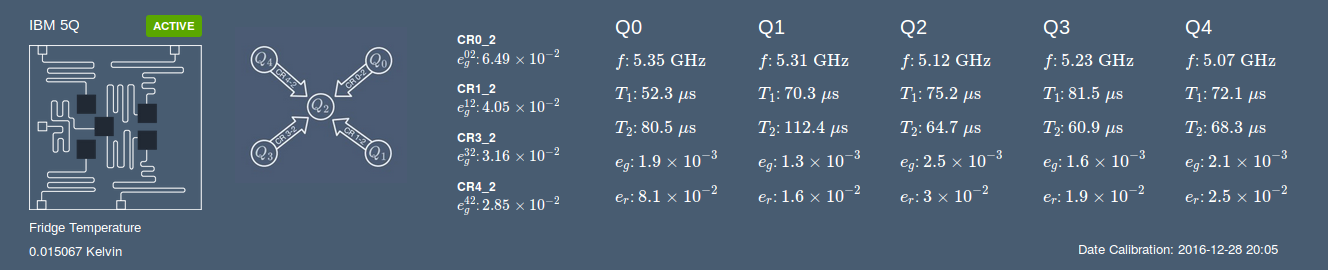
\includegraphics[scale=0.33]{img/ibmcalibration.png}
       \caption[]{\label{fig:calibration} Screenshot of IBM QC calibration results (28. December 2016 - 20:05)\footnotemark[11]}
\end{figure}
\footnotetext[11]{Screenshot was taken from \url{https://quantumexperience.ng.bluemix.net/qstage/#/editor}.}

\chapter{Literature Review: Quantum-enhanced Machine Learning}\label{sec:qml}

Classical machine learning takes classical data as input and learns from it using classical algorithms executed on classical computers - this will be referred to as C/C (classical data with classical algorithm). One enters the field of quantum machine learning when either quantum data or quantum algorithms are combined with ideas from classical machine learning. Thus, quantum machine learning can be subdivided into three different subfields: 1) C/Q - classical data with quantum algorithm, 2) Q/C - quantum data with classical algorithm and 3) Q/Q - quantum data with quantum algorithm.

\emph{Quantum data} includes any data describing a quantum mechanical system such as e.g. the Hamiltonian of a system or the state vector of a certain quantum state. A \emph{quantum algorithm} is any algorithm that can be executed on a quantum computer only. 

The subfield Q/C processes quantum data with classical machine learning algorithms e.g. \citeA{las2016genetic} made use of classical genetic algorithms to improve the experimental and digital errors in quantum gates. Subfield Q/Q  is the union of C/Q and Q/C and deals with the processing of quantum data using quantum algorithms e.g. learning the Hamiltonian of a quantum system using quantum machine learning algorithms.

The topic of this thesis is embedded within the subfield C/Q that aims to develop quantum algorithms for machine learning tasks involving classical data. This subfield is also called \emph{quantum-enhanced machine learning} since clever algorithm design can harness quantum parallelism to speed-up classical machine learning algorithms. The following sections will introduce main concepts from the field of quantum-enhanced machine learning. More specifically, Section~\ref{subsubsec:quantumstatepreparation} will outline how classical data can be transferred into quantum states and Section~\ref{subsubsec:quantumknearestneighbour} introduces a quantum version of the classical $k$-nearest neighbour algorithm.

\newpage
\section{Quantum state preparation}
\label{subsec:quantumstatepreparation}

\emph{Quantum state preparation} is the process of preparing a quantum state that accurately represents a vector containing classical (normalized) data. There are two fundamentally different ways of preparing a quantum state representing the classical example vector v:
\begin{equation}
\label{equ:v}
v = \begin{pmatrix}0.6 \\ 0.4 \end{pmatrix}
\end{equation}

\subsection{Encoding classical data into qubits}
\label{subsubsec:classicaldataqubits}
%speed-up not very clear since the \# of qubits increases linearly with the \# of classical bits
The most straightforward type of quantum state preparation does not make use of quantum superpositions but only uses the definite \0 or \1 states to store binary information in a multi qubit system as outlined in the example below.

Multiply vector v by ten such that the normalized entries can easily be represented in binary,
\begin{equation}
\begin{pmatrix}
 \textcolor{blue}{0.6} \\ 
 \textcolor{emerald}{0.4}
 \end{pmatrix}*10 = \begin{pmatrix}
 \textcolor{blue}{6} \\ 
 \textcolor{emerald}{4}
 \end{pmatrix}
\end{equation}
 Convert each entry to binary,
 \begin{equation}
 \begin{pmatrix}
 \textcolor{blue}{6} \\ 
 \textcolor{emerald}{4}
 \end{pmatrix} \rightarrow \begin{pmatrix}
 \textcolor{blue}{0110} \\ 
 \textcolor{emerald}{0100}
 \end{pmatrix}
 \end{equation}
 Rewrite the 2-D vector as a 1-D bit string,
 \begin{equation}
 \begin{pmatrix}
 \textcolor{blue}{0110} \\ 
 \textcolor{emerald}{0100}
 \end{pmatrix} \rightarrow n=\textcolor{blue}{0110}\textcolor{emerald}{0100}
\end{equation}
For $g$ bits initialize $g$ qubits in the \0 state \& apply the X gate to the respective qubits:
\begin{equation}
n=\textcolor{blue}{0110}\textcolor{emerald}{0100}  \rightarrow \ket{n} = (\textcolor{blue}{\mathbb{1} \otimes X \otimes X \otimes \mathbb{1}}\otimes\textcolor{emerald}{\mathbb{1} \otimes X \otimes \mathbb{1} \otimes \mathbb{1}})\ket{00000000} = \ket{\textcolor{blue}{0110}\textcolor{emerald}{0100}}
\end{equation}
%\textbf{Only slight speed up possible}
When encoding classical data into qubit states, a $k$-dimensional probability vector requires $4k$ classical bits which are encoded one-to-one into $4k$ qubits. Thus, the number of qubits increases linearly with the size of the classical data vector. Due to this one-to-one correspondence between classical bits and qubits there is no data compression improvement compared to classical data storage.
%Only slight (up to quadratic) speed-ups are possible through clever quantum algorithm design (CITATION).

Qubit-based quantum state preparation becomes slightly more complicated when aiming to achieve a quantum memory state $\ket{M}$ in an equal superposition of $l$ binary patterns $l^j$ of the form:
\begin{equation}
\label{equ:memorysuperpos}
\ket{M} = \frac{1}{\sqrt{l}}\sum^l_{j=1} \ket{l^j}
\text{where } \ket{l^j} = \ket{l^j_1,l^j_2,...l^j_n} \text{and } l^j_k \in \left\{0,1\right\}
\end{equation}
Preparing this quantum state is a requirement for the later used qubit-encoded kNN quantum algorithm by \citeA{Schuld2014}. \citeA{Trugenberger2001} describe a quantum routine that can efficiently prepare such a state as will be explained in detail below.

\pagebreak
First, \citeA{Trugenberger2001} defines the new unitary quantum gate $S^j$,
\begin{equation}
S^j = \begin{pmatrix}
\sqrt{\frac{j-1}{j}} & \frac{1}{\sqrt{j}} \\
-\frac{1}{\sqrt{j}} & \sqrt{\frac{j-1}{j}}
\end{pmatrix}
\end{equation}
and introduces its controlled version $CS^j$:
\begin{equation}
CS^j = \begin{pmatrix}
\mathbb{1} & 0 \\
0 & S^j
\end{pmatrix}
\end{equation}
The initial quantum state is given in Equ.~\ref{equ:truginitial} and consists of three registers; the first being the pattern register containing the first pattern $l^1$, the second register $u$ is a utility register initialized in state $\ket{01}$ and the third register $m$ represents the memory register initialized with $n$ zeros in which all patterns $l^j$ will be loaded one after the other.
\begin{equation}
\label{equ:truginitial}
\ket{\Psi^1_0} = \ket{l^1;u;m} = \ket{l^1_1,l^1_1,...,l^1_n;01;0_1,...,0_n} 
\end{equation}
The routine will use the second utility qubit $u_2$ to separate the intial state into two terms whereby $u_2 = \ket{0}$ flags the already stored patterns and $u_2 = \ket{1}$ indicates the processing term. In order to store a pattern $l^j$ in the memory register one has to perform the following operations:

\begin{bluebox}
Step 1: Using $u_2$ as one of the control qubits for the CCNOT gate, copy the pattern $l^j$ into the memory register of the processing term ($u_2=\ket{1}$):
\begin{equation}
\label{equ:trug1}
\ket{\Psi^j_1} = \prod_{r=1}^n CCNOT(l^j_r,u_2,m_r)\ket{\Psi^j_0} 
\end{equation}

Step 2: If the qubits in the pattern and memory register are identical (true only for the processing term) then overwrite all qubits in the memory register with ones:
\begin{equation}
\label{equ:trug2}
\ket{\Psi^j_2} = \prod_{r=1}^n X(m_r)CNOT(l^j_r,m_r)\ket{\Psi^j_1} 
\end{equation}

Step 3: Apply a nCNOT gate controlled by all $n$ qubits in the $m$ register and flip $u_2$ if and only if all $n$ qubits are ones (true only for the processing term):
\begin{equation}
\label{equ:trug3}
\ket{\Psi^j_3} = nCNOT(m_1,m_2,...,m_n,u_2)\ket{\Psi^j_2} 
\end{equation}

Step 4: Using the previously defined $CS^j$ operation, with control $u_1$ and target $u_2$ , the new pattern is transferred from the processing term into the term containing the already stored patterns ($u_2 = \ket{0}$):
\begin{equation}
\label{equ:trug4}
\ket{\Psi^j_4} = CS^{l+1-j}(u_1,u_2) \ket{\Psi^j_3} 
\end{equation}
\end{bluebox}
\begin{bluebox}
Step 5 \& 6: In Step 2 \& 3 all qubits in the memory register were overwritten with ones and these steps can be undone by applying their inverse operations:
\begin{align}
\label{equ:trug56}
\ket{\Psi^j_5} &= nCNOT(m_1,m_2,...,m_n,u_2)\ket{\Psi^j_4} \\
\ket{\Psi^j_6} &= \prod_{r=n}^1 CNOT(l^j_r,m_r)X(m_r)\ket{\Psi^j_5} 
\end{align}

The resulting state is now given by the following equation:
\begin{equation}
\label{equ:trug6}
\ket{\Psi^j_6} = \frac{1}{\sqrt{l}} \sum^{j}_{w=1} \ket{l^j;00;l^w} + \sqrt{\frac{l-j}{l}} \ket{l^j;01;l^j}
\end{equation}

Step 7: Finally, by applying the inverse operation of Step 1 the memory register of the processing term is restored to zeros only:
\begin{equation}
\label{equ:trug7}
\ket{\Psi^j_7} = \prod_{r=n}^1 CCNOT(l^j_r,u_2,m_r) \ket{\Psi^j_6} 
\end{equation}
\end{bluebox}

At the end of Step 7 the next pattern can be loaded into the first register and by applying Steps 1-7 again the pattern gets added to the memory register. After repeating this procedure $l$ times the memory register $m$ will be in the desired state $\ket{M}$ defined by Equ.~\ref{equ:memorysuperpos}.

\subsection{Encoding classical data into amplitudes}
\label{subsubsec:classicaldataamplitudes}

A more sophisticated way of representing the classical vector $v$ (Equ.~\ref{equ:v}) as a quantum state makes use of the large number of available amplitudes in a multi qubit system. The general idea is demonstrated in Equ.~\ref{equ:amplitudedata} below.
\begin{equation}
\label{equ:amplitudedata}
\begin{pmatrix}
 \textcolor{blue}{0.6} \\ 
 \textcolor{emerald}{0.4}
 \end{pmatrix} \quad \rightarrow \quad \ket{n} = \sqrt{\textcolor{blue}{0.6}}\ket{0}+\sqrt{\textcolor{emerald}{0.4}}\ket{1}
\end{equation}
Using amplitude-based quantum state preparation, a $k$-dimensional probability vector is encoded into only $log_{2}(k)$ qubits since the number of amplitudes grows exponentially with the number of qubits. This type of quantum data storage makes exponential compression of classical data possible. Since a quantum gate acts on all amplitudes in the superposition at once there is the possibility of exponential speed-ups in quantum algorithms compared to their classical counterparts. Compared to the one-to-one correspondence in qubit-encoded state preparation, amplitude-encoding requires a much smaller number of qubits that grows logarithmically with the size of the classical data vector. However, initializing an arbitrary amplitude distribution is still an active field of research and requires the implementation of non-trivial quantum algorithms.

For the case when the classical data vectors represent discrete probability distributions which are efficiently integrable on a classical computer, \citeA{Grover2002} developed a quantum routine to initialize the corresponding amplitude distribution.
%The main idea in their algorithm is subdividing the respective probability distribution and encoding the probabilty
%VERY COMPLICATED AND MOST GENERAL
Additionally, \citeA{soklakov2006efficient} proposed a quantum algorithm for the more general case that includes initializing amplitude distributions for classical data vectors representing non-efficiently integrable probability distributions.

\section{Quantum k-nearest neighbour algorithm}
\label{subsec:quantumknearestneighbour}

The quantum distance-weighted kNN algorithm outlined in this section was proposed by \citeA{Schuld2014} and is based on classical data being encoded into qubits rather than amplitudes. The first step is to prepare an equal superposition $\ket{T}$ over $N$ training vectors $\vec{v}$ of length $n$ with binary entries $v_1,v_2,...v_n$ each assigned to a class $c$ as follows,
\begin{equation}
\label{equ:qubitknninitial}
\ket{T} = \frac{1}{\sqrt{N}}\sum_{p=1}^N \ket{v_1^p,v_2^p,...v_n^p;c^p}
\end{equation}
The unknown vector $\vec{x}$ of length $n$ and binary entries $x_1,x_2,...x_n$ needs to be classified and is added to the training superposition resulting in the initial state $\ket{\psi_0}$:
\begin{equation}
\ket{\psi_0} = \frac{1}{\sqrt{N}}\sum_{p=1}^N \ket{x_1,x_2,...x_n;v_1^p,v_2^p,...v_n^p;c^p}
\end{equation}
An ancilla qubit initially in state \0 is added to the state such that the superposition is now described by,
\begin{equation}
\ket{\psi_1} = \frac{1}{\sqrt{N}}\sum_{p=1}^N \ket{x_1,x_2,...x_n;v_1^p,v_2^p,...v_n^p;c^p} \otimes \ket{0}
\end{equation}
The state now consists of four registers: 1) input($x$) register, 2) training($v$) register, 3) class($c$) register and 4) ancilla($\ket{0}$) register. Next, the ancilla register is put into an equal superposition by applying an H gate to it,
\begin{align}
\ket{\psi_2} &= \frac{1}{\sqrt{N}}\sum_{p=1}^N \ket{x_1,x_2,...x_n;v_1^p,v_2^p,...v_n^p;c^p} \otimes H\ket{0}\notag\\
&= \frac{1}{\sqrt{N}}\sum_{p=1}^N \ket{x_1,x_2,...x_n;v_1^p,v_2^p,...v_n^p;c^p} \otimes \frac{(\ket{0}+\ket{1})}{\sqrt{2}}
\end{align}
The main step in any kNN algorithm is calculating some measure of distance between each training vector $\vec{v}$ and the input vector $\vec{x}$ which in this quantum algorithm is taken to be the Hamming distance defined in the red box below.

\begin{redbox}
\textbf{Definition: Hamming distance}\\
\newline
First defined by \citeA{hamming1950error}, Hamming distance (HD) is the number of differing characters when comparing two equally long binary patterns $p_0$ and $p_1$.\\
\newline
Example:\\
$p_0 = \quad\textcolor{red}{0}\quad\textcolor{emerald}{0\quad1}$\\
$p_1 = \quad\textcolor{red}{1}\quad\textcolor{emerald}{0\quad1}$\\
$--------$\\
HD $= 1+0+0 = 1$
According to \citeA{Trugenberger2001}, HD is the squared Euclidean distance between the two binary patterns $p_0$ and $p_1$.
\end{redbox}

Given quantum state $\ket{\psi_2}$ the HD between the input and each training register can be calculated by applying CNOT($x_s,v_s^p$) gates to all qubits in the first and second register using the input vector qubits $x_s$ as controls and the training vector qubits $v_s^p$ as targets. The sum of the qubits in the second register now represents the total HD between each training register and the input. Applying an X gate to each qubit in the second register reverses the HD such that small HDs become large and vice versa. This is crucial since training vectors close to the input should get larger weights than more distant vectors. This procedure will change the qubits in the second register according to the rules specified in Equ.~\ref{equ:distancerules}. 
\begin{equation}
\label{equ:distancerules}
d^p_s =
    \begin{cases}
      1, & \text{if}\ \ket{v_s^p} = \ket{x_s} \\
      0, & \text{otherwise}
    \end{cases}
\end{equation}
The quantum state is now given by,
\begin{align}
\ket{\psi_3} &= \prod_{s=1}^n X(v^p_s)CNOT(x_s,v^p_s)\ket{\psi_2}\notag\\
&= \frac{1}{\sqrt{N}}\sum_{p=1}^N \ket{x_1,x_2,...x_n;d_1^p,d_2^p,...d_n^p;c^p} \otimes \frac{(\ket{0}+\ket{1})}{\sqrt{2}}
\end{align}
By applying the unitary operator $U$ defined by,
\begin{equation}
\label{equ:sumoperator}
U = e^{-i\frac{\pi}{2n}K}
\end{equation}
where
\begin{equation}
\label{equ:sumoperator2}
K = \mathbb{1} \otimes \sum_s (\frac{\sigma_z+1}{2})_{d_s} \otimes \mathbb{1} \otimes (\sigma_z)_c
\end{equation}
the sum over the second register is computed. As a result, the total reverse HD, denoted $d_H(\vec{x},\vec{v}^p)$, between the $p$th training vector $\vec{v}^p$ and the input vector $\vec{x}$ is written into the complex phase of the p$th$ term in the superposition. The ancilla register is now separating the superposition into two terms due to a sign difference in the amplitudes (negative sign when ancilla is \1). The result is given by, 
\begin{align}
\ket{\psi_4} &= U\ket{\psi_3}\notag\\
&= \frac{1}{\sqrt{2N}}\sum_p^N e^{i\frac{\pi}{2n}d_H(\vec{x},\vec{v}^p)} \ket{x_1,x_2,...x_n;d_1^p,d_2^p,...d_n^p;c^p;0} \notag\\
&\quad\quad\quad\quad\quad\quad + e^{-i\frac{\pi}{2n}d_H(\vec{x},\vec{v}^p)} \ket{x_1,x_2,...x_n;d_1^p,d_2^p,...d_n^p;c^p;1}
\end{align}
Applying an H gate to the ancilla register transfers the $d_H(\vec{x},\vec{v}^p)$ from the phases into the amplitudes such that the new quantum state is described by,
\begin{align}
\label{equ:beforecm}
\ket{\psi_5} &= (\mathbb{1} \otimes \mathbb{1} \otimes \mathbb{1} \otimes H)\ket{\psi_4}\notag\\
&= \frac{1}{\sqrt{N}}\sum_p^N cos\big[\frac{\pi}{2n}d_H(\vec{x},\vec{v}^p)\big] \ket{x_1,x_2,...x_n;d_1^p,d_2^p,...d_n^p;c^p;0} \notag\\
&\quad\quad\quad\quad\quad\quad + sin\big[\frac{\pi}{2n}d_H(\vec{x},\vec{v}^p)\big] \ket{x_1,x_2,...x_n;d_1^p,d_2^p,...d_n^p;c^p;1}
\end{align}
At this point the ancilla qubit is measured along the standard basis and all previous steps have to be repeated until the ancilla is measured in the \0 state. Since it is conditioned on a particular outcome, this type of measurement is called \emph{conditional measurement} (CM). The probability of a successful CM is given by the square of the absolute value of the amplitude and is dependent on the average reverse HD between all training vectors and the input vector:
\begin{equation}
Prob(\ket{a} = \ket{0}) = \sum_p^N cos^2\big[\frac{\pi}{2n}d_H(\vec{x},\vec{v}^p)\big]
\end{equation}
Finally, to classify the input vector $\vec{x}$ the class register is measured along the standard basis. The probability of measuring a specific class c is then given by the following expression:
\begin{equation}
\label{equ:classprobs}
Prob(c) = \frac{1}{NProb(\ket{a} = \ket{0})} \sum_{l \in c} cos^2\big[\frac{\pi}{2n}d_H(\vec{x},\vec{v}^l)\big]
\end{equation}
%When rewriting Equ.~\ref{equ:beforecm} into the following form,
%\begin{align}
%\label{equ:beforecm2}
%\ket{\psi_5} &= \frac{1}{\sqrt{N}}\sum_{c=1}^d \ket{c} \otimes \sum_{l \in c} cos\big[\frac{\pi}{2n}d_H(\vec{x},\vec{v}^l)\big] \ket{x_1^l,x_2^l,...x_n^l;d_1^l,d_2^l,...d_n^l;0} \notag\\
%&\quad\quad\quad\quad\quad\quad\quad\quad\quad\quad + sin\big[\frac{\pi}{2n}d_H(\vec{x},\vec{v}^l)\big] \ket{x_1^l,x_2^l,...x_n^l;d_1^l,d_2^l,...d_n^l;1}
%\end{align}
%where $l$ runs over all vectors $\vec{v}$ of a particular class c.
From Equ.~\ref{equ:classprobs} it is evident that the probability of measuring a certain class $c$ is dependent on the average total reverse HD between all training vectors belonging to class $c$ and the input vector $\vec{x}$. Since the total reverse HD represent distance-dependent weights it gets clear why this is the quantum equivalent to a classical distance-weighted kNN algorithm.

In order to obtain a full picture of the probability distribution over the different classes a sufficient number of copies of $\ket{\psi_5}$ needs to be prepared and after successful CM on the ancilla qubit the class qubit needs to be measured.
\vspace{1cm}
\begin{greenbox}
\textbf{Complexity analysis}\\
\newline
According to \citeA{Schuld2014}, the preparation of the superposition has a complexity of $\mathcal{O}(Pn)$ where $P$ is the number of training vectors and $n$ is the length of the feature vectors. The algorithm has to be repeated $T$ times in order to get a statistically precise picture of the results. Hence, the total quantum kNN algorithm has an algorithmic complexity of $\mathcal{O}(TPn)$. 
\end{greenbox}

\chapter{Results and Discussion}\label{sec:resultsanddiscussion}

This chapter is subdivided into two sections; Section~\ref{subsec:qubitKNNresults} focuses on the simulation of the qubit-based kNN algorithm proposed by \citeA{Schuld2014} and Section~\ref{subsec:amplitudeKNNalgorithm} introduces a newly developed amplitude-based kNN algorithm with an implementation on IBM's QC in mind. Section~\ref{subsec:amplitudeKNNalgorithm} is then further subdivided into an attempt to compile and implement the algorithm using the IBM Quantum Experience (Section~\ref{subsubsec:implementationamplitudeKNN}) and its simulation using Liqui$\ket{}$ (Section~\ref{subsubsec:simulationamplitudeKNN}). All the F\# code written for the quantum simulations described in this chapter can be found on GitHub\footnotemark[12].

\footnotetext[12]{The code is published under an open-source licence and can be downloaded from \url{https://github.com/markf94/Liquid_QML}.}

\section{Simulating the qubit-based kNN algorithm}
\label{subsec:qubitKNNresults}

Similar to classical machine learning, the first step towards simulating any quantum machine learning algorithm is the careful selection of a suitable classification problem. The computer used for the Liqui$\ket{}$ quantum simulations in this thesis only provides 8GB of RAM, thereby limiting the maximum number of simulated qubits to 24. Unfortunately, real-world machine learning problems usually involve large datasets that would require much more qubits such that a small artificial dataset needs to be constructed. For this reason, the classification of 9-bit, little-endian RGB colour codes into the classes \emph{red} and \emph{blue} will be considered. A 9-bit RGB colour code uses three bits to encode the content of each RGB colour; red, green and blue. Three binary bits $b_0,b_1,b_2$ can encode any of the numbers 0-7 according to the formula,

\begin{equation}
b_0*2^0 + b_1*2^1 + b_2*2^2 \text{ where } b_0,b_1,b_2 \in \left\{0,1\right\}
\end{equation}

For example, the 9-bit RGB code 111 100 100 can be written in roman numerals as 7,1,1 (full red, little green, little blue) and represents \colorbox{examplered}{this red tone}.

The quantum kNN algorithm is evaluated on two different levels of difficulty - easy and hard. First, the algorithm will be tested using training set I consisting of 3 randomly chosen red and blue tones listed in Table~\ref{tab:trainingcolours1}. Since the class qubit $\ket{c}$ can only take binary values, class red is defined as $\ket{c} = \ket{0}$ and class blue is defined as $\ket{c} = \ket{1}$. Note that this assessment stage is considered easy because all training colours are either pure red colours (without green or blue content) or pure blue colours (without green or red content).

The quantum classifier will then be tested on four new colour tones (two red, two blue) listed in Table~\ref{tab:inputcolours1}. However, in contrast to the training set, the input colours also include colours with additional green content testing how the classifier reacts to cases that it has not been trained for.

\begin{minipage}[c]{.49\textwidth}
    \begin{tabular}{| C{1cm} | C{2.3cm} |C{1.6cm} |}
      Colour & Binary 9-bit RGB string & Class\\
      \midrule
       \cellcolor{red1} & 111 000 000 & red ($\ket{0}$)\\\midrule
       \cellcolor{red2} & 101 000 000 & red ($\ket{0}$)\\\midrule
       \cellcolor{red3} & 110 000 000 & red ($\ket{0}$)\\\midrule\midrule
       \cellcolor{blue1} & 000 000 111 & blue ($\ket{1}$)\\\midrule
       \cellcolor{blue2} & 000 000 101 & blue ($\ket{1}$)\\\midrule
       \cellcolor{blue3} & 000 000 100 & blue ($\ket{1}$)\\\midrule
      \bottomrule
    \end{tabular}
    \label{tab:trainingcolours1}
    \captionsetup{justification=raggedright, singlelinecheck=false}
    \captionof{table}{Training data set I}
    % consisting of six 9-bit RGB colour codes
\end{minipage}%%%%
\begin{minipage}[c][][b]{.49\textwidth}
\flushright
    \begin{tabular}{| C{1cm} | C{2.3cm} |C{1.6cm}|}
      Colour & Binary 9-bit RGB string & Expected class\\
      \midrule
       \cellcolor{inputred1} & 100 000 000 & red ($\ket{0}$)\\\midrule
              \cellcolor{inputmixred2} & 110 100 000 & red ($\ket{0}$)\\\midrule\midrule

       \cellcolor{inputblue1} & 000 000 110 & blue ($\ket{1}$)\\\midrule
       \cellcolor{inputmixblue2} & 000 100 111 & blue ($\ket{1}$)\\\midrule
      \bottomrule
    \end{tabular}
    \label{tab:inputcolours1}
    \captionsetup{justification=raggedleft, singlelinecheck=false}
    \captionof{table}{Input data set I}
    %Input data set II with eight 9-bit RGB colour codes requiring classification
\end{minipage}

In the more difficult evaluation stage, two more blue and red colours are added to training data set I resulting in training data set II shown in Table~\ref{tab:trainingcolours2}. Note that the four new training colours have mixed colour contents meaning red training colours might have a slight blue or green content and vice versa.

In order to compare how training data set I and II influence the classification outcome the four colours from input data set I are also present in input data set II listed in Table~\ref{tab:inputcolours2}. Additionally, four new colour tones were added that consist of different mixtures of red, green and blue. These new input colours constitute interesting edge cases and their correct classification is considered hard. Note that the fourth colour from the top in Table~\ref{tab:inputcolours2} has equal red and blue content and will be used to test the classifier in an indecisive case.\\
\newline
\begin{minipage}[c]{.49\textwidth}
    \begin{tabular}{| C{1cm} | C{2.3cm} |C{1.6cm} |}
      %\toprule
      Colour & Binary 9-bit RGB string & Class\\
      \midrule
       \cellcolor{red1} & 111 000 000 & red ($\ket{0}$)\\\midrule
       \cellcolor{red2} & 101 000 000 & red ($\ket{0}$)\\\midrule
       \cellcolor{red3} & 110 000 000 & red ($\ket{0}$)\\\midrule
       \cellcolor{red4} & 111 100 100 & red ($\ket{0}$)\\\midrule
       \cellcolor{red5} & 111 000 100 & red ($\ket{0}$)\\\midrule\midrule
       \cellcolor{blue1} & 000 000 111 & blue ($\ket{1}$)\\\midrule
       \cellcolor{blue2} & 000 000 101 & blue ($\ket{1}$)\\\midrule
       \cellcolor{blue3} & 000 000 100 & blue ($\ket{1}$)\\\midrule
       \cellcolor{blue4} & 100 000 111 & blue ($\ket{1}$)\\\midrule
       \cellcolor{blue5} & 100 110 111 & blue ($\ket{1}$)\\\midrule
      \bottomrule
    \end{tabular}
    \label{tab:trainingcolours2}
    \captionsetup{justification=raggedright, singlelinecheck=false}
    \captionof{table}{Training data set II}
\end{minipage}%%%%
\begin{minipage}[c][][b]{.49\textwidth}
\flushright
    \begin{tabular}{| C{1cm} | C{2.3cm} |C{1.6cm}|}
      %\toprule
      Colour & Binary 9-bit RGB string & Expected class\\
      \midrule
       \cellcolor{inputred1} & 100 000 000 & red ($\ket{0}$)\\\midrule
       \cellcolor{inputmixred2} & 110 100 000 & red ($\ket{0}$)\\\midrule
              \cellcolor{inputmixred3} & 101 100 100 & red ($\ket{0}$)\\\midrule\midrule
              \cellcolor{inputmixred4} & 110 100 110 & none\\\midrule\midrule

       \cellcolor{inputblue1} & 000 000 110 & blue ($\ket{1}$)\\\midrule
       \cellcolor{inputmixblue2} & 000 100 111 & blue ($\ket{1}$)\\\midrule
       \cellcolor{inputmixblue3} & 100 100 111 & blue ($\ket{1}$)\\\midrule
       \cellcolor{inputmixblue4} & 110 100 101 & blue ($\ket{1}$)\\\midrule
      \bottomrule
    \end{tabular}
        \label{tab:inputcolours2}
        \captionsetup{justification=raggedleft, singlelinecheck=false}
    \captionof{table}{Input data set II}
\end{minipage}

The first step towards the classification of RGB colour codes using the qubit-based kNN algorithm proposed by \citeA{Schuld2014} as described in detail in Section~\ref{subsubsec:quantumknearestneighbour} is preparing the initial superposition over all six 9-bit RGB training patterns $t^j$:

\begin{equation}
\label{equ:trainingsup}
\ket{T} = \frac{1}{\sqrt{6}}\sum_{j=1}^N \ket{t_1^j,t_2^j,...t_9^j;c^j}
\end{equation}

This can be done using the quantum state preparation algorithm by \citeA{Trugenberger2001} outlined in Section~\ref{subsubsec:classicaldataqubits}. In this case, the seven steps (see blue box in Section~\ref{subsubsec:classicaldataqubits}) of the state preparation algorithm have to be repeated six times in order to load the six RGB training patterns $t^j$ into the memory register $m$ defined in Equ.~\ref{equ:truginitial}. Afterwards, the state is given by,

\begin{equation}
\label{equ:trugcolours}
\ket{\phi_0} = \frac{1}{\sqrt{6}} \sum^6_{j=1} \ket{t^6_1,t^6_2,...,t^6_9;u_1=0,u_2=0;t^j_1,t^j_2,...,t^j_9}
\end{equation}

Equ.~\ref{equ:trugcolours} shows that the first register still contains the last stored RGB colour code $t^6$, the second register consists of the utility qubits $\ket{u_1}$ and $\ket{u_2}$ that are both in the \0 state and the last register is in an equal superposition over all six RGB training colours. Thus, besides the missing class qubit $\ket{c}$ the last register is in the desired superposition defined in Equ.~\ref{equ:trainingsup}.

In the next step of the quantum kNN the yet unclassified 9-bit RGB input pattern $x$ and an ancilla qubit $\ket{a}$ initialized in state \0 are added to the training superposition $\ket{T}$ to result in the full initial state $\ket{\psi_0}$:

\begin{equation}
\label{equ:fullinitialstate}
\ket{\psi_0} = \frac{1}{\sqrt{6}}\sum_{j=1}^6 \ket{x_1,x_2,...x_9;t_1^j,t_2^j,...t_9^j;c^j;0}
\end{equation}

The trick now is to realize that Equ.~\ref{equ:trugcolours} and ~\ref{equ:fullinitialstate} contain the same number of qubits. Firstly, each of them has nine qubits in the first register. Secondly, Equ.~\ref{equ:trugcolours} has two utility qubits that are balanced by the ancilla and the class qubit in Equ.~\ref{equ:fullinitialstate}. Lastly, there are again nine qubits in the third register in Equ.~\ref{equ:trugcolours} and the second register in Equ.~\ref{equ:fullinitialstate}. Thus, $\ket{\psi_0}$ and $\ket{\phi}$ both contain $9+9+2 = 20$ qubits. Since $\ket{\phi}$ is the current state of the qubits in the simulation, one simply needs to redefine the utility qubits such that the first one becomes the class qubit $\ket{u_1} = \ket{c^j}$ and the second utility qubit becomes the ancilla $\ket{u_2} = \ket{a}$. Note that class and ancilla qubit are currently still in the \0 state as indicated in the current quantum state $\ket{\phi_1}$:

\begin{equation}
\label{equ:trugcolours2}
\ket{\phi_1} = \frac{1}{\sqrt{6}} \sum^6_{j=1} \ket{t^6_1,t^6_2,...,t^6_9;c^j=0;a=0;t^j_1,t^j_2,...,t^j_9}
\end{equation}

Equ.~\ref{equ:trugcolours2} shows a quantum state with four registers as desired but the first register still contains the last training colour code $t^6$. However, it can simply be overwritten with the desired input pattern by comparing the two patterns and flipping qubits at positions where the patterns do not match up. For example, if the last training pattern was 000 000 100 and the input pattern is 000 000 110 one simply needs to flip the 8\textsuperscript{th} qubit through the application of an X gate. The state is now given by,

\begin{equation}
\label{equ:trugcolours3}
\ket{\phi_2} = \frac{1}{\sqrt{6}} \sum^6_{j=1} \ket{x_1,x_2,...,x_9;c^j=0;a=0;t^j_1,t^j_2,...,t^j_9}
\end{equation}

Currently, every training pattern is considered class $\ket{0}$ (red) which is of course incorrect. To flip the class qubit for the three training patterns encoding blue colours, one can make use of X and nCNOT gates. Consider the fourth (first blue) training pattern $t^4$ = 000 000 111 from Table~\ref{table:trainingcolours}. One might think that simply applying a 3CNOT($t_7,t_8,t_9$,c) gate controlled by the three qubits that are in the \1 state will suffice to flip the class label for this training pattern. However, depending on the classification problem at hand there might be another training pattern e.g. $t'$ = 111 110 111 belonging to class \0 for which the application of the 3CNOT($t_7,t_8,t_9$,c) gate would incorrectly flip the class qubit since the last three qubits of $t'$ are also in the \1 state.

To avoid this problem, apply an X gate to all qubits in the training pattern that are currently in the \0 state. Continuing the example with the training pattern $t^4$ = 000 000 111, X gates need to be applied to the first six qubits. The result is then $t^{4*}$ = 111 111 111. After this step, any other training pattern will contain at least one zero e.g. flipping the first six qubits of $t'$ = 111 110 111 results in $t'^{*}$ = 000 001 111. Hence, the training pattern $t^4$ is now the only pattern in the fourth register consisting only of ones. Now, this property can be exploited by applying a 9CNOT($t_1,t_2,...,t_9$,c) gate that will flip the class label to $\ket{1}$ for training pattern $t^4$ only. Acting X gates on the first six qubits again will restore all training patterns to their original states. Repeating this procedure for all training patterns belonging to class $\ket{1}$ (blue) entangles the class qubit $\ket{c}$ with the training patterns and the overall state is now described by,

\begin{equation}
\label{equ:trugcolours4}
\ket{\phi_3} = \frac{1}{\sqrt{6}} \sum^6_{j=1} \ket{x_1,x_2,...,x_9;c^j;a=0;t^j_1,t^j_2,...,t^j_9}
\end{equation}

Note that the class qubit is now not in the \0 state only. Inspection of Equ.~\ref{equ:trugcolours4} reveals that $\ket{\phi_3}$ is identical to the desired initial state $\ket{\psi_0}$ defined in Equ.~\ref{equ:fullinitialstate} the only difference being the position of the class and ancilla register. One can now proceed with the quantum kNN routine by simply putting the ancilla register into superposition with an H gate.

\begin{equation}
\label{equ:trugcolours5}
\ket{\phi_4} = \frac{1}{\sqrt{12}} \sum^6_{j=1} \Big[\ket{x_1,x_2,...,x_9;c^j;0;t^j_1,t^j_2,...,t^j_9} + \ket{x_1,x_2,...,x_9;c^j;1;t^j_1,t^j_2,...,t^j_9}\Big]
\end{equation}

The next step is the calculation of the HD between the input pattern and each training pattern which is done by the straightforward application of nine CNOT($x_s,t_s^j$) gates. By applying an X gate to every qubit in the fourth register the HD gets reversed as discussed in Section~\ref{subsubsec:quantumknearestneighbour}. The state is now,


\begin{align}
\ket{\phi_5} = \frac{1}{\sqrt{12}} \sum^6_{j=1} \prod_{s=1}^9 X(t^j_s)CNOT(x_s,t^j_s) \Big[&\ket{x_1,x_2,...,x_9;c^j;0;t^j_1,t^j_2,...,t^j_9}\notag\\
&+ \ket{x_1,x_2,...,x_9;c^j;1;t^j_1,t^j_2,...,t^j_9}\Big]
\end{align}
\begin{equation}
\quad\quad = \frac{1}{\sqrt{12}} \sum^6_{j=1} \Big[\ket{x_1,x_2,...,x_9;c^j;0;d_1^j,d_2^j,...d_9^j} + \ket{x_1,x_2,...,x_9;c^j;1;d_1^j,d_2^j,...d_9^j}\Big]
\end{equation}


In order to perform the sum over the fourth register and store the result in the complex phase of the corresponding term in the superposition one needs to implement the unitary operator $U$ previously defined in Equ.~\ref{equ:sumoperator} and \ref{equ:sumoperator2} with $n = 9$ in the case of 9-bit RGB classification. According to \citeA{Trugenberger2001} the operator $U$ can be decomposed as follows:

\begin{align}
&U\ket{\phi_5} = e^{-i\frac{\pi}{2n}K}\ket{\phi_5} = e^{-i\frac{\pi}{18}K}\ket{\phi_5} = \prod_{f=1}^{9} CL^{-2}(a,t_f) \prod_{k=1}^{9} L(t_k)\ket{\phi_5}\\
&\text{where } L = \begin{pmatrix}
e^{-i\frac{\pi}{18}} & 0 \\
0 & 1 
\end{pmatrix} \text{ and } CL^{-2} = \begin{pmatrix}
\mathbb{1} & 0 \\
0 & L^{-2}
\end{pmatrix}  \text{ and } L^{-2} = \begin{pmatrix}
e^{i\frac{\pi}{9}} & 0 \\
0 & 1
\end{pmatrix} \notag
\end{align}

The unitary gates $U$, $CU^{-2}$ and $U^{-2}$ can easily be defined in Liqui$\ket{}$'s programming environment and acting them on quantum state $\ket{\phi_5}$ leads to the result:

\begin{align}
\label{equ:trugcolours7}
\ket{\phi_6} = U\ket{\phi_5} = \frac{1}{\sqrt{12}} \sum^6_{j=1} \Big[&e^{i\frac{\pi}{18}d_H(\vec{x},\vec{v}^p)} \ket{x_1,x_2,...,x_9;c^j;0;d_1^j,d_2^j,...d_9^j} \notag\\
&+ e^{-i\frac{\pi}{18}d_H(\vec{x},\vec{v}^p)} \ket{x_1,x_2,...,x_9;c^j;1;d_1^j,d_2^j,...d_9^j}\Big]
\end{align}

In the last step, one simply has to act an H gate on the ancilla qubit in the third register which will transfer the total reverse HD from the phases into the amplitudes shown in Equ.~\ref{} below.

\begin{align}
\label{equ:trugcolours8}
\ket{\phi_7} = (\mathbb{1} \otimes \mathbb{1} \otimes H \otimes \mathbb{1})\ket{\phi_6} = \frac{1}{\sqrt{12}} \sum^6_{j=1} \Big[& cos\big[\frac{\pi}{18}d_H(\vec{x},\vec{t}^j)\big] \ket{x_1,x_2,...,x_9;c^j;0;d_1^j,d_2^j,...d_9^j} \notag\\
&+ sin\big[\frac{\pi}{18}d_H(\vec{x},\vec{t}^j)\big] \ket{x_1,x_2,...,x_9;c^j;1;d_1^j,d_2^j,...d_9^j}\Big]
\end{align}

At this point, the ancilla qubit in the third register is conditionally measured. This can be achieved with a simple if statement in F\# as shown in the pseudocode below:

\begin{Verbatim}[commandchars=\\\{\}]
if ancilla = 0 then
    measure class qubit
else
    start a new run
\end{Verbatim}

If and only if the ancilla is found to be in the \0 state, the class qubit is measured. The procedure is repeated for $y$ runs to gather sufficiently accurate statistics. Finally, the input vector is assigned to the most frequently measured class.

\subsubsection{Quantum simulation results}
\label{subsubsubsec:results}

All the steps outlined in the previous section were programmed in F\# within the Liqui$\ket{}$ framework. When executing the script\footnotemark[13] the user needs to first specify the number of runs $r$ needed to gather sufficiently accurate statistics. Next, the user is asked to input the total number of training patterns. One-by-one the user then manually inputs all binary training patterns and their respective classes. Lastly, the user is asked to specify the input pattern requiring classification. The algorithm will then be simulated and repeated $r$ times.
\footnotetext[13]{The script "\_\_TrugenbergerSchuld($r$)", where $r$ is the number of runs, can be found in the $/linux/bin/Release/$ folder in the GitHub repository \url{https://github.com/markf94/Liquid_QML}.}

The algorithm was first trained using the 9-bit RGB colours from training data set I and then asked to classify each input pattern from input data set I. Each simulation was repeated 100 times to gather sufficient statistics. The results are listed in Table~\ref{tab:colourresults}. For every input pattern the probabilities of successful CM ($Prob(CM)$) and measuring the class qubit in either the \0 ($Prob$ $(\ket{c} = \ket{0})$) or the \1 ($Prob$ $(\ket{c} = \ket{1})$) state are shown.

For every input pattern and probability, the theoretical prediction (marked with asterisks) on top is contrasted with the simulation result below. The small differences between these numbers show that in most cases 100 runs suffice to retrieve the theoretically predicted probabilities. Yet, the first red input pattern 100 000 000 is the only exception since it was incorrectly classified as blue despite the theory predicting a slightly higher probability to measure class red ($\ket{c} = \ket{0}$). In this case, however, both class probabilities are almost equal such that even after a large number of runs the classification would not be better than a coin flip.

The other three input pattern from input data set I were all correctly classified. In all of these cases, the probabilities were clearly favouring one class over the other. It is important to note that the algorithm correctly classified the two input patterns with additional green colour content, even though it was only trained with pure red and pure blue colours.

\begin{table}
\begin{tabular}{| C{1.4cm} | C{2.1cm} |C{1.7cm} | C{1.7cm} | C{1.7cm} |C{1.7cm}| C{1.7cm}|}
      %\toprule
      Colour & Binary 9-bit RGB string  & $Prob(CM)$ & $Prob$ $(\ket{c} = \ket{0})$ & $Prob$ $(\ket{c} = \ket{1})$ & Expected class & Algorithm output\\
      \midrule
       \cellcolor{inputred1} & 100 000 000 & \begin{tabular}{c} 0.8404* \\\midrule 0.7500 \end{tabular} & \begin{tabular}{c} 0.5598* \\\midrule 0.4933 \end{tabular} & \begin{tabular}{c} 0.4402* \\\midrule 0.5067 \end{tabular} & red ($\ket{0}$) & blue ($\ket{1}$)\\\midrule
       
       \cellcolor{inputmixred2} & 110 100 000 & \begin{tabular}{c} 0.6421* \\\midrule 0.6200 \end{tabular} & \begin{tabular}{c} 0.6756* \\\midrule 0.6129 \end{tabular} & \begin{tabular}{c} 0.3244* \\\midrule 0.3871 \end{tabular} & red ($\ket{0}$) & red ($\ket{0}$)\\\midrule\midrule
       
       \cellcolor{inputblue1} & 000 000 110  & \begin{tabular}{c} 0.7349* \\\midrule 0.7000 \end{tabular} & \begin{tabular}{c} 0.3599* \\\midrule 0.3571 \end{tabular} & \begin{tabular}{c} 0.6401* \\\midrule 0.6429 \end{tabular} & blue ($\ket{1}$) & blue ($\ket{1}$)\\\midrule
       
       \cellcolor{inputmixblue2} & 000 100 111 &  \begin{tabular}{c} 0.5366* \\\midrule 0.5300 \end{tabular} & \begin{tabular}{c} 0.1916* \\\midrule 0.0943 \end{tabular} & \begin{tabular}{c} 0.8084* \\\midrule 0.9057 \end{tabular} & blue ($\ket{1}$) & blue ($\ket{1}$)\\\midrule
      \bottomrule
    \end{tabular}
    \caption{\label{tab:colourresults} Classification results for input data set I after 100 runs. Trained with training data set I. Theoretical predictions (marked with asterisks) on top, simulation results at the bottom.}
\end{table}

Next, the algorithm was trained using training data set II and asked to classify all eight input pattern from input data set II, again repeating each simulation 100 times. The results for this second evaluation stage are listed in Table~\ref{tab:colourresults2}. In most cases, the probabilities retrieved from the simulations again closely resemble the theoretically predicted probabilities after 100 runs.

This time, the first red input pattern 100 000 000, previously incorrectly classified using training data set I, is correctly assigned to class red. This is a good example of how the size and quality of the training data set can influence the classification outcome. This goes as far that according to \citeA{domingos2012few} a simple classifier, e.g. kNN, trained on a large training set with correct labels often performs better than a more complicated classifier trained using the same training set.

The second red colour, with slight green content, was again correctly classified but this time the probability distribution over the class qubit states is different when compared with the corresponding entries in Table~\ref{tab:colourresults}. Using training data set II instead of training set I the probability of measuring class $\ket{0}$ increased by $0.12480$. This again underlines the importance of size and quality of the training data set.

Consisting of majority red with slight green and blue content, the third red colour was still classified correctly. Although, the probabilities of measuring class \0 and \1 are close to being equal the simulation yielded a distribution closely resembling the theoretical prediction after only 100 runs.

The fourth colour from the top in Table~\ref{tab:colourresults2} with a slight green and equal red and blue content was deliberately chosen as an edge case. The classifier assigned it to class blue but the class probabilities obtained from the simulation are equal for the \0 and \1 state. Interestingly, the theoretical probabilities slightly favour class red. This can be traced back to the fact that the quantum kNN is based on distance-weighting. This can be seen when analysing training data set II; all but one red training colour have a 1 at the second bit position whereas all but two blue training colours have a 1 at the second to last bit position. Since the fourth input colour has a 1 at the second as well as at the second to last bit position the HDs to the red training colours are slightly smaller than to the blue training colours. Since the HDs are reversed the red class is slightly favoured due to the distance-dependent weights. Thus, this edge case exposes a slight bias within the training data set II.

In the case of the blue input colours, the first three were all classified correctly with the class qubit probabilities clearly favouring the measurement outcome \1. Note that the third blue tone was classified correctly despite some red and green content.  The last (fourth) blue tone is another edge case with only slightly larger blue than red content. Yet, it was also correctly classified since the probability of measuring class blue is slightly higher. 
%since the probabilities retrieved from the simulation do not resemble the theoretical predicted values. By increasing the number of runs, the simulation results will eventually converge to the theoretical predictions and the classification outcome will change to blue.

In conclusion, the quantum simulations of the qubit-based kNN algorithm resulted in three out of four correct classification using training data set I and, ignoring the edge case with equal red and blue content, seven out of seven correct classifications using training data set II. Hence, with training data set I the simulated quantum classifier achieved an accuracy of 75\%. The accuracy increased to 100\% with the use of training data set II. These results clearly show that the qubit kNN routine, based on distance-weighting with reverse HD, is a very effective classification algorithm with respect to 9-bit RGB colours.
%two training data sets the simulated quantum classifier achieved an accuracy of 75\%.

\begin{table}
\begin{tabular}{| C{1.4cm} | C{2.1cm} |C{1.7cm} | C{1.7cm} | C{1.7cm} |C{1.7cm}| C{1.7cm}|}
      %\toprule
      Colour & Binary 9-bit RGB string & $Prob(CM)$ & $Prob$ $(\ket{c} = \ket{0})$ & $Prob$ $(\ket{c} = \ket{1})$ & Expected class & Algorithm output\\
      \midrule
       \cellcolor{inputred1} & 100 000 000 & \begin{tabular}{c} 0.7543* \\\midrule 0.8500 \end{tabular} & \begin{tabular}{c} 0.5515* \\\midrule 0.5529 \end{tabular} & \begin{tabular}{c} 0.4485* \\\midrule 0.4471 \end{tabular} & red ($\ket{0}$) & red ($\ket{0}$)\\\midrule
       
       \cellcolor{inputmixred2} & 110 100 000 & \begin{tabular}{c} 0.6312* \\\midrule 0.6100 \end{tabular} & \begin{tabular}{c} 0.6710* \\\midrule 0.7377 \end{tabular} & \begin{tabular}{c} 0.3289* \\\midrule 0.2623 \end{tabular} & red ($\ket{0}$) & red ($\ket{0}$)\\\midrule
       
       \cellcolor{inputmixred3} & 101 100 100  & \begin{tabular}{c} 0.6996* \\\midrule 0.7200 \end{tabular} & \begin{tabular}{c} 0.5821* \\\midrule 0.5694 \end{tabular} & \begin{tabular}{c} 0.4179* \\\midrule 0.4306 \end{tabular} & red ($\ket{0}$) & red ($\ket{0}$)\\\midrule\midrule
       
       \cellcolor{inputmixred4} & 110 100 110  & \begin{tabular}{c} 0.6470* \\\midrule 0.6600 \end{tabular} & \begin{tabular}{c} 0.5229* \\\midrule 0.5000 \end{tabular} & \begin{tabular}{c} 0.4771* \\\midrule 0.5000 \end{tabular} & none & blue ($\ket{1}$)\\\midrule\midrule
       
       \cellcolor{inputblue1} & 000 000 110  & \begin{tabular}{c} 0.6880* \\\midrule 0.7000 \end{tabular} & \begin{tabular}{c} 0.3760* \\\midrule 0.3714 \end{tabular} & \begin{tabular}{c} 0.6240* \\\midrule 0.6286 \end{tabular} & blue ($\ket{1}$) & blue ($\ket{1}$)\\\midrule
       
       \cellcolor{inputmixblue2} & 000 100 111 &  \begin{tabular}{c} 0.5649* \\\midrule 0.5500 \end{tabular} & \begin{tabular}{c} 0.2266* \\\midrule 0.2182 \end{tabular} & \begin{tabular}{c} 0.7734* \\\midrule 0.7818 \end{tabular} & blue ($\ket{1}$) & blue ($\ket{1}$)\\\midrule
       
       \cellcolor{inputmixblue3} &  100 100 111 &  \begin{tabular}{c} 0.6236* \\\midrule 0.6100 \end{tabular} & \begin{tabular}{c} 0.3330* \\\midrule 0.3279 \end{tabular} & \begin{tabular}{c} 0.6670* \\\midrule 0.6721 \end{tabular} & blue ($\ket{1}$) & blue ($\ket{1}$)\\\midrule
       
       \cellcolor{inputmixblue4} & 110 100 101 &  \begin{tabular}{c} 0.6807* \\\midrule 0.7500 \end{tabular} & \begin{tabular}{c} 0.4970* \\\midrule 0.4933 \end{tabular} & \begin{tabular}{c} 0.5030* \\\midrule 0.5067 \end{tabular}  & blue ($\ket{1}$)& blue ($\ket{1}$)\\\midrule
 \bottomrule
    \end{tabular}
    \caption{\label{tab:colourresults2} Classification results for input data set II after 100 runs. Trained with training data set II. Theoretical predictions (marked with asterisks) on top, simulation results at the bottom.}
\end{table}

It was shown that for this classification problem the quantum kNN algorithm by \citeA{Schuld2014} requires 20 qubits. Unfortunately, the IBM QC consists of only five qubits rendering an actual implementation of the 9-bit RGB colour classification impossible. Furthermore, even when the training and input patterns could be each encoded into only two qubits, the algorithm would require 6 qubits making an IBM QC implementation again impossible. This follows from the initial state $\ket{\psi_0}$ in Equ.~\ref{equ:fullinitialstate} that contains the input pattern (two qubits), the training pattern (two qubits) as well as one class qubit and one ancilla qubit. This stresses the need for an alternative version of the quantum kNN algorithm based on amplitude-encoded data.

\newpage

\section{Development of an amplitude-based kNN algorithm}
\label{subsec:amplitudeKNNalgorithm}

%(IBM doesn't allow for qubit based kNN due to restriction in qubit number need for a new algorithm based on amplitudes
%As an alternative to the qubit-based kNN algorithm
%quantum simulations of the qubit-based kNN algorithm 
%shortcomings )

To enable an implementation of the quantum kNN algorithm using the IBM Quantum Experience platform a new amplitude-based kNN (aKNN) algorithm was developed for this thesis. This algorithm by \citeA{SchuldFingerhuth} will be introduced in this section using colours for input \& training vectors and classes $A$ and $B$ based on the schematic Fig.~\ref{fig:knnconcept} in Section~\ref{subsubsec:knearestneighbour}.

\begin{bluebox}
The algorithm starts with the assumption that the following initial state can be constructed from $M$ training vectors with $N$ entries:

\begin{equation}
\label{equ:ampinitial}
\ket{\psi_0} = \frac{1}{\sqrt{2M}}\sum_{m=1}^{M} (\textcolor{emerald}{\ket{0}}\ket{\textcolor{red}{\Psi_{x}}}+\textcolor{emerald}{\ket{1}}\ket{\textcolor{darkyellow}{\Psi}_{\textcolor{purple}{t^{m}}}})\ket{c^{m}(\textcolor{darkyellow}{A} \ or \ \textcolor{purple}{B})}\ket{m}
\end{equation}
where
\begin{equation}
\label{equ:infoencoding}
\ket{\textcolor{red}{\Psi_{x}}} = \sum_{i=1}^{N} \textcolor{red}{x_i}\ket{i} \quad \quad
\ket{\textcolor{darkyellow}{\Psi}_{\textcolor{purple}{t^{m}}}}	 = \sum_{i=1}^{N} \textcolor{darkyellow}{t}\textcolor{purple}{_i^m} \ket{i} 
\end{equation}
\begin{equation}
e.g. \quad \begin{pmatrix}
 \textcolor{blue}{0.6} \\ 
 \textcolor{emerald}{0.4}
 \end{pmatrix} \quad \rightarrow \quad \ket{n} =  \sqrt{\textcolor{blue}{0.6}}\ket{0}+\sqrt{\textcolor{emerald}{0.4}}\ket{1}
\end{equation}

The first qubit in Equ.~\ref{equ:ampinitial} is an ancilla qubit already in an equal superposition of \0 and \1. The ket vector $\ket{\textcolor{red}{\Psi_{x}}}$ which is entangled with the \0 state of the ancilla contains the amplitude-encoded information of the input vector $\textcolor{red}{x}$ (red star in Fig.~\ref{fig:knnconcept}) as shown in Equ.~\ref{equ:infoencoding}. Furthermore, entangled with the \1 state of the ancilla is the ket vector $\ket{\textcolor{darkyellow}{\Psi}_{\textcolor{purple}{t^{m}}}}$ containing the amplitude-encoded information of the training vectors (see also Equ.~\ref{equ:infoencoding}). Lastly, there is the class qubit $\ket{c^{m}(\textcolor{darkyellow}{A} \ or \ \textcolor{purple}{B})}$ and the so-called $m$-register $\ket{m}$ which is used to separate the training vectors.\\
\newline
Having prepared the initial state $\ket{\psi_0}$ one has to simply apply an H gate to the ancilla qubit. This causes the amplitudes of $\ket{\textcolor{red}{\Psi_{x}}}$ and $\ket{\textcolor{darkyellow}{\Psi}_{\textcolor{purple}{t^{m}}}}$ to interfere. One can think of this like water waves travelling towards each other; constructive interference happens when two crests add up producing a larger wave and destructive interference takes place when a crest and a trough cancel each other out. In this case, constructive ($+$) interference happens when the ancilla qubit is \0 and destructive ($-$) interference when the ancilla is \1. The interference of input and training vectors yields the following state,

\begin{align}
\label{equ:vectorinterference}
\ket{\psi_1} &= (H \otimes \mathbb{1} \otimes \mathbb{1} \otimes \mathbb{1})\ket{\psi_0} \notag\\
&= \frac{1}{2\sqrt{M}}\sum_{m=1}^{M} (\textcolor{emerald}{\ket{0}}[\ket{\textcolor{red}{\Psi_{x}}}+\ket{\textcolor{darkyellow}{\Psi}_{\textcolor{purple}{t^{m}}}}]+\textcolor{emerald}{\ket{1}}[\ket{\textcolor{red}{\Psi_{x}}}-\ket{\textcolor{darkyellow}{\Psi}_{\textcolor{purple}{t^{m}}}}])\ket{c^{m}(\textcolor{darkyellow}{A} \ or \ \textcolor{purple}{B})}\ket{m}
\end{align}

To only select the constructive interference, a CM has to be performed on the ancilla qubit. All previous steps have to be repeated until the ancilla is measured in the \0 state. The probability for this to happen is:

\begin{equation}
\label{equ:probancilla}
Prob(CM) = Prob(\ket{a} = \ket{0})= 1 - \frac{1}{4M} \sum_{m=1}^M \sum_{i=1}^N \mid \textcolor{red}{x_i} - \textcolor{purple}{t_i^m} \mid ^2
\end{equation}
\end{bluebox}

\begin{bluebox}
Note that $\sum_{i=1}^N \mid \textcolor{red}{x_i} - \textcolor{purple}{t^m_i} \mid ^2$ is the squared Euclidean distance between the input vector and the $m^{th}$ training vector. Equ.~\ref{equ:probancilla} shows that the probability for the CM to succeed is higher when the average distance between input and training vectors is small. If all training vectors are relatively far from the input the training set can be regarded as suboptimal. Therefore, $Prob(\ket{a} = \ket{0})$ is a measure of how suitable the training vectors are to classify the new input.\\
\newline
After the successful CM, the state is proportional to:

\begin{equation}
\label{equ:amplaftercm}
\frac{1}{2\sqrt{M}}\sum_{m=1}^{M} \sum_{i=1}^{N} (\textcolor{red}{x_i}+\textcolor{darkyellow}{t}\textcolor{purple}{_i^m})\ket{0}\ket{i}\ket{c^{m}(\textcolor{darkyellow}{A} \ or \ \textcolor{purple}{B})}\ket{m}
\end{equation}

The probability of measuring e.g. class $\ket{1}$ (B) is given by the following expression:
\begin{equation}
Prob(\ket{c^m} = \ket{1(\textcolor{purple}{B})})= \sum_{m \mid c^m=1(\textcolor{purple}{B})} 1 - \frac{1}{4M} \sum_{i=1}^N \mid \textcolor{red}{x_i} - \textcolor{purple}{t^m_i} \mid ^2
\end{equation}

Note that the probability of measuring class \1 (B) is dependent on the squared Euclidean distance between the input vector and each training vector belonging to class \textcolor{purple}{$B$}. Thus, if the average of these squared Euclidean distances is small, the probability of measuring the class qubit in the \1 state is greater. This quantum routine therefore resembles a kNN algorithm with $k=all$ and without distance-weighting.

All previous steps need to be repeated $y$ times in order to generate a sufficiently accurate picture of the probability distribution of $\ket{c}$.
\end{bluebox}

The quantum advantage of the algorithm is the parallel computation of the squared Euclidean distance between the input vector and each training vector through the implementation of a single H gate. Such an operation is impossible to perform on a classical computer. Consider for example a particular training set containing 100,000,000 vectors with 10 entries each: The quantum algorithm performs all 100,000,000 distance computations between input and training vectors within one step whereas a classical computer would need to perform  100,000,000 individual computations to arrive at the same result.
\vspace{1cm}
\begin{greenbox}
\textbf{Complexity analysis neglecting initial state preparation}\\
\newline
Independent of number and size of the input and training vectors, the algorithm only requires the application of a single H gate. However, the routine has to be repeated for $y$ runs of which only $Prob(CM)*y$ runs result in a measurement of the class qubit. Thus, the time complexity of this algorithm is $\mathcal{O}(\frac{1}{Prob(CM)})$ where $Prob(CM)$ is the probability of a successful CM (measuring ancilla in the $\ket{0}$ state). Therefore, the algorithm is said to run in constant time. This means it is independent of the number of training vectors and their size. For example, executing this quantum routine with 10 or 100,000,000 training vectors each with 1,000,000 entries does not make a difference in the run time.
\end{greenbox}

\subsection{Compiling the amplitude-based kNN algorithm}
\label{subsubsec:implementationamplitudeKNN}
%Attempt to implement the amplitude-based kNN algorithm}

The akNN algorithm was developed with an actual implementation, using the IBM QC, in mind. Since the IBM Quantum Experience only provides five qubits and a relatively small gate set, a very simple low-dimensional classification problem should be selected. 

Perhaps the simplest problem is the classification of a 2-D quantum state vector as either \0 or \1 depending on its position on the Bloch sphere. This choice also enables easy visualization throughout the discussion since any single qubit vector has a well defined position on the Bloch sphere (see Section~\ref{subsubsec:qubits}). The training set is listed in Table~\ref{tab:trainingset} and consists only of the \0 and the \1 vector depicted in Fig.~\ref{fig:3over4} as the yellow and purple vector respectively. The red vector in Fig.~\ref{fig:3over4} will be the input vector and its qubit state and vector representation are given in Table~\ref{tab:inputvectors}.

\begin{figure}
\centering
       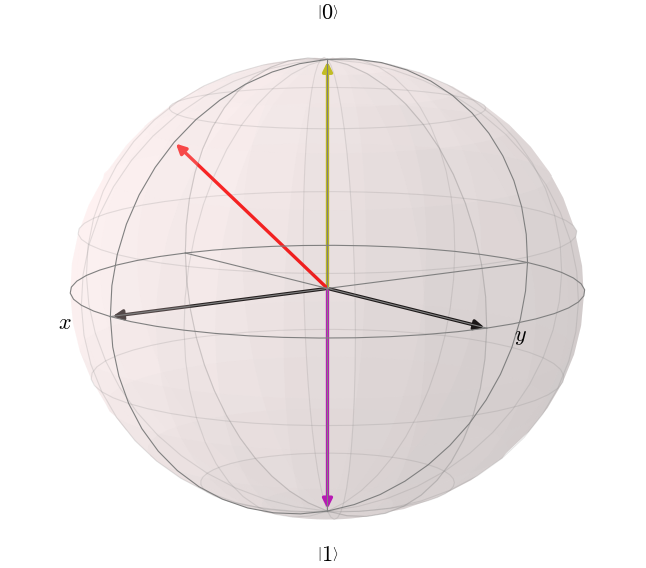
\includegraphics[scale=0.5]{img/3over4state.png}
       \caption{\label{fig:3over4}Simple binary classification problem of a quantum state}
\end{figure}

\begin{minipage}[c]{.49\textwidth}
    \begin{tabular}{| C{0.8cm} | C{1.7cm} |C{2cm}|}
      \toprule
      Qubit state & Vector representation & Class\\
      \midrule
       $\ket{0}$ & $\colvec{1\\0}$ & $\ket{0}$ (yellow)\\\midrule
       $\ket{1}$ & $\colvec{0\\1}$ & $\ket{1}$ (purple)\\\midrule
      \bottomrule
    \end{tabular}
        \label{tab:trainingset}
        \captionsetup{justification=raggedright, singlelinecheck=false}
    \captionof{table}{Training set}
\end{minipage}%%%%
\begin{minipage}[c][][b]{.49\textwidth}
\flushright
    \begin{tabular}{| C{2.7cm} | C{2.3cm} |C{2cm}|}
      \toprule
      Qubit state & Vector representation & Expected class\\
      \midrule
       $e^{-i\frac{\pi}{8}}\big[0.92388\ket{0} + 0.38268\ket{1}\big]$ & $e^{-i\frac{\pi}{8}}\colvec{0.92388\\0.38268}$ & $\ket{0}$ (yellow)\\\midrule
      \bottomrule
    \end{tabular}
        \label{tab:inputvectors}
        \captionsetup{justification=raggedleft, singlelinecheck=false}
    \captionof{table}{Input vector}
\end{minipage}

\subsubsection{Initial state preparation}
\label{subsubsubsec:initialstatepreparation}

The first step towards an actual implementation of this problem is to prepare the initial quantum state $\ket{\psi_0}$ previously defined in Equ.~\ref{equ:ampinitial} to be of the form,
\begin{equation}
\label{equ:ampinitial2}
\ket{\psi_0} = \frac{1}{\sqrt{2M}}\sum_{m=1}^{M} (\textcolor{emerald}{\ket{0}}\ket{\textcolor{red}{\Psi_{x}}}+\textcolor{emerald}{\ket{1}}\ket{\textcolor{darkyellow}{\Psi}_{\textcolor{purple}{t^{m}}}})\ket{c^{m}}\ket{m}
\end{equation}

where in the case of the selected classification problem:
\begin{align} 
\label{equ:vectordefs}
&\ket{\textcolor{red}{\Psi_{x}}} = e^{-i\frac{\pi}{8}}\big[0.92388\ket{0} + 0.38268\ket{1}\big]\\
&\ket{\textcolor{darkyellow}{\Psi_{t^{1}}}} = \ket{0} \\
&\ket{\textcolor{purple}{\Psi_{t^{2}}}} = \ket{1}
\end{align}
 
Since there are only two training vectors the index $m$ in Equ.~\ref{equ:ampinitial2} only takes the values 1 and 2. However, the $m$ qubit can only take binary values such that we need to redefine $1\rightarrow 0$ and $2\rightarrow 1$. With this observation, the required number of qubits can be deduced from Equ.~\ref{equ:ampinitial2}: one ancilla, one qubit for input and training vectors, one class qubit and one $m$ qubit making a total of four qubits. In the subsequent discussion the quantum state of the IBM QC in the $i^{th}$ step will be denoted $\ket{\chi_i}$. Since all qubits in the IBM Quantum Composer are initialized in state \0 the initial state $\ket{\chi_0}$ is simply,
\begin{equation}
\ket{\chi_0} = \ket{a}\ket{d}\ket{c}\ket{m} = \ket{0}\ket{0}\ket{0}\ket{0}
\end{equation}

where $a$ stands for ancilla, $d$ for data, $c$ for class and $m$ for the $m$ qubit. The sum over $m$ is introduced by simply acting an H gate on the $m$ qubit:
\begin{equation}
\ket{\chi_1} = (\mathbb{1} \otimes \mathbb{1} \otimes \mathbb{1} \otimes H)\ket{0}\ket{0}\ket{0}\ket{0} = \frac{1}{\sqrt{2}} \sum_{m=0}^1 \ket{0}\ket{0}\ket{0}\ket{m}
\end{equation}
%ADD CIRCUIT REPRESENTATION?

Using another H gate, the ancilla qubit is put in superposition:
\begin{equation}
\ket{\chi_2} = (H \otimes \mathbb{1} \otimes \mathbb{1} \otimes \mathbb{1})\ket{\chi_1} = \frac{1}{2} \sum_{m=0}^1 \ket{0}\ket{0}\ket{0}\ket{m} + \ket{1}\ket{0}\ket{0}\ket{m} = \frac{1}{2} \sum_{m=0}^1 \big[ \ket{0}\ket{0} + \ket{1}\ket{0}\big] \ket{0}\ket{m}
\end{equation}
%ADD CIRCUIT REPRESENTATION?

Next, the input vector $\ket{\textcolor{red}{\Psi_{x}}}$ should be loaded into the quantum state by means of a yet unknown gate sequence $GS$ such that the state is described by,

\begin{align}
\label{equ:chi3}
\ket{\chi_3} &= GS \ket{\chi_2} = \frac{1}{2} \sum_{m=0}^1 \big[ \ket{0}\ket{\textcolor{red}{\Psi_{x}}} + \ket{1}\ket{0}\big] \ket{0}\ket{m}\notag\\
&= \frac{1}{2} \sum_{m=0}^1 \Big[ \ket{0}\textcolor{red}{e^{-i\frac{\pi}{8}}\big[0.92388\ket{0} + 0.38268\ket{1}\big]} + \ket{1}\ket{0}\Big] \ket{0}\ket{m}
\end{align}

By looking closely at Fig.~\ref{fig:3over4} one can deduce that the red input vector can be reached by simply rotating the \0 vector by an angle of $\frac{\pi}{4}$ around the y-axis. A y-rotation by an arbitrary angle $\vartheta$ can be achieved with the rotation operator $R_y(\vartheta)$. As described by \citeA{nielsen2010quantum}, $R_y(\vartheta)$ can be represented as a unitary 2x2 matrix and is obtained from exponentiating the Y gate as shown in Equ.~\ref{equ:rydef}.

\begin{equation}
\label{equ:rydef}
R_y(\vartheta) = e^{-i\vartheta\frac{Y}{2}} = \text{cos}\frac{\vartheta}{2}\mathbb{1} - i\text{sin}\frac{\vartheta}{2}Y = \begin{pmatrix}
\text{cos}\frac{\vartheta}{2} & -\text{sin}\frac{\vartheta}{2} \\
\text{sin}\frac{\vartheta}{2} & \text{cos}\frac{\vartheta}{2}
\end{pmatrix}
\end{equation}

At this point, note that $R_y(\vartheta)$ is not an element of IBM's universal gate set. The problem of how to implement $R_y(\vartheta)$ on the IBM QC will be addressed later. For now, suppose $R_y(\frac{\pi}{4})$ can be implemented. Acting this gate on the data qubit in $\ket{\chi_2}$ yields the expression

\begin{equation}
(\mathbb{1} \otimes R_y(\frac{\pi}{4}) \otimes \mathbb{1} \otimes \mathbb{1})\ket{\chi_2} = \frac{1}{2} \sum_{m=0}^1 \big[ \ket{0}\ket{\textcolor{red}{\Psi_{x}}} + \ket{1}\ket{\textcolor{red}{\Psi_{x}}}\big] \ket{0}\ket{m}
\end{equation}

This, however, is not the desired state $\ket{\chi_3}$ defined in Equ.~\ref{equ:chi3} since the input vector $\ket{\textcolor{red}{\Psi_{x}}}$ should only be entangled with the \0 state of the ancilla. To achieve this type of entanglement the controlled version of the y-rotation gate, $CR_y(\frac{\pi}{4})(c,t)$, is required. When applying it using the $a$ qubit as control and the $d$ qubit as target the input vector will be entangled with the \1 state of the ancilla. Flipping the $a$ qubit with an X gate moves the input vector to the \0 state of the ancilla. Hence, the desired state $\ket{\chi_3}$ is obtained by applying the following gate sequence $GS$:
\begin{equation}
\label{equ:gs}
GS = (X \otimes \mathbb{1} \otimes \mathbb{1} \otimes \mathbb{1}) (CR_y(\frac{\pi}{4})(a,d) \otimes \mathbb{1} \otimes \mathbb{1}) \\
\end{equation}
subbing into Equ.~\ref{equ:chi3}:
\begin{align}
\label{equ:chi3prepared}
\ket{\chi_3} &=  GS \ket{\chi_2} = (X \otimes \mathbb{1} \otimes \mathbb{1} \otimes \mathbb{1}) (CR_y(\frac{\pi}{4})(a,d) \otimes \mathbb{1} \otimes \mathbb{1}) \ket{\chi_2}\notag\\
&= (X \otimes \mathbb{1} \otimes \mathbb{1} \otimes \mathbb{1}) \Big[\frac{1}{2} \sum_{m=0}^1 \big[\ket{0}\ket{0} + \ket{1}\ket{\textcolor{red}{\Psi_{x}}}\big] \ket{0}\ket{m}\Big]\notag\\
&= \frac{1}{2} \sum_{m=0}^1 \Big[ \ket{0}\ket{\textcolor{red}{\Psi_{x}}} + \ket{1}\ket{0}\Big] \ket{0}\ket{m}
\end{align}

It is important to note that also $CR_y(\frac{\pi}{4})(c,t)$ is not an element of IBM's universal gate set. Its implementation on the IBM QC will be discussed in the next subsection.

The next step is to entangle the first training vector $\ket{\textcolor{darkyellow}{\Psi_{t^{0}}}}$  with the \1 state of the ancilla and the \0 state of the $m$ qubit. Additionally, the second training vector $\ket{\textcolor{purple}{\Psi_{t^{1}}}}$ should be entangled with the \1 states of the ancilla and the $m$ qubit. Note that $\ket{\textcolor{darkyellow}{\Psi_{t^{1}}}}$ and $\ket{\textcolor{purple}{\Psi_{t^{2}}}}$ defined in Equ.~\ref{equ:vectordefs} were redefined to $\ket{\textcolor{darkyellow}{\Psi_{t^{0}}}}$ and $\ket{\textcolor{purple}{\Psi_{t^{1}}}}$ respectively. Expanding the sum in Equ.~\ref{equ:chi3prepared} demonstrates that $\ket{\textcolor{darkyellow}{\Psi_{t^{0}}}} = \ket{0}$ is already at its desired place:

\begin{align}
\label{equ:chi3expanded}
\ket{\chi_3} &= \frac{1}{2}\Big[ \big[\ket{0}\ket{\textcolor{red}{\Psi_{x}}} + \ket{1}\ket{0}\big] \ket{0}\ket{0} + \big[ \ket{0}\ket{\textcolor{red}{\Psi_{x}}} + \ket{1}\ket{0}\big] \ket{0}\ket{1}\Big]\notag\\
&= \frac{1}{2}\Big[ \big[\ket{0}\ket{\textcolor{red}{\Psi_{x}}} + \ket{1}\ket{\textcolor{darkyellow}{\Psi_{t^{0}}}}\big] \ket{0}\ket{0} + \big[ \ket{0}\ket{\textcolor{red}{\Psi_{x}}} + \ket{1}\ket{0}\big] \ket{0}\ket{1}\Big]
\end{align}

In order to entangle $\ket{\textcolor{purple}{\Psi_{t^{1}}}}$ with the \1 states of the ancilla and $m$ qubit a Toffoli (CCNOT) gate needs to be implemented. Using the ancilla ($a$) and $m$ qubit as controls and choosing the data ($d$) qubit as target one obtains the following state:

\begin{align}
\label{equ:chi4}
\ket{\chi_4} &= CCNOT(a,m,d)\ket{\chi_3}\notag\\
&= \frac{1}{2}\Big[ \big[\ket{0}\ket{\textcolor{red}{\Psi_{x}}} + \ket{1}\ket{\textcolor{darkyellow}{\Psi_{t^{0}}}}\big] \ket{0}\ket{0} + \big[ \ket{0}\ket{\textcolor{red}{\Psi_{x}}} + \ket{1}\ket{1}\big] \ket{0}\ket{1}\Big]\notag\\
&= \frac{1}{2}\Big[ \big[\ket{0}\ket{\textcolor{red}{\Psi_{x}}} + \ket{1}\ket{\textcolor{darkyellow}{\Psi_{t^{0}}}}\big] \ket{0}\ket{0} + \big[ \ket{0}\ket{\textcolor{red}{\Psi_{x}}} + \ket{1}\ket{\textcolor{purple}{\Psi_{t^{1}}}}\big] \ket{0}\ket{1}\Big]
\end{align}

The class qubit for the first training vector is already in the correct \0 state. Note again that also the CCNOT gate is not element of IBM's universal gate set which will be addressed later.

It remains to flip the class qubit for the second training vector by applying a CNOT gate using the $d$ qubit as control and the class($c$) qubit as target. The resulting state is then given by,

\begin{align}
\label{equ:chi5}
\ket{\chi_5} &= CNOT(d,c)\ket{\chi_4}\notag\\
&= \frac{1}{2}\Big[ \big[\ket{0}\ket{\textcolor{red}{\Psi_{x}}} + \ket{1}\ket{\textcolor{darkyellow}{\Psi_{t^{0}}}}\big] \ket{\textcolor{darkyellow}{0}}\ket{0} + \big[ \ket{0}\ket{\textcolor{red}{\Psi_{x}}} + \ket{1}\ket{\textcolor{purple}{\Psi_{t^{1}}}}\big] \ket{\textcolor{purple}{1}}\ket{1}\Big]
\end{align}

and can be rewritten as:

\begin{align}
\label{equ:chi5psi0}
\ket{\chi_5} &= \frac{1}{2} \sum_{m=1}^{2} \big[\ket{0}\ket{\textcolor{red}{\Psi_{x}}} + \ket{1}\ket{\textcolor{darkyellow}{\Psi_{t^{0}}}}\big] + \big[ \ket{0}\ket{\textcolor{red}{\Psi_{x}}} + \ket{1}\ket{\textcolor{purple}{\Psi_{t^{1}}}}\big]\ket{c^{m}}\ket{m}\notag\\
&= \frac{1}{2} \sum_{m=1}^{2} \big[\ket{0}\ket{\textcolor{red}{\Psi_{x}}} + \ket{1}\ket{\textcolor{darkyellow}{\Psi_{\textcolor{purple}{t^{m}}}}}\big]\ket{c^{m}}\ket{m}
\end{align}

When comparing Equ.~\ref{equ:chi5psi0} to $\ket{\psi_0}$ in Equ.~\ref{equ:ampinitial} it becomes clear that $\ket{\chi_5}$ is in the form of the desired initial quantum state $\ket{\psi_0}$. The quantum state preparation is therefore theoretically completed.

\subsubsection{Decomposition of a controlled-U gate}
\label{subsubsubsec:controlledugate}

To implement the quantum state preparation on the IBM QC, it remains to find a way of realizing the controlled y-rotation $CR_y(\frac{\pi}{4})(c,t)$ using only the ten gates from IBM's universal gate set. In their book \citeA{nielsen2010quantum} describe how a controlled U (CU) gate can be decomposed into a sequence of CNOT and single qubit gates. Thereby, U can be any unitary single-qubit gate. A CU gate is then defined as:
\begin{equation}
CU = \begin{pmatrix}
 \mathbb{1} & 0 \\ 
 0 & U
 \end{pmatrix}
\end{equation}

Most of the time the CU gate cannot be implemented directly since it is not element of the universal gate set at hand and it has to be realized through larger quantum circuits. Fig.~\ref{img:cudecomposition} shows the decomposition described by \citeA{nielsen2010quantum} into two CNOTs, three unitary single-qubit gates $A,B,C$ and a phase-adjusting matrix which will be denoted $P$ of the form:
\begin{equation}
P = \begin{pmatrix}
 1 & 0 \\ 
 0 & e^{i\alpha}
 \end{pmatrix}
\end{equation}

\begin{figure}[ht]
   \centering
   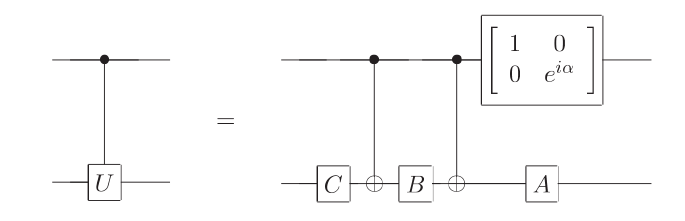
\includegraphics[width=0.7\textwidth]{img/controlledudecomp.png}
   \caption[]{Circuit decomposition of controlled-U quantum gate.\footnotemark[14]}
   \label{img:cudecomposition}
\end{figure}

\footnotetext[14]{Reprinted from Michael A. Nielsen and Isaac L. Chuang. Quantum Computation and Quantum Information. Cambridge University Press, 2000. Copyright 2010 by Nielsen \& Chuang.}

The idea of this decomposition is that when the control qubit (top qubit in Fig.~\ref{img:cudecomposition}) is \0 the gate combination $ABC$ is applied to the target qubit (bottom qubit in Fig.~\ref{img:cudecomposition}) and has to equal the identity gate:

\begin{equation}
\label{equ:abcidentity}
ABC = \mathbb{1}
\end{equation}

If and only if the control qubit is \1 then the gate sequence $e^{i\alpha}AXBXC$ is applied to the target. Since the goal is to apply the unitary U to the target qubit the following equation must be satified:
\begin{equation}
\label{equ:UAXBXC}
e^{i\alpha}AXBXC = U
\end{equation}

\citeA{nielsen2010quantum} make the following choices for the unitary gates $A,B,C$:

\begin{align}\label{equ:abc}
A &=  R_z(\beta)R_y(\frac{\gamma}{2})\\
B &= R_y(-\frac{\gamma}{2})R_z(-\frac{\delta+\beta}{2})\\
C &= R_z(\frac{\delta-\beta}{2})
\end{align}

where $R_z(\varrho)$ is the general rotation gate about the z-axis of the Bloch sphere. Similary to the $R_y(\vartheta)$ gate it can be obtained by exponentiating the Z gate as shown below in Equ.~\ref{equ:rzdef}.

\begin{equation}
\label{equ:rzdef}
R_z(\varrho) = e^{-i\varrho\frac{Z}{2}} = \text{cos}\frac{\varrho}{2} \mathbb{1}- i\text{sin}\frac{\varrho}{2}Z = \begin{pmatrix}
e^{-i\frac{\varrho}{2}} & 0 \\
0 & e^{i\frac{\varrho}{2}}
\end{pmatrix}
\end{equation}

When subbing the expressions for $A,B,C$ from Equ.~\ref{equ:abc} into Equ.~\ref{equ:abcidentity} one will indeed obtain the identity operation (proof omitted). These choices of $A,B,C$ are also a solution to Equ.~\ref{equ:UAXBXC}. Subbing into Equ.~\ref{equ:UAXBXC} leads to the following expression for matrix $U$:

\begin{equation}
\label{equ:udecompdef}
U = \begin{pmatrix}
 e^{i(\alpha-\frac{\beta}{2}-\frac{\delta}{2})}\cos{\frac{\gamma}{2}} & -e^{i(\alpha-\frac{\beta}{2}+\frac{\delta}{2})}\sin{\frac{\gamma}{2}} \\ 
e^{i(\alpha+\frac{\beta}{2}-\frac{\delta}{2})}\sin{\frac{\gamma}{2}} & e^{i(\alpha+\frac{\beta}{2}+\frac{\delta}{2})}\cos{\frac{\gamma}{2}}
 \end{pmatrix}
\end{equation}
%Furthermore, \citeA{nielsen2010quantum} show that any unitary matrix U can be decomposed as,
%\begin{equation}
%\label{equ:URzRyRz}
%U = e^{i\alpha}R_z(\beta)R_y(\gamma)R_z(\delta)
%\end{equation}
%\begin{equation}
%\label{equ:UAXBXC}
%e^{i\alpha}AR_x(\pi)BR_x(\pi)C = U
%\end{equation}

To decompose $CR_y(\frac{\pi}{4})$, one simply chooses $U = R_y(\frac{\pi}{4})$. Subbing $\vartheta = \frac{\pi}{4}$ into Equ.~\ref{equ:rydef} the matrix representation of $R_y(\frac{\pi}{4})$ is obtained:

\begin{equation}
U = R_y(\frac{\pi}{4}) = \begin{pmatrix}
\text{cos}\frac{\pi}{8} & -\text{sin}\frac{\pi}{8} \\
\text{sin}\frac{\pi}{8} & \text{cos}\frac{\pi}{8}
\end{pmatrix}
\end{equation}

Subbing this expression for $U$ into Equ.~\ref{equ:udecompdef} leads to:

\begin{equation}
\label{equ:udecompsubbed}
U = \begin{pmatrix}
\text{cos}\frac{\pi}{8} & -\text{sin}\frac{\pi}{8} \\
\text{sin}\frac{\pi}{8} & \text{cos}\frac{\pi}{8}
\end{pmatrix} = \begin{pmatrix}
 e^{i(\alpha-\frac{\beta}{2}-\frac{\delta}{2})}\cos{\frac{\gamma}{2}} & -e^{i(\alpha-\frac{\beta}{2}+\frac{\delta}{2})}\sin{\frac{\gamma}{2}} \\ 
e^{i(\alpha+\frac{\beta}{2}-\frac{\delta}{2})}\sin{\frac{\gamma}{2}} & e^{i(\alpha+\frac{\beta}{2}+\frac{\delta}{2})}\cos{\frac{\gamma}{2}}
 \end{pmatrix}
\end{equation}

When setting the expressions for the respective matrix entries in Equ.~\ref{equ:udecompsubbed} equal, the following system of non-linear complex equations is obtained :

\begin{align}
\label{equ:nlsystem}
\text{cos}\frac{\pi}{8} &= e^{i(\alpha-\frac{\beta}{2}-\frac{\delta}{2})}\cos{\frac{\gamma}{2}}\\
-\text{sin}\frac{\pi}{8} &= -e^{i(\alpha-\frac{\beta}{2}+\frac{\delta}{2})}\sin{\frac{\gamma}{2}}  \\
\text{sin}\frac{\pi}{8} &= e^{i(\alpha+\frac{\beta}{2}-\frac{\delta}{2})}\sin{\frac{\gamma}{2}}\\
\text{cos}\frac{\pi}{8} &= e^{i(\alpha+\frac{\beta}{2}+\frac{\delta}{2})}\cos{\frac{\gamma}{2}}\\
\end{align}

This is a system of four non-linear complex equations with four unknowns. In order to solve for the parameters $\alpha,\beta,\gamma$ and $\delta$ one can use any root finding algorithm for non-linear equations such as Secant or Newton's method. Using Newton's method the solutions are found to be:
\begin{equation}
\alpha =  \pi; \quad 
\beta = 2\pi;\quad 
\delta = \frac{7}{8}\pi;\quad 
\gamma = 0
\end{equation}

Subbing these parameters into the expressions for $A,B$ and $C$ defined in Equ.~\ref{equ:abc} yields,

\begin{align}
\label{equ:abcsubbed1}
A \quad= \quad R_z(\beta)R_y(\frac{\gamma}{2})\quad =& \quad R_z(2\pi) \quad = \quad \textcolor{emerald}{\mathbb{1}} \\
\label{equ:abcsubbed2}
B\quad =\quad R_y(-\frac{\gamma}{2})R_z(-\frac{\delta+\beta}{2})\quad =& \quad R_z(-\frac{23}{16}\pi) \quad= \quad \textcolor{red}{?}  \\
\label{equ:abcsubbed3}
C \quad=\quad R_z(\frac{\delta-\beta}{2})\quad =& \quad R_z(-\frac{9}{16}\pi) \quad= \quad \textcolor{red}{?} \\
\label{equ:abcsubbed4}
P\quad =\quad \begin{pmatrix} 1&0\cr0&e^{i\alpha} \end{pmatrix}\quad=& \quad \begin{pmatrix} 1&0\cr0&e^{i\pi} \end{pmatrix}\quad= \quad \textcolor{emerald}{Z}
\end{align}

Quantum gate $A$ is just equal to the identity gate which certainly is element of IBM's universal gate set. The phase-adjusting gate $P$ is equal to the Z gate that also is within IBM's gate set. Only gates $B$ and $C$ result in more complex z-rotations of $-\frac{23}{16}\pi$ and $-\frac{9}{16}\pi$ radians respectively. Unfortunately, these quantum gates are not found in IBM's gate set as indicated by the red question marks in Equ.~\ref{equ:abcsubbed2} and \ref{equ:abcsubbed3}.

\subsubsection{The Solovay-Kitaev theorem}
\label{subsubsubsec:solovaykitaev}

An important theorem in quantum information is the Solovay-Kitaev theorem first proposed by Robert M. Solovay and later published by \citeA{kitaev1995quantum}. It will be used to decompose the quantum gates $B$ and $C$ into a sequence of quantum gates from IBM's universal gate set.

At this point, it is important to remember that any universal quantum gate set is a dense subset of the special unitary group $SU(2)$ as previously defined in Section~\ref{subsubsec:qubits}.

\begin{redbox}
\textbf{Theorem: Solovay-Kitaev theorem}\\
\newline
Let $G$ be a universal quantum set $G$ consisting of quantum gates from $SU(2)$ and let $\epsilon > 0$ be a desired accuracy. Then there is a constant $b$ such that for any single-qubit gate $W \in SU(2)$ there exists a
finite gate sequence $\tilde{G}$ of gates from the set $G$ of length $O(log^b (1/\epsilon))$ such that $d(W, \tilde{G}) < \epsilon$. In their proof, \citeA{dawson2005solovay} show that $b \approx 3.97$.\\
\newline
In other words, given a set of single-qubit quantum gates which is a dense subset of $SU(2)$, then the Solovay-Kitaev theorem guarantees that this set will quickly fill $SU(2)$.
\cite{dawson2005solovay}.
\end{redbox}

The Solovay-Kitaev theorem is important because it proofs that given any universal gate set it is possible to obtain good approximations to any desired single-qubit gate $W$. In their paper, \citeA{dawson2005solovay} describe how to design an algorithm implementing the Solovay-Kitaev theorem. Unfortunately, the Solovay-Kitaev algorithm needs to be implemented on a classical computer which adds to the overall time complexity of the quantum compiling process as will be shown later. For this thesis, the open-source software package 'Quantum Compiler, v0.03'\footnotemark[15] developed in Python by Paul Pham was used to run the Solovay-Kitaev algorithm described by \citeA{dawson2005solovay}. This software package compares different gate approximations to the desired gate by a new distance metric called Fowler distance.

\footnotetext[15]{The software package 'Quantum Compiler, v0.03' by Paul Pham can be downloaded from \url{https://sourceforge.net/projects/quantumcompiler/files/v0.03/}.}

\begin{redbox}
\textbf{Definition: Fowler distance}\\
\newline
When approximating a unitary gate $W$ with a gate sequence yielding another unitary gate $W_{approx}$ it is important to quantify how 'close' the action of $W_{approx}$ is to $W$. The Fowler distance makes use of the matrix representations of $W$ and $W_{approx}$ and is defined by \citeA{booth2012quantum} as:
\begin{equation}
d(W,W_{approx}) = \sqrt{\frac{2-\mid tr(W\cdot W_{approx}^\dagger)\mid}{2}}
\end{equation}

In contrast to $W$, $W_{approx}$ might introduce a shift in the global phase of the quantum state it is acting on. However, since the global phase of a quantum state is immeasurable in experiment it can be neglected. As a result, the Fowler distance is defined in such a way that possible global phase differences are ignored.
\end{redbox}

Subsequently, the desired gates $B = R_z(-\frac{23}{16}\pi)$ and $C = R_z(-\frac{9}{16}\pi)$ where decomposed using the Solovay-Kitaev algorithm. Fig.~\ref{fig:skresultplot} shows a plot visualizing how the Fowler distance depends on the number of gates in the approximating gate sequence $W_{approx}$. The number of gates in the approximating gate sequence is also called \emph{gate count}. The plot clearly shows an exponential increase in the gate count for decreasing Fowler distance. For example, 146 gates suffice to achieve $d(W_{approx},R_z(-\frac{9}{16}\pi)) = 0.04389$. Yet, already 17,838 gates are required to reduce the Fowler distance to $d(W_{approx},R_z(-\frac{9}{16}\pi)) = 0.01008$.

\begin{figure}[H]
\centering
    \begin{tikzpicture}[scale=1]
\begin{axis}[xlabel={Gate count},ylabel={Fowler distance [$d(U,U_{approx})$]}]

% Graph column 2 versus column 0
\addplot table[x index=1,y index=0,col sep=comma] {datax.dat};
\addlegendentry{$R_z(-\frac{9}{16}\pi)$}% y index+1 since humans count from 1

% Graph column 1 versus column 0    
\addplot table[x index=5,y index=4,col sep=comma] {datax.dat};
\addlegendentry{$R_z(-\frac{23}{16}\pi)$}

\end{axis}
\end{tikzpicture}
\caption{Fowler distance plotted against the required gate count for quantum gates $B = R_z(-\frac{23}{16}\pi)$ and $C = R_z(-\frac{9}{16}\pi)$ }
\label{fig:skresultplot}
  \end{figure}
  
Fowler distance is best understood with a visual example using the gate $B = R_z(-\frac{23}{16}\pi)$. Acting the desired gate $B$ on the state $\ket{\psi} = \frac{\ket{0} + \ket{1}}{\sqrt{2}}$ (black vector in Fig.~\ref{fig:bloch23over16}) results in the purple Bloch vector $\vec{b}$ shown in Fig.~\ref{fig:bloch23over16}.

\begin{figure}[H]
\centering
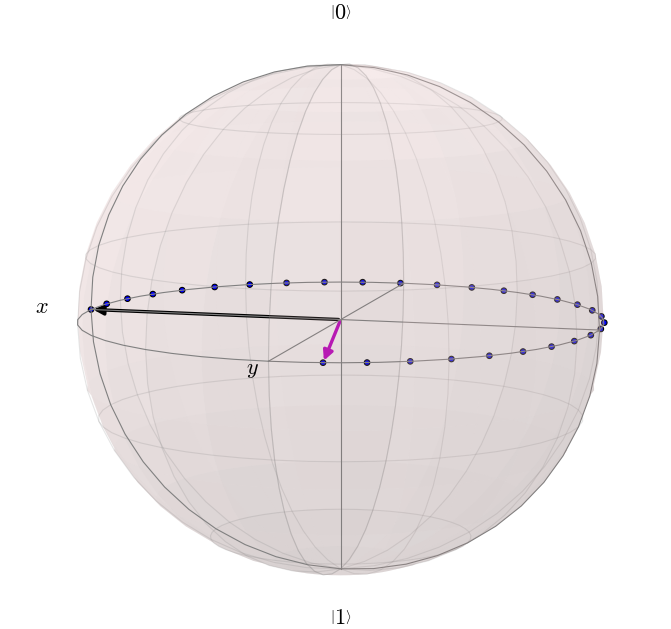
\includegraphics[scale=0.4]{img/bloch23over16.png}
\caption{\label{fig:bloch23over16} Action of $B = R_z(-\frac{23}{16}\pi)$ on the state $\ket{\psi} = \frac{\ket{0} + \ket{1}}{\sqrt{2}}$}
\end{figure}

Fig.~\ref{fig:fowlerdistances} shows the action of four different approximating gate sequences $B_{approx,1}$, $B_{approx,2}$, $B_{approx,3}$, $B_{approx,4}$ on the state $\ket{\psi} = \frac{\ket{0} + \ket{1}}{\sqrt{2}}$. Gate sequence $B_{approx,1}$ consists of 25 gates and is a Fowler distance of $d = 0.15165$ away from $B$. The resulting state vector is coloured green in Fig.~\ref{fig:fowlerdistances}. The green vector lies above the Bloch equator and is relatively far away from the desired vector $\vec{b}$ in Fig.~\ref{fig:bloch23over16}. With 109 gates, $B_{approx,2}$ yields a Fowler distance of $d = 0.10722$ resulting in the blue vector. It is also found below the Bloch equator and still relatively far from $\vec{b}$. Using $B_{approx,3}$ the Fowler distance drops to $d = 0.02086$ leading to the yellow vector in  Fig.~\ref{fig:fowlerdistances}. This vector is almost on the Bloch equator and relatively close to $\vec{b}$ implying that $B_{approx,3}$ is a good approximation of $B$. However, $B_{approx,3}$ already requires the implementation of 2,997 single-qubit gates. The purple vector from Fig.~\ref{fig:bloch23over16} is also plotted in Fig.~\ref{fig:fowlerdistances} but is not visible since the red vector with $d = 0.00158$ constitutes a very good approximation to the desired state $\vec{b}$.  The red vector is the result of the action of $B_{approx,4}$ which, unfortunately, needs 370,813 gates to achieve such a small Fowler distance. Hereby, Gate $B$ was used as an example but such an exponential increase in the gate count is observed for any quantum gate $W$ when applying the Solovay-Kitaev algorithm \cite{dawson2005solovay}.

\begin{minipage}[c]{.8\textwidth}
	%\vspace{-20mm}
	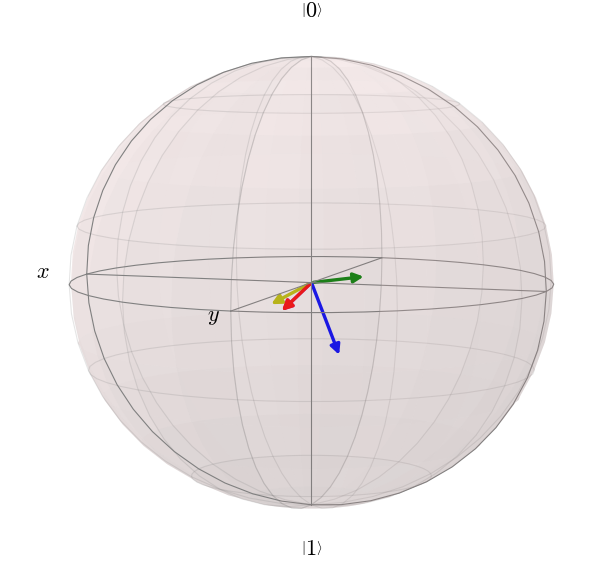
\includegraphics[height=0.8\textwidth]{img/fowlerdistances.png}
       \captionsetup{justification=raggedright, singlelinecheck=false}
       \captionof{figure}{\label{fig:fowlerdistances}Various Fowler distances visualized on Bloch sphere }
\end{minipage}%%%%%
\begin{minipage}[c]{.2\textwidth}
\begin{equation}
\textcolor{emerald}{d = 0.15165} \notag
\end{equation}
\begin{equation}
\textcolor{blue}{d = 0.10722} \notag
\end{equation}
\begin{equation}
\textcolor{darkyellow}{d = 0.02086} \notag
\end{equation}
\begin{equation}
\textcolor{red}{d = 0.00158} \notag
\end{equation}

\end{minipage}

Implementing any quantum gate $D$ inevitably takes some time $t$ since it involves the use of hardware components e.g. targeting a specific electron with a laser pulse. Based on IBM's single-qubit and CNOT gate times described in Section~\ref{subsec:ibmqc} the total execution time of twelve different gate sequences, approximating $B = R_z(-\frac{23}{16}\pi)$ and $C = R_z(-\frac{9}{16}\pi)$ to different Fowler distances, were calculated. The results can be seen in Table~\ref{tab:sktimes}. Keeping in mind that in the best case, the maximum decoherence time of a qubit in IBM's QC is \SI{112.4}{\micro\second} most gate sequences are too long for an IBM implementation (coloured red in Table~\ref{tab:sktimes}). Feasible execution times are marked green in Table~\ref{tab:sktimes}. However, decoherence is not the only limiting factor since IBM only allows for 39 gates and one measurement gate. But even when selecting the smallest sequences of 25 gates for $B$ and 16 gates for $C$, the total gate count is 41 which is two gates more than the allowed gate count of the IBM Quantum Composer. Furthermore, the approximating gate sequences of $B$ and $C$ are not the only gates needed to prepare the initial quantum state and execute the akNN algorithm. Unfortunately, this makes an actual implementation of this particular classification problem on IBM's QC impossible.

%Thus, the only possibility would be to select the sequence of 25 gates for $B$ and the sequence of 16 gates for $C$ at the cost of relatively large Fowler distances. This, however, still sums up to 41 gates which is two gates more than the allowed gate count of the IBM Quantum Composer. 

\begin{table}[H]
\centering
    \begin{tabular}{c| c |c |c }
      \toprule
      Approx. Gate & Fowler distance & Gate count & Execution time\\
      \midrule
      $R_z(-\frac{23}{16}\pi)$ & 0.15165 & 25 & \textcolor{emerald}{$\sim$\SI{3}{\micro\second}}\\
       & 0.10722 & 109 & \textcolor{emerald}{$\sim$\SI{14}{\micro\second}}\\
       & 0.02086 & 2,997 & \textcolor{red}{$\sim$\SI{390}{\micro\second}}\\
       & 0.01494 & 14,721 & \textcolor{red}{$\sim$\SI{1914}{\micro\second}}\\
       & 0.003327 & 74,009 & \textcolor{red}{$\sim$\SI{9621}{\micro\second}}\\
       & 0.001578 & 370,813 & \textcolor{red}{$\sim$\SI{48206}{\micro\second}}\\
       \midrule
      $R_z(-\frac{9}{16}\pi)$ & 0.28390 & 16 & \textcolor{emerald}{$\sim$\SI{2}{\micro\second}}\\
       & 0.04389 & 146 & \textcolor{emerald}{$\sim$\SI{18}{\micro\second}}\\
       & 0.049511 & 728 & \textcolor{emerald}{$\sim$\SI{87}{\micro\second}}\\
       & 0.02823 & 3,622 & \textcolor{red}{$\sim$\SI{435}{\micro\second}}\\
       & 0.01008 & 17,838 & \textcolor{red}{$\sim$\SI{2141}{\micro\second}}\\
       & 0.00156 & 444,646 & \textcolor{red}{$\sim$\SI{53358}{\micro\second}}\\
      \bottomrule
      \bottomrule
    \end{tabular}
    \caption{\label{tab:sktimes} Results of the Solovay-Kitaev algorithm for decomposition of $B = R_z(-\frac{23}{16}\pi)$ and $C = R_z(-\frac{9}{16}\pi)$}
  \end{table}
  
To complete the quantum compiling, assume that gates $B$ and $C$ could somehow be implemented with shorter gate sequences. It remains to decompose the Toffoli gate that was required to 'load' the second training pattern $\ket{\textcolor{purple}{\Psi_{t^{1}}}}$ into the quantum state $\ket{\chi_4}$ as shown in Equ.~\ref{equ:chi4}.

\subsubsection{Toffoli Gate Decomposition}
\label{subsubsubsec:toffoli}

The Toffoli or CCNOT gate can be decomposed into CNOT and single-qubit gates in several ways. In their book,\citeA{nielsen2010quantum} describe the decomposition into six CNOTs and nine single-qubit gates; two H gates, three T and three T$^\dagger$ gates. See Fig.~\ref{img:toffolidecomp} for the corresponding circuit diagram. This decomposition does not require any further compiling work since all involved gates are elements of IBM's universal gate set.

\begin{figure}[!ht]
       \centering
       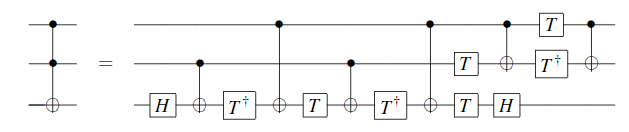
\includegraphics[scale=0.5]{img/toffolidecomposition.png}
       \caption[]{\label{img:toffolidecomp} Decomposition of a Toffoli gate into six CNOT and nine single-qubit gates\footnotemark[16]}
\end{figure}

\footnotetext[16]{Reprinted from Michael A. Nielsen and Isaac L. Chuang. Quantum Computation and Quantum Information. Cambridge University Press, 2000. Copyright 2010 by Nielsen \& Chuang.}

The Toffoli decomposition finalizes the compiling of the quantum state preparation into gates from IBM's gate set only. In summary, the compiled state preparation requires: 2 H gates applied to the ancilla and the $m$ qubit, the decomposed $CR_y(\frac{\pi}{4})$ gate (2 CNOTs, 1 Z gate, 1 $\mathbb{1}$ gate (can be neglected) \& a sequence of minimum 25 gates for $B$ and minimum 16 gates for $C$), 1 X gate to flip the ancilla (Equ.~\ref{equ:chi3prepared}), 1 decomposed Toffoli (6 CNOTs, 2 H gates, 3 T \& 3 T$^\dagger$ gates) to load the second training vector and 1 CNOT to flip the class qubit. Thus, the quantum state preparation was compiled into 9 CNOT and 53 single-qubit gates. The akNN algorithm only requires one additional H gate and two measurement gates (for ancilla and class qubit) leading to a total of 9 CNOT, 54 single-qubit gates and 2 measurement gates. However, even cleverly arranging these gates does not suffice to implement the algorithm within IBM's 40 gate slots. The full circuit diagram for the compiled state preparation and the akNN algorithm can be seen in Fig.~\ref{img:toffolidecomp}.

\begin{figure}[!ht]
       \centering
       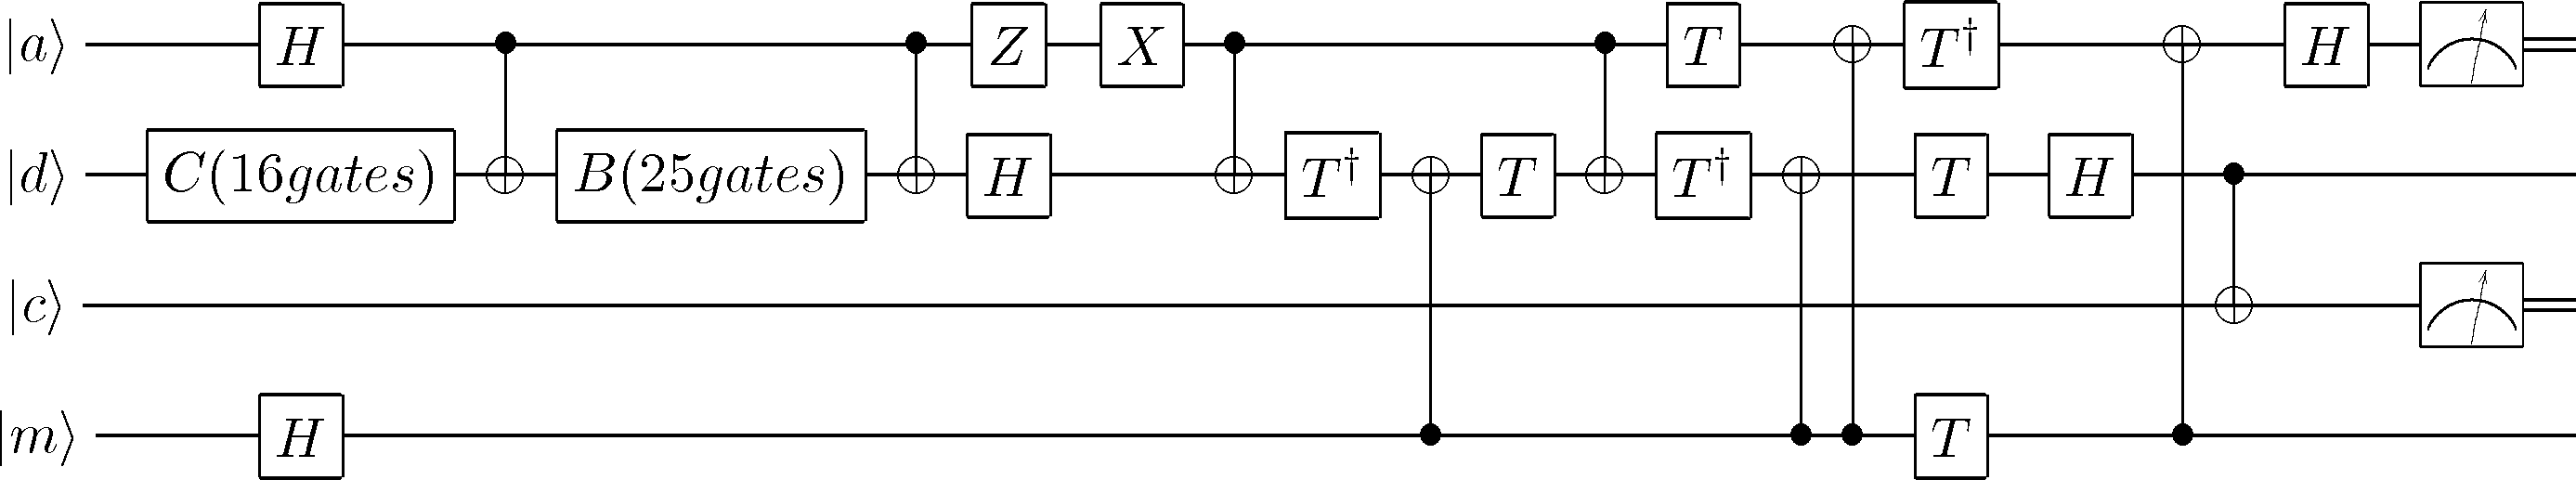
\includegraphics[width=\textwidth]{img/fullQKNN.png}
       \caption[]{\label{img:toffolidecomp} Compiled quantum circuit for implementing the akNN algorithm with the binary Bloch vector classification problem}
\end{figure}

%state preparation
%H Gate m qubit
%H Gate ancilla
%CR_y decomposed
%X Gate ancilla
%Toffoli(a,m,d)
%CNOT(d,c)

%algorithm
%H ancilla
%CM ancilla
%M class

%Final circuit diagram showing the compile state preparation + akNN algorithm steps

\begin{greenbox}
\textbf{Complexity analysis including quantum compiling steps}\\
\newline
The akNN algorithm itself was found to run in constant time $\mathcal{O}(\frac{1}{Prob(CM)})$. However, to determine the overall algorithmic complexity all steps required to prepare the initial quantum state $\ket{\psi_0}$ from Equ.~\ref{equ:ampinitial} need to be included. The decomposition of the $CR_y(\frac{\pi}{4})$ gate involved solving a system of non-linear equations by means of a root-finding algorithm. Any iterative root-finding algorithm e.g. Secant or Newton's method has a complexity of $\mathcal{O}(k)$ where $k$ is the number of root finding iterations. Furthermore, the Solovay-Kitaev algorithm was required to find two single-qubit gate sequences approximating the two gates $B = R_z(-\frac{23}{16}\pi)$ and $C = R_z(-\frac{9}{16}\pi)$. According to \citeA{dawson2005solovay} the Solovay-Kitaev algorithm has a complexity of $\mathcal{O}(m*log^{2.71}(\frac{m}{\epsilon}))$ for $\epsilon$-approximations of $m$ gates. Thus the total complexity is given by:
\begin{equation}
\mathcal{O}(\frac{1}{Prob(CM)})+\mathcal{O}(k)+\mathcal{O}(m*log^{2.71}(\frac{m}{\epsilon}))
\end{equation}
	
When adding algorithmic complexities only the most dominant term is considered relevant. Thus, the overall complexity including state preparation is found to be $\mathcal{O}(m*log^{2.71}(\frac{m}{\epsilon}))$.\\
\newline
In conclusion, due to the necessary quantum compiling steps the initial constant complexity of the akNN algorithm
\begin{equation}  
\mathcal{O}(\frac{1}{Prob(CM)})
\end{equation}
increased to a polylogarithmic complexity of
\begin{equation}
\mathcal{O}(m*log^{2.71}(\frac{m}{\epsilon}))
\end{equation}
dependening on the number of gates $m$ that need $\epsilon$-approximations by means of the Solovay-Kitaev algorithm.
\end{greenbox}

%All in all, it was shown that for this particular classification problem the constant complexity of the aKNN algorithm is dominated by the complexity of the quantum compiling. 

\subsection{Simulating the amplitude-based kNN algorithm}
\label{subsubsec:simulationamplitudeKNN}

Since the IBM Quantum Experience does not allow for an implementation, the aKNN algorithm was simulated in Liqui$\ket{}$ to determine the performance and the outcome of the algorithm. This section is subdivided into two parts: First, the classification of Bloch vectors described in the last section is simulated. Second, the aKNN algorithm is used to classify different Gaussian distributions constituting a slightly more complex classification task.

\subsubsection{Classification of Bloch vectors}
\label{subsubsubsec:classificationblochvectors}

The Bloch vector classification problem described in Section~\ref{subsubsec:implementationamplitudeKNN} was reconsidered and simulated in Liqui$\ket{}$ to determine if the algorithm yields the expected classification outcome. 

Section~\ref{subsubsec:implementationamplitudeKNN} pointed out that the implementation of the controlled y-rotation $CR_y(\frac{\pi}{4})$ was the main issue preventing an implementation within IBM's 40 gate slots. However, by specifying its matrix representation Liqui$\ket{}$ allows any unitary single- or multi-qubit gate to be defined within its programming framework. Therefore, $CR_y(\frac{\pi}{4})$ can be easily implemented in Liqui$\ket{}$. This enables to load the input vector specified in Table~\ref{tab:inputvectors} without having to decompose the controlled y-rotation gate and with no need for the Solovay-Kitaev algorithm. Due to this enormous simplification of the quantum state preparation routine, a second input vector was considered for simulation. Fig.~\ref{img:7over8} shows the new second input vector on the Bloch sphere. This new input vector can be obtained by rotating the \0 state by $\frac{\pi}{8}$ radians around the y-axis. The resulting new input data set is listed in Table~\ref{tab:inputvectors2}.

Table~\ref{tab:inputvectors2} shows that the probability of measuring the new input vector (ID=2) in state \0 is slightly higher than for the input vector with ID=1. This can also be seen visually when comparing Fig.~\ref{img:7over8} to Fig.~\ref{fig:3over4}. Lastly, the training data set listed in Table~\ref{tab:trainingset} was not altered for simulation.

\begin{table}[H]
\centering
\begin{tabular}{| C{0.5cm} | C{2.7cm} | C{2.3cm} |C{2cm}|}
      \toprule
      ID & Qubit state & Vector representation & Expected class\\
      \midrule
       1 & $e^{-i\frac{\pi}{8}}\big[0.92388\ket{0} + 0.38268\ket{1}\big]$ & $e^{-i\frac{\pi}{8}}\colvec{0.92388\\0.38268}$ & $\ket{0}$ (yellow)\\\midrule
       2 & $e^{-i\frac{\pi}{16}}\big[0.98079\ket{0} + 0.19509\ket{1}\big]$ & $e^{-i\frac{\pi}{16}}\colvec{0.98079\\0.19509}$ & $\ket{0}$ (yellow)\\\midrule
      \bottomrule
    \end{tabular}
    \caption{\label{tab:inputvectors2} Input data set II for the simulation of the aKNN algorithm. The data set consists of two different qubit states both lying in the z-x plane of the Bloch sphere.}
\end{table}

\begin{figure}[H]
       \centering
       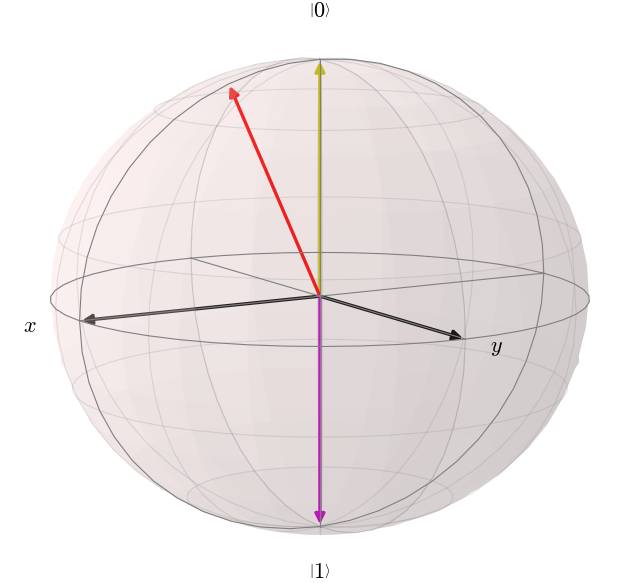
\includegraphics[scale=0.5]{img/bloch7over8.png}
       \caption{\label{img:7over8} Visualization of the second input qubit state $e^{-i\frac{\pi}{16}}\big[0.98079\ket{0} + 0.19509\ket{1}\big]$ coloured red on the Bloch sphere. The first training vector \0 is shown in yellow and the second training vector \1 is shown in purple.}
\end{figure}

The obtained simulation results after 1000 runs for both Bloch vectors from input data set II are shown in Table~\ref{tab:blochresults}. The theoretically predicted probabilities are marked with asterisks and are always displayed on top of the corresponding simulation result. Comparing these values shows strong agreement between prediction and simulation implying that 1000 simulation runs suffice to retrieve the expected probability distributions.

\begin{table}[H]
\begin{tabular}{| C{0.5cm} | C{2.7cm} |C{1.7cm} | C{1.7cm} | C{1.7cm} |C{1.8cm}| C{1.8cm}|}
      %\toprule
      ID & Qubit state  & $Prob(CM)$ & $Prob$ $(\ket{c} = \ket{0})$ & $Prob$ $(\ket{c} = \ket{1})$ & Expected class & Algorithm output\\
      \midrule
        1 & $e^{-i\frac{\pi}{8}}\big[0.92388\ket{0} + 0.38268\ket{1}\big]$ & \begin{tabular}{c} 0.8266* \\\midrule 0.8050 \end{tabular} & \begin{tabular}{c} 0.5818* \\\midrule 0.5863 \end{tabular} & \begin{tabular}{c} 0.4182* \\\midrule 0.4137 \end{tabular} & $\ket{0}$ (yellow) & $\ket{0}$ (yellow)\\\midrule
        
       2 & $e^{-i\frac{\pi}{16}}\big[0.98079\ket{0} + 0.19509\ket{1}\big]$ & \begin{tabular}{c} 0.7940* \\\midrule 0.7710 \end{tabular} & \begin{tabular}{c} 0.6237* \\\midrule 0.6420 \end{tabular} & \begin{tabular}{c} 0.3763* \\\midrule 0.3580 \end{tabular} & $\ket{0}$ (yellow) & $\ket{0}$ (yellow)\\\midrule
      \bottomrule
    \end{tabular}
    \caption{\label{tab:blochresults} Classification results for two qubit states after 1000 runs. Input state with ID=1 was defined in Table~\ref{tab:inputvectors} and qubit state with ID=2 was defined in Section~\ref{subsubsec:simulationamplitudeKNN}. Trained with training set defined in Table~\ref{tab:trainingset} consisting of the \0 and \1 qubit states. Theoretical predictions (marked with asterisks) on top, simulation results at the bottom.}
\end{table}

Both input qubit states were correctly classified as \0 (yellow vector in Fig.~\ref{img:3over4} and Fig.~\ref{fig:7over8}) as expected since both qubit states lie within the upper half of the Bloch sphere. The input qubit state with ID=2 has a slightly higher probability of being classified as \0 than the qubit state with ID=1. This is expected since the state with ID=2 is closer to the training state \0 on the Bloch sphere than the state with ID=1. 	

In conclusion, using the small input data set II the amplitude-based kNN algorithm has achieved 100\% accuracy. However, since only two Bloch vectors were considered this number should not be taken too seriously but rather be seen as a small test bench for the amplitude-based kNN algorithm. All in all, the main purpose of this simulation was to show that the amplitude-based kNN algorithm would have performed as expected when an implementation with IBM's quantum computer would have been feasible.

The classification of Bloch vectors considered in this section only made use of one qubit for each training and input vector. Since one qubit can only be in a superposition of maximally two states (e.g. the \0 and \1 state) only two amplitudes, e.g. one for the \0 and one for the \1 state, are available for data encoding. This was deliberately chosen since it made it relatively easy to construct the initial quantum state (Equ.~\ref{equ:ampinitial}) required for the amplitude-based kNN algorithm. The next section will increase the number of qubits used to encode each training and input vector and will describe how the simulated amplitude-based kNN algorithm can be used to classify different Gaussian distributions.

\subsubsection{Classification of Gaussian distributions}
\label{subsubsubsec:classificationblochvectors}

Section~\ref{subsubsec:classicaldataamplitudes} introduced the idea of encoding classical data into the $2^n$ amplitudes of a quantum state with $n$ qubits leading to exponential data compression compared to classical computers. Initializing arbitrary amplitude distributions is still actively researched and as discussed in Section~\ref{subsubsec:classicaldataamplitudes} requires the use of non-trivial quantum algorithms. However, this section will demonstrate and use the fact that it is relatively easy to initialize Gaussian amplitude distributions.

Consider the following classical probability vector $w$ with eight entries representing a discrete Gaussian distribution:

\begin{equation}
w = \colvec{0.58566\\0.11434\\0.11434\\0.022322\\0.11434\\0.022322\\0.022322\\0.0043579}
\end{equation}

The goal is to initialize an amplitude distribution of a multi-qubit system such that it represents the classical vector $w$. Since $w$ has eight entries the multi-qubit system needs to consist of three qubits giving rise to $2^3=8$ amplitudes. Thus, the desired quantum memory state $\ket{w}$ representing the classical vector $w$ should be of the form:

\begin{align}
\label{equ:desiredmemorystate}
\ket{w} = \quad &0.58566 \ket{000} + 0.11434 \ket{001} + 0.11434 \ket{010} +
0.02232 \ket{011}\notag\\
&+ 0.11434 \ket{100} + 0.02232 \ket{101} + + 0.02232 \ket{110} 
+ 0.00436 \ket{111}
\end{align}

Knowing that the classical vector $w$ is Gaussian-distributed it follows that the amplitudes of $\ket{w}$ are also Gaussian-distributed which will become important later. To initialize the state $\ket{w}$ a suitable quantum gate is required. For this purpose, the idea of a coin operator can be borrowed from the theory of quantum random walks (CITATION). Such a coin operator can be used as a quantum gate to initialize a Gaussian distribution centered around a chosen binary qubit pattern as will be shown later. For this purpose, the coin gate, denoted $C$, will be defined as the following unitary matrix:

\begin{equation}
C(\delta) = \begin{pmatrix}
\sqrt{\delta} & 1-\sqrt{\delta} \\
1-\sqrt{\delta} & -\sqrt{\delta}
\end{pmatrix}
\end{equation}

where $0 \leq \delta \leq 1$. The action of $C(\delta)$ on a quantum state needs to be analyzed to understand how it can be used to create Gaussian-distributed quantum states and how the parameter $\delta$ influences the shape of these distributions. For example, acting $C(\delta)$ on each individual qubit in the three-qubit state $\ket{000}$ yields:

\begin{align}
&(C(\delta) \otimes C(\delta) \otimes C(\delta)) \ket{000} = C(\delta)\ket{0} \otimes C(\delta)\ket{0} \otimes C(\delta)\ket{0}\notag\\
&\equiv \begin{pmatrix}
\sqrt{\delta} & 1-\sqrt{\delta} \\
1-\sqrt{\delta} & -\sqrt{\delta}
\end{pmatrix} \colvec{1\\0} \otimes \begin{pmatrix}
\sqrt{\delta} & 1-\sqrt{\delta} \\
1-\sqrt{\delta} & -\sqrt{\delta}
\end{pmatrix} \colvec{1\\0} \otimes \begin{pmatrix}
\sqrt{\delta} & 1-\sqrt{\delta} \\
1-\sqrt{\delta} & -\sqrt{\delta}
\end{pmatrix} \colvec{1\\0}\notag\\
&= \colvec{\sqrt{\delta}\\1-\sqrt{\delta}} \otimes \colvec{\sqrt{\delta}\\1-\sqrt{\delta}} \otimes \colvec{\sqrt{\delta}\\1-\sqrt{\delta}}\notag\\
&= \colvec{\sqrt{\delta}*\colvec{\sqrt{\delta}\\1-\sqrt{\delta}}\\(1-\sqrt{\delta})*\colvec{\sqrt{\delta}\\1-\sqrt{\delta}}} \otimes \colvec{\sqrt{\delta}\\1-\sqrt{\delta}}\notag\\
&= \colvec{\delta\\\sqrt{\delta}-\delta\\\sqrt{\delta}-\delta\\1-2\sqrt{\delta}+\delta} \otimes \colvec{\sqrt{\delta}\\1-\sqrt{\delta}}\notag\\
\label{equ:deltatensor}
&= \colvec{\delta\sqrt{\delta}\\\delta-\delta\sqrt{\delta}\\\delta-\delta\sqrt{\delta}\\\sqrt{\delta}(\delta+1)-2\delta\\\delta-\delta\sqrt{\delta}\\\sqrt{\delta}(\delta+1)-2\delta\\\sqrt{\delta}(\delta+1)-2\delta\\-\sqrt{\delta}(3+\delta)+1+3\delta}
\end{align}

When choosing $\delta = 0.7$, the last expression in Equ.~\ref{equ:deltatensor} is equal to the desired quantum memory state $\ket{w}$ defined in Equ.~\ref{equ:desiredmemorystate}:

\begin{align}
\label{equ:deltatensorsubbed}
\ket{w} &= \colvec{0.58566\\0.11434\\0.11434\\0.022322\\0.11434\\0.022322\\0.022322\\0.0043579}\notag\\
&\equiv 0.58566 \ket{000} + 0.11434 \ket{001} + 0.11434 \ket{010} +
0.02232 \ket{011}\notag\\
&\quad \quad + 0.11434 \ket{100} + 0.02232 \ket{101} + + 0.02232 \ket{110} 
+ 0.00436 \ket{111}
\end{align}

Thus, it was shown that acting $C(0.7)$ on each qubit in the state $\ket{000}$ yields the desired quantum memory state $\ket{w}$. Since the amplitudes of $\ket{w}$ represent a discretized Gaussian distribution, it was shown that the coin gate $C(\delta)$ can indeed be used to generate Gaussian amplitude distributions. 

Keeping in mind that $\ket{w}$ resulted from the action of $(C(0.7) \otimes C(0.7) \otimes C(0.7))$ onto the $\ket{000}$ state and important pattern is observed when calculating the Hamming distances between $\ket{000}$ and all eight possible three qubit states. Firstly, the state $\ket{000}$ has a Hamming distance of zero relative to itself and has the highest amplitude of 0.58566. Secondly, $\ket{100}$, $\ket{010}$ and $\ket{001}$ all have amplitudes of 0.11434 and a Hamming distance of one with respect to $\ket{000}$. Thirdly, $\ket{110}$, $\ket{011}$ and $\ket{101}$ have amplitudes of 0.02232 and a Hamming distance of two compared to $\ket{000}$. Lastly, $\ket{111}$ has a Hamming distance of three with respect to $\ket{000}$ and an amplitude of 0.00436. Hence, the amplitudes are always equal for equal Hamming distances and decrease with increasing Hamming distance.

To visualise the Gaussian distribution represented by $\ket{w}$, one simply needs to plot amplitudes against Hamming distances and mirror the resulting plot with respect to the vertical line connecting the horizontal zero value with the data point representing the highest amplitude. The corresponding plot is given in Fig.~\ref{fig:gaussdeltaplot1} and clearly shows a discrete Gaussian distribution centered around the binary qubit pattern with Hamming distance zero: in this case $\ket{000}$. It follows that applying the coin gate $C(0.7)$ to each qubit in an $n$-qubit systems $\ket{q_1,q_2,...,q_n}$ yields a similar discretized Gaussian distribution centered around the binary qubit pattern $\ket{q_1,q_2,...,q_n}$.
%redefine the Hamming distance between $\ket{100}$ and $\ket{000}$ to be -1 instead of 1 and the Hamming distance between $ket{110}$ and $\ket{000}$ to be -2 instead of 2. Furthermore, suppose one can add a ninth entry to $\ket{w}$ by duplicating the entry for state $\ket{111}$. Define the new duplicate entry of $\ket{111}$ to have a Hamming distance of -3 instead of 3. When plotting the Hamming distances against the amplitudes of this new artificial vector representation of $\ket{w}$ a discrete Gaussian distribution can be observed. The corresponding plot in Fig.~\ref{fig:gaussdeltaplot1} illustrates this clearly.

\begin{figure}[H]
\centering
    \begin{tikzpicture}[scale=1]
\begin{axis}[xlabel={Hamming distance},ylabel={Amplitude},
				xtick=data,xticklabel style={align=center},xticklabels={3,2,1,0,1,2,3}]
				
				%xticklabels={{3\\($\ket{111}$)},{2\\($\ket{011}$)\\($\ket{110}$)\\($\ket{101}$)},{1\\($\ket{100}$)\\($\ket{010}$)\\($\ket{001}$)},{0\\($\ket{000}$)},{1\\($\ket{100}$)\\($\ket{010}$)\\($\ket{001}$)},{2\\($\ket{011}$)\\($\ket{110}$)\\($\ket{101}$)},{3\\($\ket{111}$)}}]

% Graph column 0 versus column 1
\addplot table[x index=1,y index=0,col sep=comma] {gauss2.dat};
\addlegendentry{$\delta = 0.7$}% y index+1 since humans count from 1

\end{axis}
\end{tikzpicture}
\caption{Plot visualizing the discrete Gaussian distribution of $\ket{w}$ resulting from acting coin gate $C$ with $\delta =0.7$ on each qubit in state $\ket{000}$. Amplitudes of quantum state $\ket{w}$ (Equ.~\ref{equ:desiredmemorystate}) are plotted against the Hamming distances between binary pattern $\ket{000}$ and all eight binary three-qubit pattern. The plot was mirrored with respect to the vertical line connecting the horizontal zero value with the data point representing the highest amplitude.}
\label{fig:gaussdeltaplot1}
  \end{figure}
  
The observed pattern within the amplitudes can be generalized using Equ.~\ref{equ:deltatensor}: Acting the coin gate $C(\delta)$ on each qubit in the three-qubit state $\ket{000}$ will result in a discretized Gaussian distribution centered around $\ket{000}$ with the following amplitudes dependent on the Hamming distance with respect to state $\ket{000}$: state $\ket{000}$ with Hamming distance zero will have the largest amplitude of $\delta\sqrt{\delta}$, states with Hamming distance one have amplitudes equal to $\delta-\delta\sqrt{\delta}$, states with Hamming distance two have amplitudes equal to $\sqrt{\delta}(\delta+1)-2\delta$ and the state $\ket{111}$ with the largest Hamming distance of three has the smallest amplitude of $-\sqrt{\delta}(3+\delta)+1+3\delta$.
  
A useful tool for visualizing Hamming distances between three-qubit patterns is a three-dimensional cube as shown in Fig.~\ref{img:cubenoprobs}. On that cube, adjacent qubit patterns have a Hamming distance (HD) of one and the Hamming distance increases by one with every additional corner. For example, the qubit state $\ket{100}$ is adjacent to $\ket{110}$ since they only differ in one qubit ($HD=1$). Moving one more corner yields the state $\ket{111}$ or $\ket{010}$ which both have a Hamming distance of two when compared to $\ket{100}$.

\begin{figure}[!ht]
       \centering
       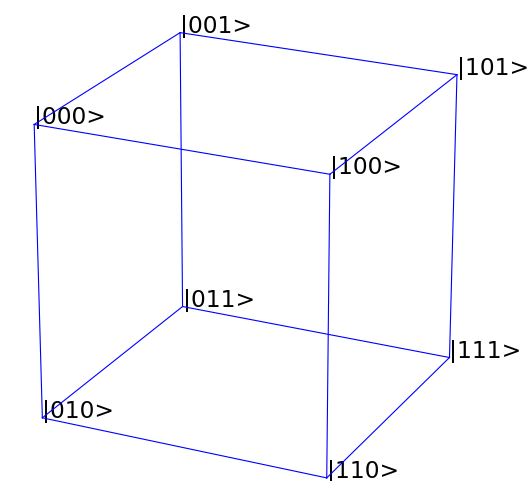
\includegraphics[width=0.5\textwidth]{img/cubewithoutprobs.png}
       \caption{\label{img:cubenoprobs} Visualizing Hamming distances on a three-dimensional cube. The Hamming distance between two binary qubit patterns is given by the shortest path on the edges of the cube between them. Thereby, the Hamming distance increases by one for every corner.}
\end{figure}

This cube can be used as another way of visualizing the action of the coin gate $C(0.7)$ on each qubit in the e.g. $\ket{000}$ state. Before applying the $C$ gates the qubit state is $\ket{000}$ with an amplitude of 1.0 shown in Fig.~\ref{img:cubeoneprob} wherein amplitude is denoted by $a$.
  
\begin{figure}[H]
       \centering
       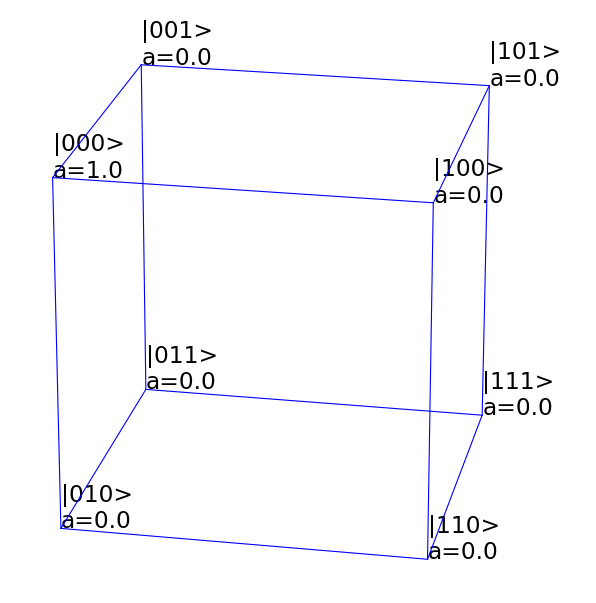
\includegraphics[width=0.5\textwidth]{img/cubeoneprob.png}
       \caption{\label{img:cubeoneprob} The qubit state $\ket{000}$ with amplitude ($a$) of 1.0 visualized on a three-dimensional cube representing the Hamming distances between binary qubit patterns.}
\end{figure}

Applying the coin gate $C$ to the first qubit redistributes the amplitudes between the $\ket{000}$ and $\ket{100}$ state which is visualized in Fig.~\ref{img:cubediffused1} below.

\begin{figure}[H]
       \centering
       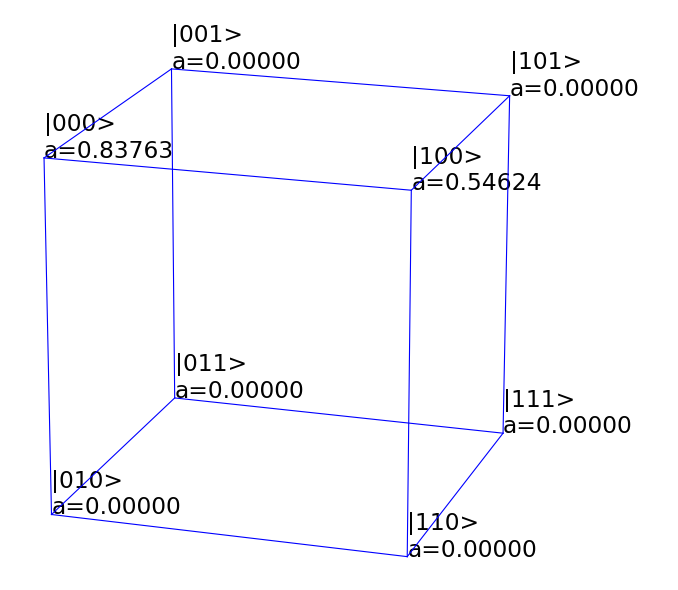
\includegraphics[width=0.5\textwidth]{img/cube_diffused1.png}
       \caption{\label{img:cubediffused1} Visualization of the amplitude distribution over all three-qubit states after application of coin gate $C$ to the first qubit of the state $\ket{000}$.}
\end{figure}

Fig.~\ref{img:cubediffused2} illustrates the amplitude distribution after application of $C$ gates to the first and second qubit in the state $\ket{000}$. It can be seen that only four out of eight three-qubit states have non-zero amplitudes at this point. With the application of the third $C$ gate to the third qubit in $\ket{000}$ all eight qubit patterns have non-zero amplitudes and the quantum state $\ket{w}$ from Equ.~\ref{equ:desiredmemorystate} is obtained. Fig.~\ref{img:cubediffused3} shows this final quantum superposition representing a discrete Gaussian distribution over a three-dimensional cube based on Hamming distances.

In this example, Fig.~\ref{img:cubediffused1}, ~\ref{img:cubediffused2} and \ref{img:cubediffused3} visually demonstrate a stepwise diffusion of the initial amplitude of 1.0 from $\ket{000}$ over all eight three-qubit patterns on the cube.

\begin{minipage}[c]{.5\textwidth}
       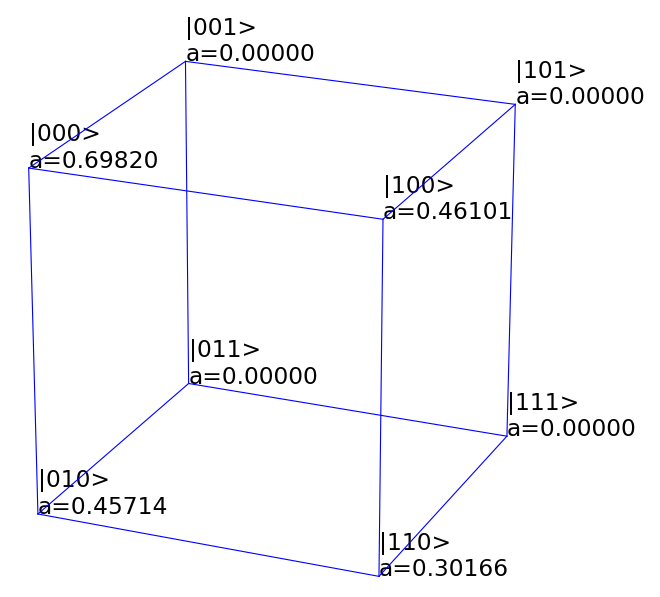
\includegraphics[width=1\textwidth]{img/cube_diffused2.png}
       \captionsetup{justification=raggedright, singlelinecheck=false}
       \captionof{figure}{\label{img:cubediffused2} Visualization of the amplitude distribution over all three-qubit states after application of coin gate $C$ to the first two \\qubits in the state $\ket{000}$.}
\end{minipage}%%%%%
\begin{minipage}[c]{.5\textwidth}
       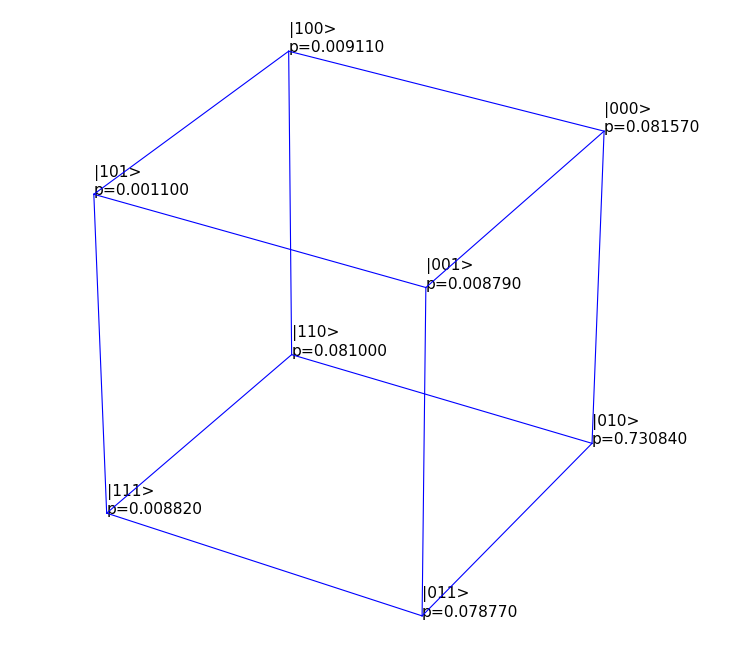
\includegraphics[width=1\textwidth]{img/cube_diffused.png} \captionsetup{justification=raggedright, singlelinecheck=false}
       \captionof{figure}{\label{img:cubediffused3} Final amplitude distribution over all three-qubit states after application of coin gate $C$ to each qubit in the state $\ket{000}$ visualized on a three-dimensional cube.}
\end{minipage}


\begin{figure}[H]
\centering
    \begin{tikzpicture}[scale=1.3]
\begin{axis}[xlabel={Hamming distance},ylabel={Probability},xtick=data,xticklabels={4,3,2,1,0,1,2,3,4}]

% Graph column 0 versus column 1
\addplot table[x index=1,y index=0,col sep=comma] {gauss1.dat};
\addlegendentry{$\delta = 0.9$}% y index+1 since humans count from 1

% Graph column 2 versus column 1 
\addplot table[x index=1,y index=2,col sep=comma] {gauss1.dat};
\addlegendentry{$\delta = 0.8$}

% Graph column 3 versus column 1    
\addplot table[x index=1,y index=3,col sep=comma] {gauss1.dat};
\addlegendentry{$\delta = 0.7$}

% Graph column 4 versus column 1    
\addplot table[x index=1,y index=4,col sep=comma] {gauss1.dat};
\addlegendentry{$\delta = 0.6$}

% Graph column 5 versus column 1   
\addplot table[x index=1,y index=5,col sep=comma] {gauss1.dat};
\addlegendentry{$\delta = 0.5$}

\end{axis}
\end{tikzpicture}
\caption{Gaussian distributions}
\label{fig:gaussdeltaplot2}
  \end{figure}

This way of visualizing HDs can be extended to the 16 binary patterns made by four qubits that can be visualized on a 4-D cube, also called tesseract, as illustrated in Fig.~\ref{img:hypercubenoprobs}.

\begin{figure}[!ht]
       \centering
       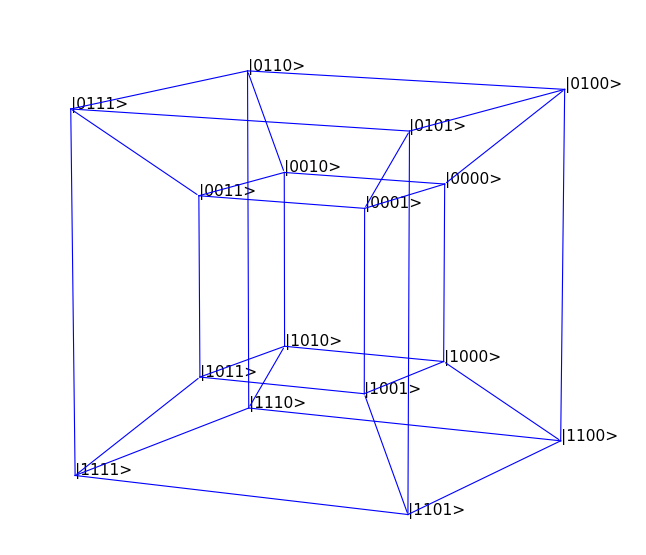
\includegraphics[width=0.5\textwidth]{img/hypercubewithoutprobs.png}
       \caption{\label{img:hypercubenoprobs} Visualizing Hamming distances on a 4-D cube (tesseract)}
\end{figure}


Initializing gaussian distributed quantum states and classifying gaussian distributions by means of the Hellinger distance.

\begin{redbox}
\textbf{Definition: Hellinger distance}\\
\newline
The Hellinger distance is a distance metric used to quantify the difference between any two probability distributions. In the case of continuous probability distributions it is defined using the Hellinger integral first proposed by \citeA{hellinger1909neue}. However, since the $2^n$ amplitudes of an $n$-qubit system will always constitute a discrete probability distribution only the Hellinger distance for discrete distributions will be introduced.\\
\newline
According to \citeA{harsha}, the Hellinger distance between two probability distributions $R = (r_1,...,r_j)$ and $T = (t_1,...,t_j)$ is defined as:

\begin{equation}
\label{equ:hellingerdistance}
H(R,T) = \frac{1}{\sqrt{2}}\sqrt{\sum_{i=1}^j (\sqrt{r_i} - \sqrt{t_i})^2}
\end{equation}

and can be rewritten in terms of the Euclidean distance between the square root vectors $\sqrt{R}$ and $\sqrt{T}$:

\begin{equation}
H(R,T) = \frac{1}{\sqrt{2}} \mid\mid\sqrt{R} - \sqrt{T}\mid\mid_2
\end{equation}
\end{redbox}

\begin{equation}
Prob(\ket{c^m} = \ket{1(\textcolor{purple}{B})})= \sum_{m \mid c^m=1(\textcolor{purple}{B})} 1 - \frac{1}{4M} \sum_{i=1}^N \mid \textcolor{red}{x_i} - \textcolor{purple}{t^m_i} \mid ^2
\end{equation}

Hence, if $x_i = \sqrt{w_i}$ where $w_i$ is the i\textsuperscript{th} element of the classical probability vector $w$ the aKNN algorithm classification outcome is dependent on the squared Hellinger distance. This can be obtained by squaring Equ.~\ref{equ:hellingerdistance} yielding:
\begin{equation}
\label{equ:squaredhellingerdistance}
H^2(R,T) = \frac{1}{\sqrt{2}}\sum_{i=1}^j (\sqrt{r_i} - \sqrt{t_i})^2
\end{equation}







